\documentclass[conference]{IEEEtran}

% correct bad hyphenation here
\hyphenation{op-tical net-works semi-conduc-tor}
\usepackage{graphicx}
\usepackage[square, numbers, comma, sort&compress]{natbib}
\usepackage{verbatim} 
\usepackage{vector}
\usepackage{amsthm}
\usepackage{array}
\usepackage{tabularx}
\usepackage{multirow}
\usepackage{fixltx2e}
\usepackage[english]{babel}
\usepackage{amsmath}
\usepackage{todonotes}
\usepackage[]{algorithm2e}
\usepackage{pgfplots}
\usepackage{caption}
\usepackage{url}
\usepackage{pdfpages}

\begin{document}
\title{An Efficient Approach for Mining Frequent Pattern over Uncertain Data Stream}

\author{
    \IEEEauthorblockN{Md. Badi-Uz-Zaman Shajib\IEEEauthorrefmark{1}, Md. Samiullah\IEEEauthorrefmark{1}, Chowdhury Farhan Ahmed\IEEEauthorrefmark{2}, Carson Kai-Sang Leung\IEEEauthorrefmark{3}}
    \IEEEauthorblockA{\IEEEauthorrefmark{1}Department of Computer Science \& Engineering, University of Dhaka, Bangladesh
    \\mbzshajib@gmail.com, samiullah@cse.univdhaka.edu}
    \IEEEauthorblockA{\IEEEauthorrefmark{2}ICube Laboratory, University of Strasbourg, France
    \\cfahmed@unistra.fr}
    \IEEEauthorblockA{\IEEEauthorrefmark{3}Department of Computer Science University of Manitoba, Canada
    \\kleung@cs.manitoba.ca}
}

% make the title area
\maketitle

\begin{abstract}
Knowledge discovery in big data is one of the most recent, interesting and popular topic in state-of-the-art research where frequent patterns finding is one of the important challenges. With the rapid growth of modern technology huge amount of data is flowing all over the world. Moreover, the incoming stream of data is not always accurate and precise. Properties of data stream flow changing each and every time with the change of interest of people that is making data dynamic.  These uncertain stream data (e.g. GPS data, satellite monitoring, biometric data etc.) are the resources to many emerging applications in various real life applications like medical sciences, disaster management and national security. Many approaches have been developed to find frequent patterns from uncertain data. Some works emphasized on finding frequent patterns from the stream of uncertain data. Due to the uncertainty and dynamic properties of data, it becomes a great challenge to find the appropriate and efficient approach to ensure the efficient usage of available resources. In the adopted approaches there is a tradeoff between optimization (probabilistic approach and allowing false data in final result) and correctness (exact calculation and minimum resource usage). Moreover, most of them cannot handle the stream of data, that is, dynamic databases. In this paper, we have proposed a probabilistic sliding window based efficient and optimized approach for handling uncertain data stream. We have proposed a new memory efficient and optimized data structure, i.e., US-tree (Uncertain Stream-tree) that stores most recent meta-information for mining. A comprehensive performance analysis shows that our approach is scalable, correct and efficient in comparison with the recent related approaches.
\end{abstract}

% no keywords




% For peer review papers, you can put extra information on the cover
% page as needed:
% \ifCLASSOPTIONpeerreview
% \begin{center} \bfseries EDICS Category: 3-BBND \end{center}
% \fi
%
% For peerreview papers, this IEEEtran command inserts a page break and
% creates the second title. It will be ignored for other modes.
\IEEEpeerreviewmaketitle


\section{Introduction}

Knowledge Discovery in Databases (KDD) is one of the most recent and interesting fields of research. Knowledge discovery in databases (KDD) has been created to identify efficient, helpful and valuable information from extreme large databases. The main goal of this field is to find the frequent, interesting and functional information from extremely large databases and use extract valuable information in different applications and research work. Discovered Knowledge can then be used to provide automated analysis and solutions to business. It has attracted a significant amount of research.

In this KDD process, the result of data mining process is to find interesting, significant and useful patterns from massive data. In recent years, with increasing of modern technologies and huge use of internet there a lot of data is being produced. Extraction of important and significant patterns from this extreme large data repository and data sources is not that much easy. Moreover. relating these interesting patterns in real-life scenario is also very tough. The mining of useful and important information refers to the acquisition of previously unknown knowledge (e.g. frequent item-set) from extremely large data collections.

Data mining is defined as a process of discovering important, potentially useful and valuable patterns from extremely large volumes of data. In finding interesting and significant relations, support is used as an indicator to find out if the pattern is interesting or not. The term Data Mining or Knowledge Discovery in Databases have been adopted for a field of research dealing with the automatic discovery of implicit information or knowledge within databases. Data mining is generally utilized by organizations (e.g., financial, retail, marketing and communication organizations) with a strong consumer focus. Found knowledge from mining result of can be used to relating association rules between objects, incidents, processes, finding the actual and correct strategy to C2C (consumer to consumer) marketing, B2B (business to business) marketing, B2C (business to consumer) marketing, and other marketing policy determination etc. In telecommunication industry, finding interesting valuable patterns for multidimensional analysis of telecommunication data, fraudulent pattern analysis, unusual patterns identification, and mobile telecommunication services the pattern mining helps a lot. In the medical science, semantic integration of heterogeneous, distributed genomic and proteomic databases, alignment, indexing, similarity search and comparative analysis, multiple nucleotide sequences, pattern mining in KDD process is very helpful. Moreover, in data warehouses, for data pre-processing and different data visualization this data mining process is very useful. In genetic algorithm analysis and finding characteristic of human, frequent pattern mining process is used. Discovery of structural patterns, analysis of genetic networks and protein pathways, association and path analysis, visualization tools in genetic data analysis, data mining is very much effectively used process.

Data uncertainty is an inherent property in various applications due to reasons such as hardware fault, the uncertainty of incidents, outdated sources or imprecise/incorrect measurement. In the age of big data, uncertainty is one of the defining characteristics of data. Data is constantly growing in volume, variety, velocity and uncertainty. In a large range of applications domains uncertain data is found in abundance. Today on the World Wide Web, data from sensor networks like GPS, weather detection machines, within enterprises both in their structured and unstructured sources, biological data, meteorological trends, of the medical behavior of living organisms’ data, human behavior, are the example of uncertain data. Customer name of a super shop is a real life example of uncertain data. For example, there exist several customers named Mrs./Mr X registered in a super shop but if we want a particular Mrs./Mr. X then we will not certainly be able to find her/him by name.

In the modern age, there are much more instruments we are being used to like smart-phones, smart-gears (e.g. smart watch, smart glass). All the devices have many more sensors those are collecting data each and every micro second. But all the data from the sources are imprecise or incorrect. For example, a temperature sensor gives some information like current temperature is 40 degree, with 5\%-10\% error. This makes this data imprecise and uncertain. Moreover, features like weather forecast are inherently uncertain. For example, today's weather forecast may be rainy but it has only 65\% confidence. There are many cases when information acquired from human experiences is not reliable and precise. Different people can describe the same incident in different view and perspective. As an example, in a bird viewing event Mr. C saw a crow flying by. But, Mr. D thinks it was a raven. So, uncertainty values can be attached with these observations like the bird has 75\% probability to be crowd and 20\% probability to be a raven.
Tom mine interesting patterns from static database ~\cite{apriori}, ~\cite{fp_growth}, ~\cite{close_1}, ~\cite{closet}, ~\cite{closet_plus}, ~\cite{close_2} have been proposed. To solve finding interesting patterns from uncertain data several approaches has been proposed ~\cite{u_priori},, ~\cite{uf_growth}, ~\cite{ufp_growth}, ~\cite{uh_mining}, ~\cite{puf_growth}, ~\cite{cuf_growth}, ~\cite{uncertain_01}, ~\cite{uncertain_02}, ~\cite{uncertain_03}, ~\cite{uncertain_04}, ~\cite{uncertain_05}, ~\cite{uncertain_06}. For stream data mining ~\cite{ds_tree}, ~\cite{stream_01}, ~\cite{stream_02}, ~\cite{stream_03}, ~\cite{stream_04}, ~\cite{stream_05} has been proposed. But none of them can handle uncertain stream data. For uncertain stream data SUF-growth [~\cite{suf_growth} ] has been proposed. This is an exact algorithm. Constructed tree with this approach is very much sparse which affects in the mining process. 

Our key contributions of this paper are listed below:
\begin{itemize}
  \item We have introduced a prefix value, \emph{U\textsuperscript{cap}} for each item in a transaction which always maintains upper bound of probability. That helps us to make compact pattern tree construction.
  \item A new data-structure \emph{US-tree}, that is very much compact and very memory efficient.
  \item Propose a data-structure will follow the partial downward closure property.
  \item A new mining algorithm \emph{USFP-growth} algorithm, that will reduce mining time surprisingly.
  \item Propose an approach, which will both runtime and memory efficient, scalable and will have wide range of applicable area.
  \end{itemize}
We have carried out the thesis work to consummate the objectives. An outline of rest of the chapters is provided as follows. Chapter 2 describes the necessary related works and existing approaches. Chapter 3 provides the details of our proposed approach with required analysis. Experimental results in detail with comparison and analysis are given in Chapter 4. Chapter 5 ends the thesis with a brief conclusion and future scopes.

\section{Related Work}
%\documentclass{article} 
%\usepackage{graphicx}  
%\usepackage{multirow}
%\usepackage[table]{xcolor}
%\usepackage{fixltx2e}
%\usepackage{array}
%
%\begin{document}
\begin{table}
\centering

\begin{tabular}{|c|c|c|c|c|c|}
\hline
	Transaction No & \multicolumn{4}{c|}{Items in Transaction} \\ \hline \hline
	T\textsubscript{1} & a(0.9) & c(0.6) & d(0.5) & e(0.2)			\\\hline
	T\textsubscript{2} & a(0.9) & b(0.4) & e(0.1) & --    			\\\hline
	T\textsubscript{3} & a(0.2) & c(0.9) & d(0.7) & --    			\\\hline
	T\textsubscript{4} & b(0.3) & c(0.9) & -- & --			\\\hline
	T\textsubscript{5} & a(0.1) & b(0.3) & c(0.9) & --    			\\\hline
	T\textsubscript{6} & a(0.9) & e(0.3) & -- & --        			\\\hline
   	T\textsubscript{7} & a(0.1) & d(0.6) & e(0.2) & --		\\\hline
	T\textsubscript{8} & a(0.1) & c(0.2) & f(0.6) & --    			\\\hline
	T\textsubscript{9} & c(0.2) & d(0.9) & f(0.6) & --    			\\\hline
	
	T\textsubscript{10} &  --  &  --  &  --  & --    				\\\hline
	T\textsubscript{11} &  --  &  --  &  --  & --    				\\\hline
	T\textsubscript{12} &  --  &  --  &  --  & --    				\\\hline
			
\end{tabular}
\label{tab:ex_u}
\caption{Example of Uncertain Stream Transaction}
\label{table:uncertain_stream_transaction}
\end{table}
%\end{document}
Many algorithms have been developed for finding frequent item-sets from uncertain databases. Among them, some are Apriori ~\cite{apriori} like approach and others are FP-growth ~\cite{fp_growth} like approach. U-Apriori ~\cite{u_priori} was proposed to mine uncertain frequent pattern that is Apriori-like candidate generation and test-based approach. UF-growth ~\cite{uf_growth}, UFP-growth ~\cite{ufp_growth} was proposed to mine frequent patterns from uncertain data but the generated tree is not compact. CUF-growth ~\cite{cuf_growth}, CUF-growth\textsuperscript{*} ~\cite{cuf_growth}, PUF-growth ~\cite{puf_growth} was proposed later for mining uncertain data but they produce false positives as they works with probabilistic uncertainty modeling. All of them are unable to mine stream of uncertain data. UF-stream ~\cite{suf_growth} and SUF-growth ~\cite{suf_growth} proposed to mine uncertain frequent pattern from stream. UF-stream ~\cite{suf_growth} suffers from both false positives and false negatives. The SUF-growth ~\cite{suf_growth} is an exact mining algorithm that has resolved the false positive and false negative generation but the constructed tree structure is like UF-growth ~\cite{uf_growth} that suffers much because the data structure (tree) SUF-growth ~\cite{suf_growth} use to keep information is not compact. Before elaborate discussion of SUF-growth ~\cite{suf_growth} we will provide a brief discussion on the background of uncertain stream mining approaches.

UF-streaming ~\cite{suf_growth} was proposed to mine frequent item from uncertain stream data. This is a sliding window approach, that capture most recent data, as most recent data is most important. It has divided the transaction stream data in several batch each batch is inserted into the tree structure that is UF-tree ~\cite{uf_growth} and mine each tree using UF-growth ~\cite{uf_growth} and put all the frequent patterns found in a UF-stream structure. For avoiding false negative they have used a value \emph{preMinSup} less than minimum support (0 < \emph{preMinSup}< minimum support). Then until the window is completed the frequent item-set is put into UF-stream tree structure. This has addressed the problems of stream uncertain data mining, but it suffers from some problems like : Un-necessary mining each batch. Let window size is 3 and batch size is 2. If one wants the mining result at window 50 then in this approach it is needed to mine each of 1 to 50 batchs for getting the result, used tree structure is UF-tree and is not compact, extra data structure for keeping frequent item-set UF-stream tree structure, false positive generation in the mining process, false negative generation in the mining process, this has high running time and memory consumption.

SUF-growth ~\cite{suf_growth} addressed the limitations exist in UF-streaming ~\cite{suf_growth}. SUF-growth algorithm outperforms over UF-streaming algorithm. It improves over UF-streaming by avoiding the aforementioned potential problems for mining frequent item-set from streams of uncertain data. SUF-growth is an exact algorithm. Its means SUF-growth returns only truly frequent item-set. Where UF-streaming returns both true and false frequent item-set. It uses the only \emph{minsup}. No need to use \emph{preMinsup}. There also have any problem of finding an appropriate value of \emph{preMinsup}. This algorithm does not need UF-stream structure to store the mined item-sets. Need transaction databases in memory resident for assumed performance. Instead of this its use delayed mode for mining. As a result, unnecessary computation could be reduced and unnecessary mining is avoided.
        \begin{figure}[]
        \centering
            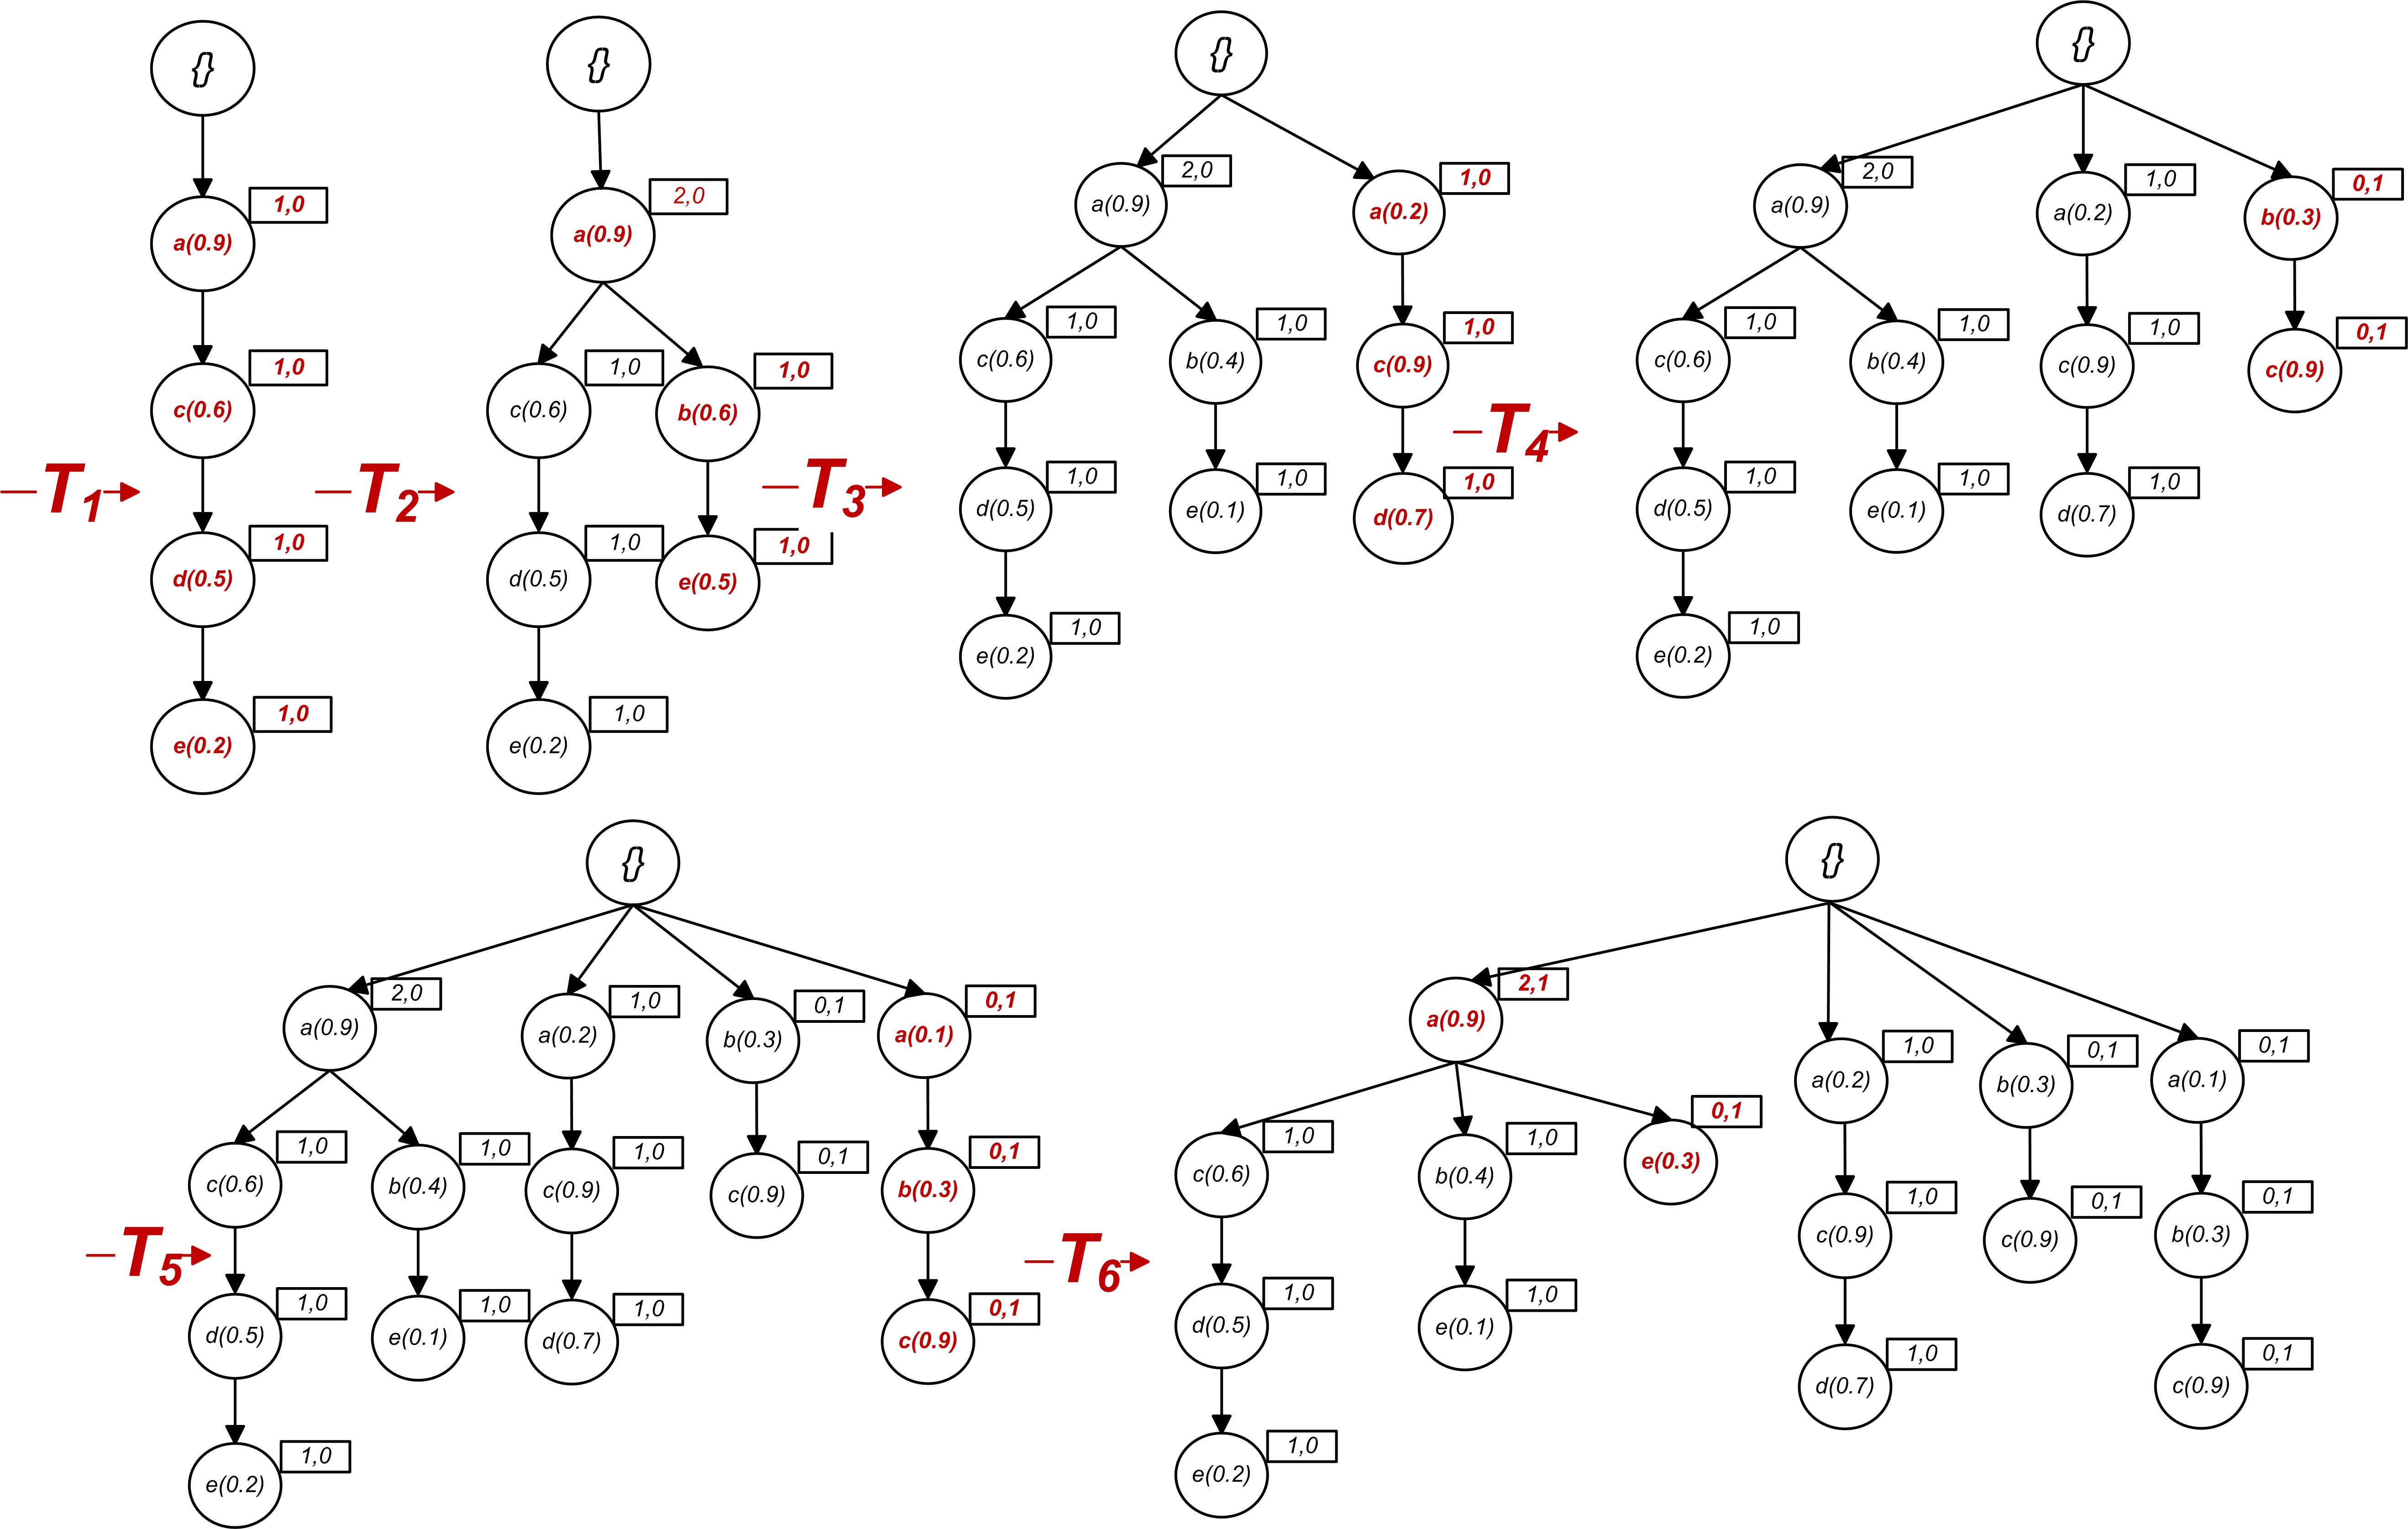
\includegraphics[width=.45\textwidth]{images/suf_simulation}
        \caption{SUF-growth ~\cite{suf_growth} tree construction}
        \label{figure:suf_simulation}
        \end{figure}
Considering the advantages of SUF-growth over others algorithm, there is the question. The is how SUF-growth ~\cite{suf_growth} algorithm find frequent item-sets from streams of uncertain data using a new tree structure called SUF-tree. Now we describe this. We first construct an SUF-tree, and then extract relevant paths from this SUF-tree (which is a global tree) to recursively from smaller UF-trees for projected databases. Due to the dynamic nature and Property 2 of data streams, expected the support of items is continuously affected by the arrival of new batches (and the removal of the contents of older batches). Arranging items in the frequency-dependent order in the SUF-tree may lead to swapping which, in turn, can cause merging and splitting—off tree nodes when the global frequencies of items change. Hence, in the SUF-tree, items are arranged according to some canonical order (e.g. lexicographic order), which can be specified by the user prior to the construction of the SUF-tree or the mining process. Consequently, the SUF-tree can be constructed using only one scan of the streams of uncertain data, and the resulting SUF-tree captures the contents of the streams. Moreover, the SUF-tree preserves the usual tree properties. The occurrence count of a node is at least as high as the sum of occurrence counts of its children.The ordering of items is unaffected by the continuous changes in the expected support values of items.

For example for table-\ref{table:uncertain_stream_transaction} transaction database let construct the SUF-tree. Figure-\ref{figure:suf_simulation} shows the construction of the SUF-tree. Here as the stuff tree is based on UF-tree construction approach the node sharing is very rare. From figure-\ref{figure:suf_simulation} it’s clearly visible that the node sharing is not that much impressive as the node should be shared if the two same item has same existential probability and in real life scenario this sharing is very rare. For this reason \emph{a(0.9)} in \emph{T\textsubscript{1}} and \emph{a(0.2)} in \emph{T\textsubscript{3}} did not share single node and the tree compactness could not be accomplished. Although the SUF-growth has resolved some limitations of UF-streaming ~\cite{suf_growth}, some limitations still exist. Tree structure it uses is UF-tree ~\cite{uf_growth} structure which suffers from compactness. So SUF-growth tree also inherits this limitation, tree construction cost will be much more (both running time and memory) as the transaction grows, mining algorithm it uses is FP-growth like the approach that generates a huge candidate sub-pattern tree that costs much in the mining time. It increased mining cost (both running time and memory).
    
\section{Our Proposed Approach}
For stream property, we will always lose data after data stream has flown away. To resolve this, we will propose a sliding window based approach, where we will keep the most recent information in a tree structure as the most recent data is most valuable. Later we will show how the window will slide, remove old data and insert new data in the tree. As, for uncertain data stream each same item in the different transaction has different existential probability, it becomes very difficult to merge (share) these nodes in the tree. This uncertainty property of item makes the tree huge. We have proposed a new \emph{U\textsuperscript{cap}} value for each item that helps to share a single node when constructing the tree which we named as \emph{US-tree}. We will show that our proposed tree \emph{US-tree} will be very compact and very efficient for later mining. Later, we will describe an approach for mining the \emph {US-tree} named \emph{USFP-growth} which is \emph{FP-growth} like approach. Later we will propose a method for filtering and removing false positives generated by our approach in the most probable candidate frequent patterns.



\subsubsection{Preliminaries}
    \paragraph{Batch and Window: }
    A group of consecutive transactions from a transaction \emph{DB}inserted in \emph{US-tree} at a time. Let table-\ref{table:uncertain_stream_transaction} batch size = \emph{3}. \emph{T\textsubscript{1}, T\textsubscript{2}, T\textsubscript{3}} is one batch and its batch-1. Then next three \emph{T\textsubscript{4}, T\textsubscript{5}, T\textsubscript{6}} is one batch and its batch-2. Window is the size of consecutive batchs one \emph{US-tree} can hold. Let table-\ref{table:transaction_batch} be an example of grouped transaction and batch number tagged. So for window size \emph{2} The in a certain time batch-1 and batch-2 will create a window. Then after some times when batch-3 comes then batch-2 and batch-3 will create the next window.
    
    \paragraph{U\textsuperscript{cap}: }
    The following equation is for \emph{U\textsuperscript{cap}} calculation.
    %\documentclass{article}
%\usepackage{amsmath}
%\begin{document}
\begin{equation}\label{equation:cap}
\text{\emph{U\textsuperscript{cap}}}(X_r) =\begin{cases}
				P(X_1), & \text{if $ h = 1$}\\
				P(X_r)*M, & \text{if $ h > 1$}
             
\end{cases}
where,\\ M=max_{1\leq q\leq h}P(X_q)
\end{equation}
%\end{document}
    For transaction \emph{DB} example in table-\ref{table:uncertain_stream_transaction} for \emph{T\textsubscript{1}}, \emph{U\textsuperscript{cap}} of \emph{a{0.9}} is $0.9$ as a is the first item. For \emph{c(0.6)} \emph{U\textsuperscript{cap}} is $0.9*0.6=0.45$, \emph{d(0.50)} \emph{U\textsuperscript{cap}} is $0.9*0.5=0.45$ and \emph{e(0.2)} \emph{U\textsuperscript{cap}} is $0.9*0.2=0.18$. \emph{U\textsuperscript{cap}} is the upper bound of existential probability. As we are taking the max of all previous items coming in a particular order all items or item sets having existential probability must be less than or equal \emph{U\textsuperscript{cap}}. that is $\forall(i,j)\{ P(I_i)*P(I_j)\leq U_{cap}(I_j)\}$ where $i < j$. So support must be less than or equal \emph{U\textsubscript{cap}}.
    Calculated \emph{U\textsuperscript{cap}} should be the upper bound of two item's existential probability because we have taken the maximum value of item that has come earlier. So, by two item set support that can have maximum support value, is \emph{U\textsuperscript{cap}} value. Item set having \emph{U\textsuperscript{cap}} less than minimum support must frequent. Though this may cause some false positives but it is for sure that no false negative will insert into this. 
  %\documentclass{article} 
%\usepackage{graphicx}  
%\usepackage{multirow}
%\usepackage[table]{xcolor}
%\usepackage{fixltx2e}
%\usepackage{array}
%
%\begin{document}
\begin{table}[t]
\centering

\begin{tabular}{|c|c|c|c|c|c|}
\hline
& No & \multicolumn{4}{c|}{Items in Transaction} \\ \hline \hline
\multirow{3}{*}{Batch 1}	&	T\textsubscript{1} & a(0.9) & c(0.6) & d(0.5) & e(0.2)\\
							&	T\textsubscript{2} & a(0.9) & b(0.4) & e(0.1) & --    \\
							&	T\textsubscript{3} & a(0.2) & c(0.9) & d(0.7) & --    \\\hline
\multirow{3}{*}{Batch 2}	&	T\textsubscript{4} & b(0.3) & c(0.9) & -- & --\\
							&	T\textsubscript{5} & a(0.1) & b(0.3) & c(0.9) & --    \\
							&	T\textsubscript{6} & a(0.9) & e(0.3) & -- & --        \\\hline
\multirow{3}{*}{Batch 3}	&	T\textsubscript{7} & a(0.1) & d(0.6) & e(0.2) & --    \\
							&	T\textsubscript{8} & a(0.1) & c(0.2) & f(0.6) & --    \\
							&	T\textsubscript{9} & c(0.2) & d(0.9) & f(0.6) & --    \\\hline
							
\multirow{3}{*}{Batch 4}	&	T\textsubscript{10} &  --  &  --  &  --  & --    \\
							&	T\textsubscript{11} &  --  &  --  &  --  & --    \\
							&	T\textsubscript{12} &  --  &  --  &  --  & --    \\\hline
\end{tabular}
\caption{Uncertain Stream Transaction Data Divided into Batch}
\label{table:transaction_batch}
\end{table}


%
%\end{document}
      
Our proposed algorithm is divided into five steps. (1) Grouping transactions into batches and window and giving each item in a transaction a prefix value is called \emph{U\textsuperscript{cap}}. (2) Insert transaction into \emph {US-tree}. (3) Sliding the \emph {US-tree} (4) mining the \emph {US-tree} with \emph{USFP-growth} algorithm and (5) Eliminating false positive (not frequent but exists infrequent item set) . For simulating our approach we consider Table~\ref{table:uncertain_stream_transaction} as uncertain stream transaction data. For this simulation, we consider window size as 2 and batch size 3. That means 3 transactions creates a batch and 2 batches create a window. After completing window construction (inserting batch 1 and 2), the \emph {US-tree} will be full. When new batch comes we slide the window. That means we remove oldest batch batch-1 and put batch-2 as the old batch. Then insert new batch in the tree as batch-3. So for window size 2 the tree always contains at most 2 batches. Thus, the tree always holds the latest information. In next subsections, we will elaborately explain our approach of every step.



\subsubsection{Preparation}

 %\documentclass{article} 
%\usepackage{graphicx}  
%\usepackage{multirow}
%\usepackage[table]{xcolor}
%\usepackage{fixltx2e}
%\usepackage{array}
%
%\begin{document}
\begin{table}
\centering

\begin{tabular}{|c|c|c|c|c|c|}
\hline
	Batch No& Transaction No & \multicolumn{4}{c|}{Items in Transaction} \\ \hline \hline
	\multirow{3}{*}{Batch 1}	&	T\textsubscript{1} & a(0.9) & c(0.54) & d(0.45) & e(0.18)		\\
								&	T\textsubscript{2} & a(0.9) & b(0.36) & e(0.09) & --			\\
								&	T\textsubscript{3} & a(0.2) & c(0.18) & d(0.63) & --			\\\hline
	\multirow{3}{*}{Batch 2}	&	T\textsubscript{4} & b(0.3) & c(0.27) & --  	& --			\\
								&	T\textsubscript{5} & a(0.1) & b(0.03) & c(0.27) & --  			\\
								&	T\textsubscript{6} & a(0.9) & e(0.27) & --	    & --  			\\\hline
	\multirow{3}{*}{Batch 3}	&	T\textsubscript{7} & a(0.1) & d(0.06) & e(0.12) & --			\\
								&	T\textsubscript{8} & a(0.1) & c(0.02) & f(0.12) & --   			\\
								&	T\textsubscript{9} & c(0.2) & d(0.09) & f(0.54) & --   			\\\hline
								
	\multirow{3}{*}{Batch 4}	&	T\textsubscript{10} &  --  &  --  &  --  & --    				\\
								&	T\textsubscript{11} &  --  &  --  &  --  & --    				\\
								&	T\textsubscript{12} &  --  &  --  &  --  & --    				\\\hline
	\end{tabular}
\caption{Window and Batch of Table \ref{table:uncertain_stream_transaction}}
\label{table:prefix_assigned}
\end{table}


%
%\end{document}
    In this section we will describe the batch and window grouping and the prefix value \emph{U\textsuperscript{cap}} calculation. First we calculate batch and window calculation and grouping our transaction data. As we describe earlier for the example Table-\ref{table:uncertain_stream_transaction} easy simulation we take batch size as \emph{$3$} and window size as \emph{$2$}. So first \emph{$3$} transactions \emph{T\textsubscript{1}}, \emph{T\textsubscript{2}} and \emph{T\textsubscript{3}} are grouped and labeled as \emph{Batch-1}. Then next \emph{$3$} \emph{T\textsubscript{4}}, \emph{T\textsubscript{5}} and \emph{T\textsubscript{6}} are grouped together and labeled as \emph{Batch-2}. Next \emph{$3$} \emph{T\textsubscript{7}}, \emph{T\textsubscript{8}} and \emph{T\textsubscript{9}} are grouped together and labeled as \emph{Batch-3}. Thus the consecutive next \emph{$3$} transaction should be grouped as batch and ready to be inserted into \emph{US-tree}. As our window size is $2$, after inserting two batches into the \emph{US-tree} the window will be completed. Before inserting next batch \emph{Batch-3} we need to remove \emph{Batch-1}(oldest one) from tree and move \emph{Batch-2} to \emph{Batch-1 's} position and then insert new batch, \emph{Batch-3}. Thus the latest information is inserted and kept into the \emph{US-tree}. table-\ref{table:transaction_batch} shows the window and batch grouped for stream transaction example table-\ref{table:uncertain_stream_transaction}.
    For this calculation we earlier proposed an equation-\ref{equation:cap}. From this equation we can create \emph{U\textsuperscript{cap}} for each item in a transaction. To calculate one transaction, for each item in a transaction, if item is the first item in a transaction than item's existential probability is its \emph{U\textsuperscript{cap}} value, otherwise item's \emph{U\textsuperscript{cap}} is max of previous items existential probability multiplied by item's  own existential probability. For example, let Table-\ref{table:transaction_batch} T1 is \emph{a(0.9), c(0.6), d(0.5), e(0.2)}. 
  
In this transaction item \emph{a(0.9)} is the first item. So its \emph{U\textsuperscript{cap}} is 0.9.

For second item, \emph{c(0.60)} previous item is only \emph{a(0.90)}. So c's $\emph{U\textsuperscript{cap}} = 0.9*0.6 = 0.54$.

For third item, \emph{d(0.50)} there are two items before it, \emph{a(0.9)} and \emph{c(0.6)}. Among them \emph{a} has max existential probability, that is \emph{0.9}. So \emph{d's } $\emph{U\textsuperscript{cap}} = 0.9*0.5 = 0.45$.

For fourth item \emph{e(0.2)} there are three items before it, \emph{a(0.9)} ,\emph{c(0.6)} and \emph{d(0.5)}. Among them \emph{a} has max existential probability is \emph{0.9}. So \emph{e's}  $\emph{U\textsuperscript{cap}} = 0.9*0.2 = 0.45$. Thus we can calculate each item's \emph{U\textsuperscript{cap}} value for a transaction. For easier understanding we have calculated all the item's \emph{U\textsuperscript{cap}} of Table-\ref{table:transaction_batch} and put into Table-\ref{table:prefix_assigned}.

\subsubsection{US-tree Construction}
As described earlier about our batch and window. A batch should be inserted into the tree in its own window slot. After inserting all batches, the window will be complete and be ready to mine. We said earlier section that our tree will be very compact. For this we have proposed an approach for sharing nodes. For sharing same tree nodes two items with same id and order should not care about own existential probability. If item is already in the tree with same id then two items should share the node. Thus the tree will be very compact. When inserting an item in the tree the \emph{U\textsuperscript{cap}} of the tree should be updated by adding the prefix value of the node. Thus each batch should be inserted into the tree.
    %\documentclass{article}
%\usepackage{graphicx}
%\usepackage{caption}
%\usepackage{subcaption}
%
%\begin{document}
\begin{figure}
  \centering
	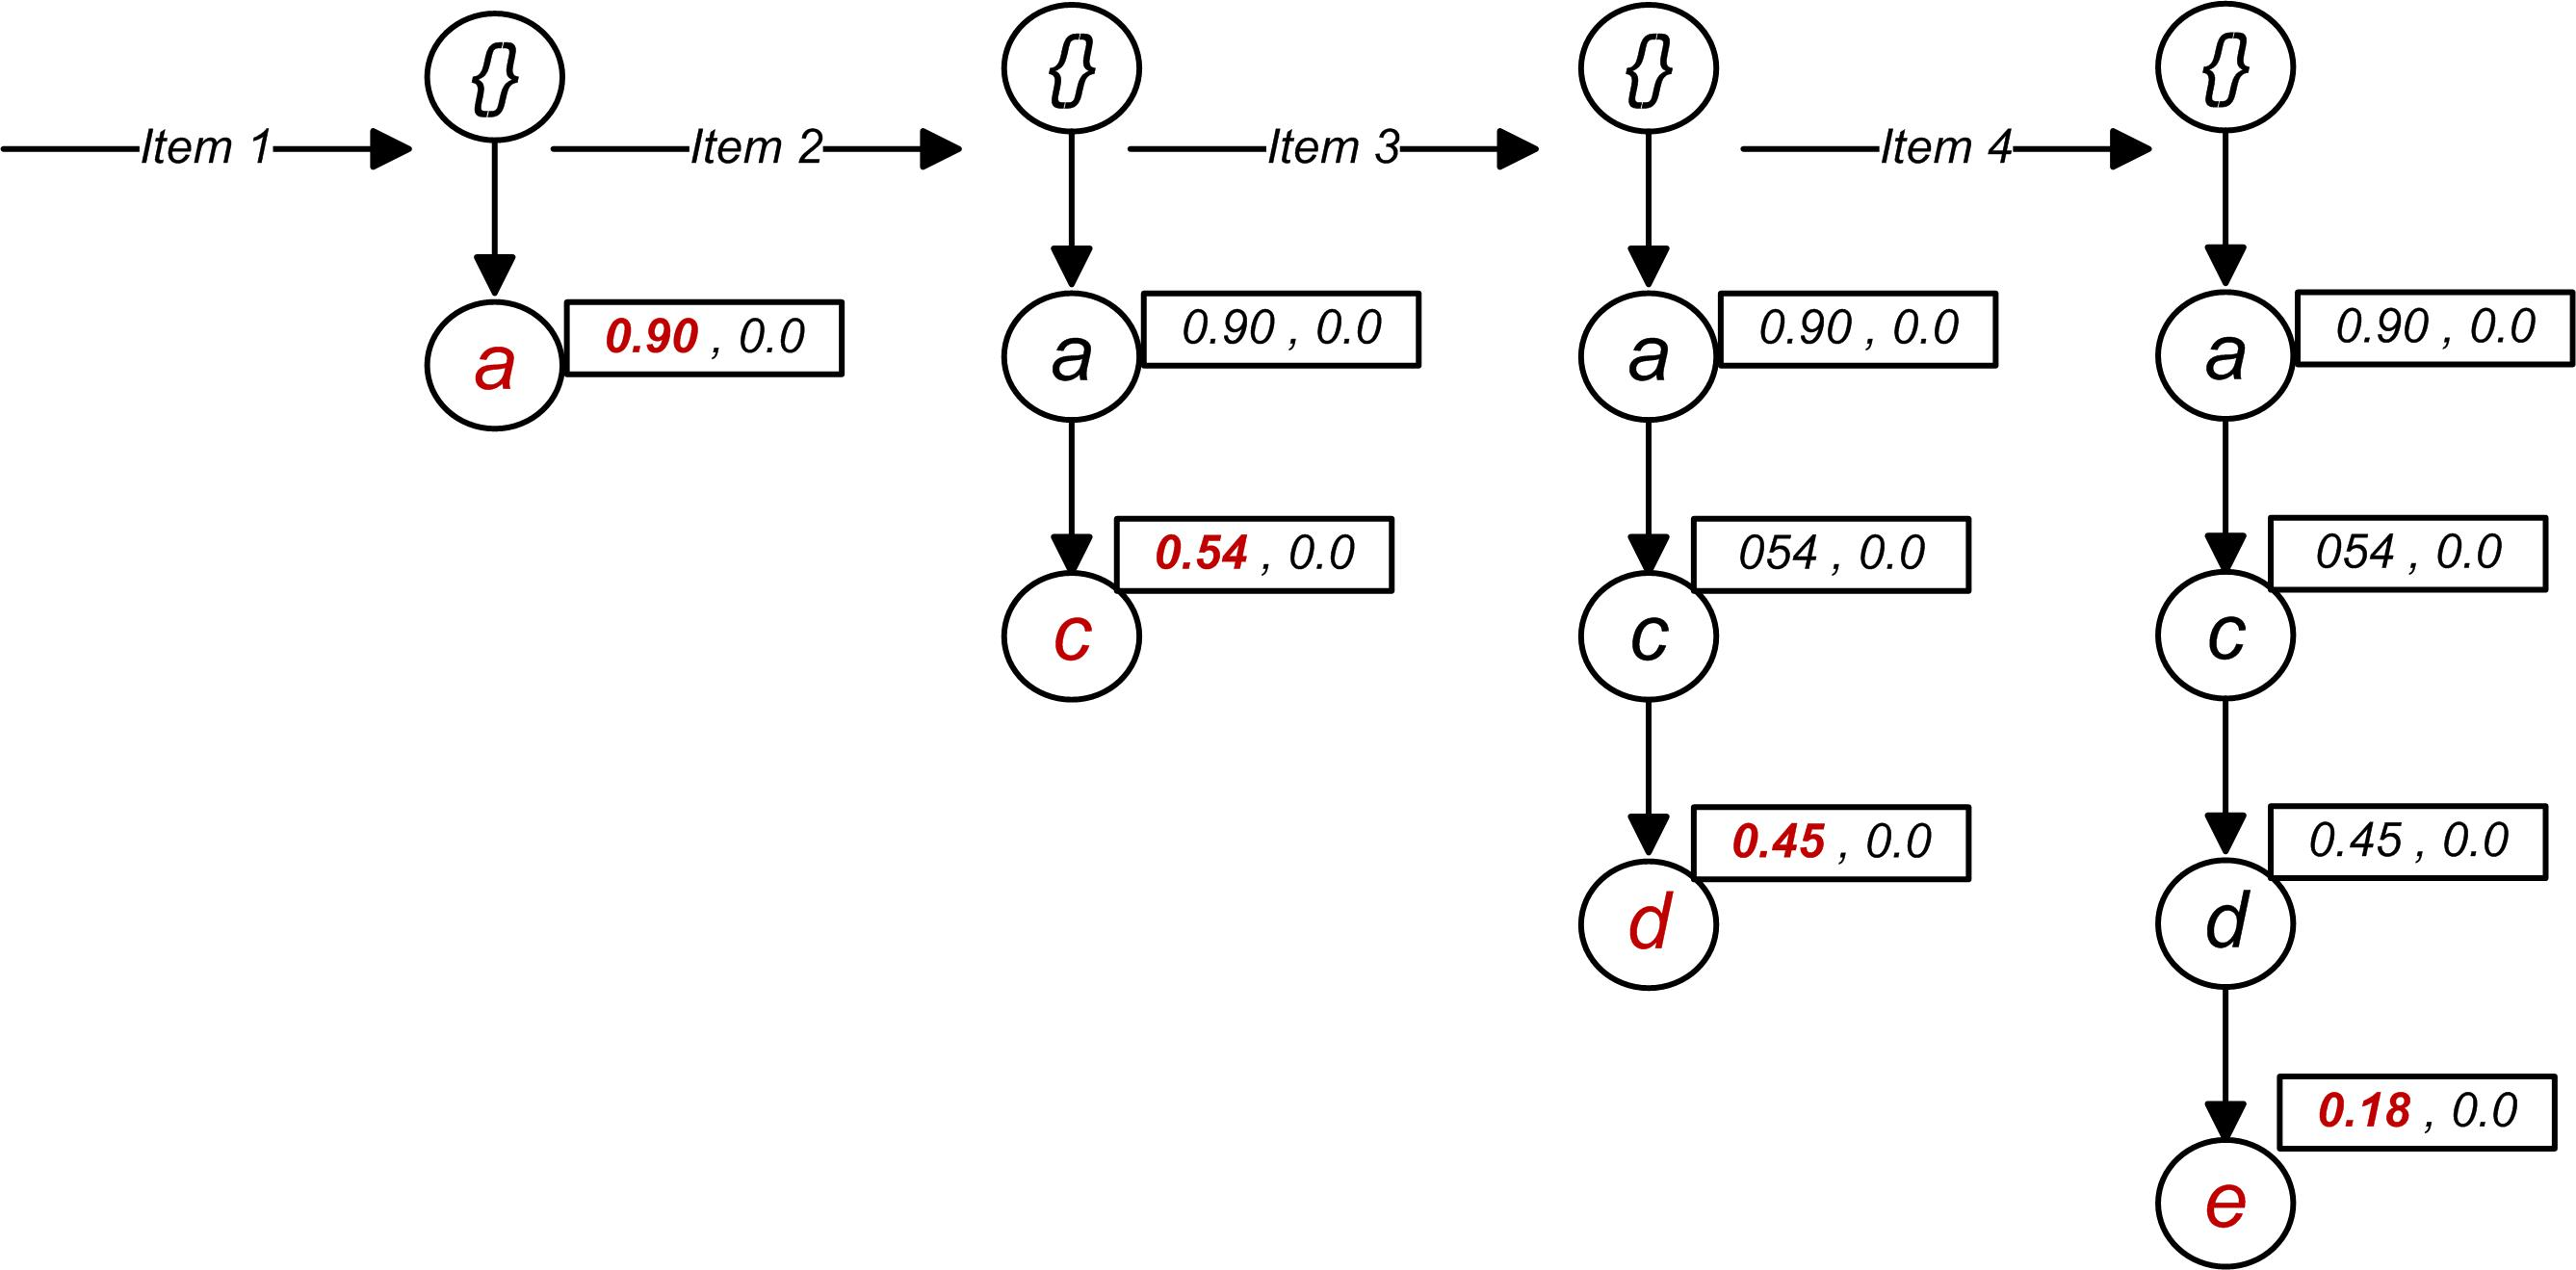
\includegraphics[width=.4\textwidth,height=5cm]{images/sim_01.jpg}  
	\caption{Inserting $T_1$ into US-tree}
	\label{figure:t1}
\end{figure}

\begin{figure}
\begin{minipage}{0.20\textwidth}
  \centering
  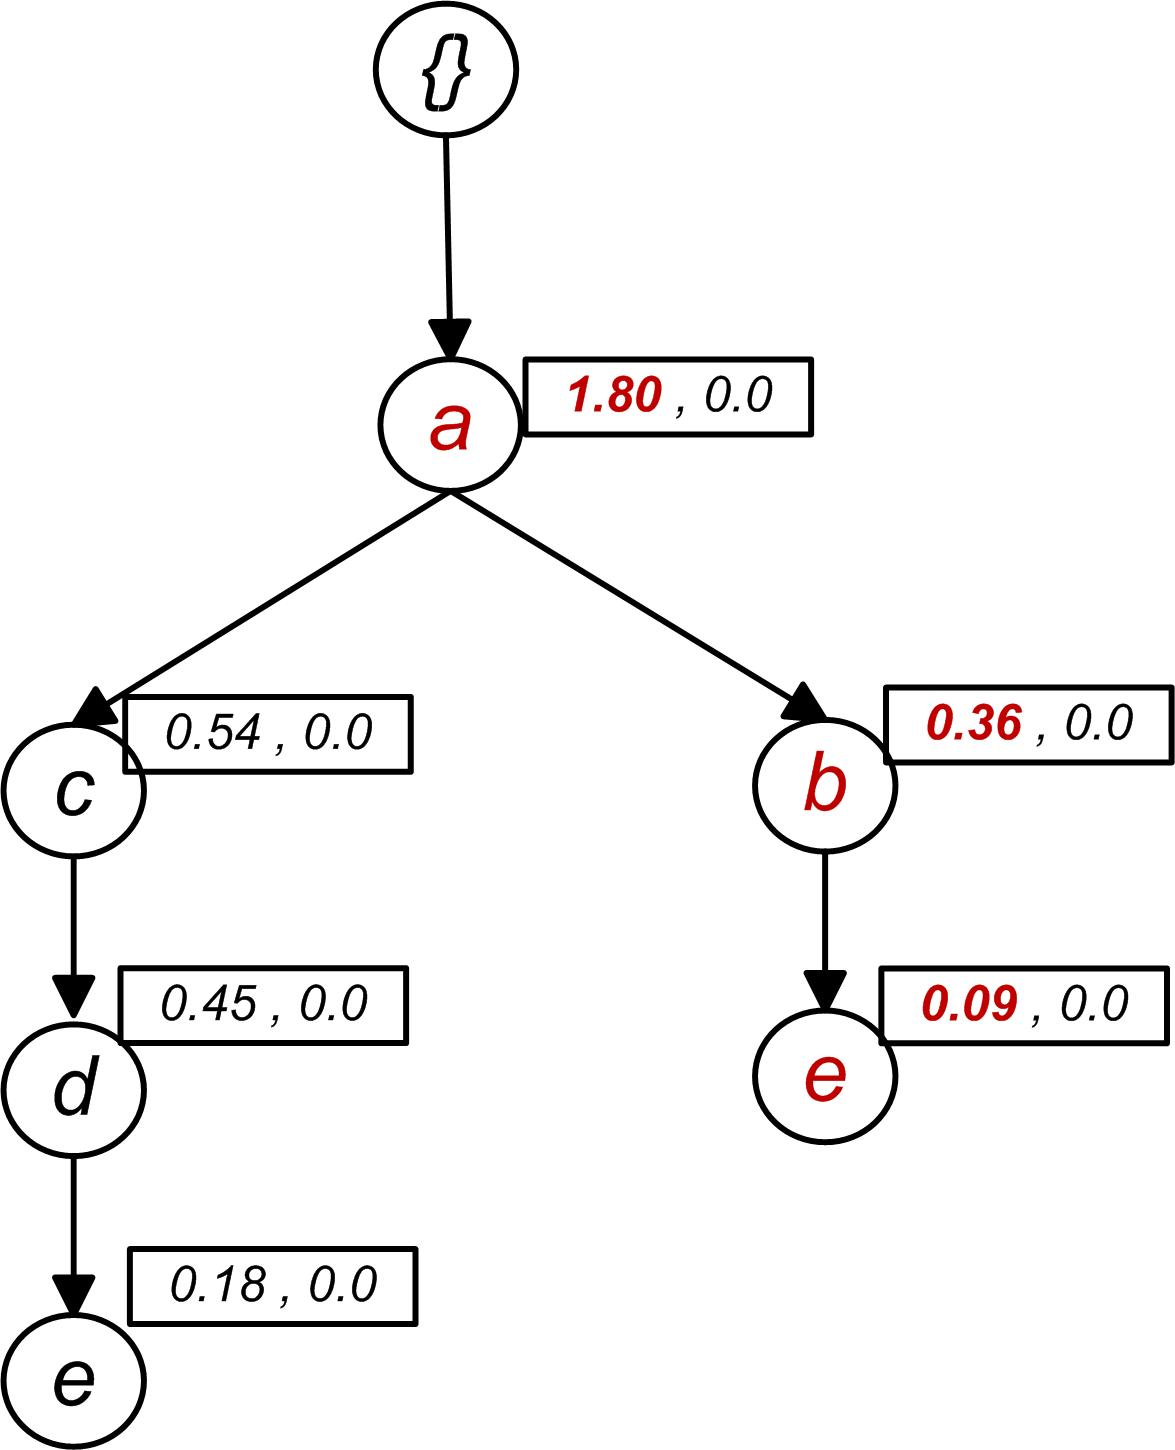
\includegraphics[width=\textwidth]{images/sim_02.jpg}
\end{minipage}
\hfill
\begin{minipage}{0.20\textwidth}
  \centering
  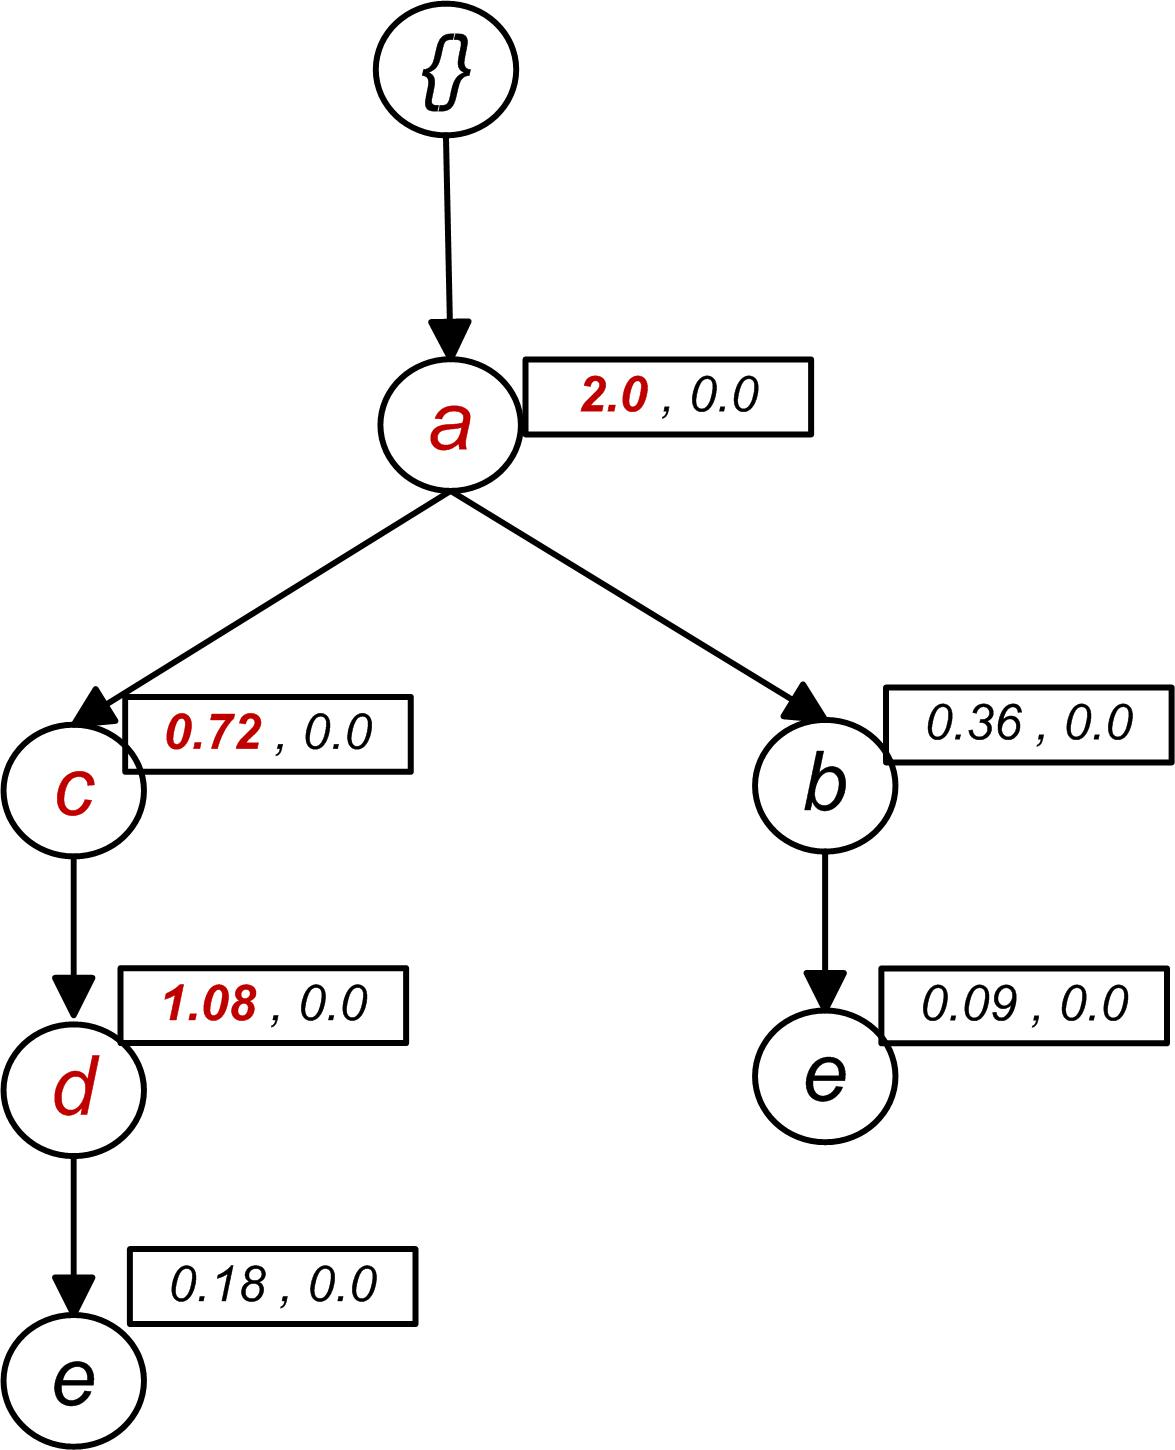
\includegraphics[width=\textwidth]{images/sim_03.jpg}
\end{minipage}
 \caption{Inserting $T_2$ and $T_3$ in US-tree}
 \label{figure:t23}
\end{figure}

\begin{figure}
\begin{minipage}{0.25\textwidth}
  \centering
  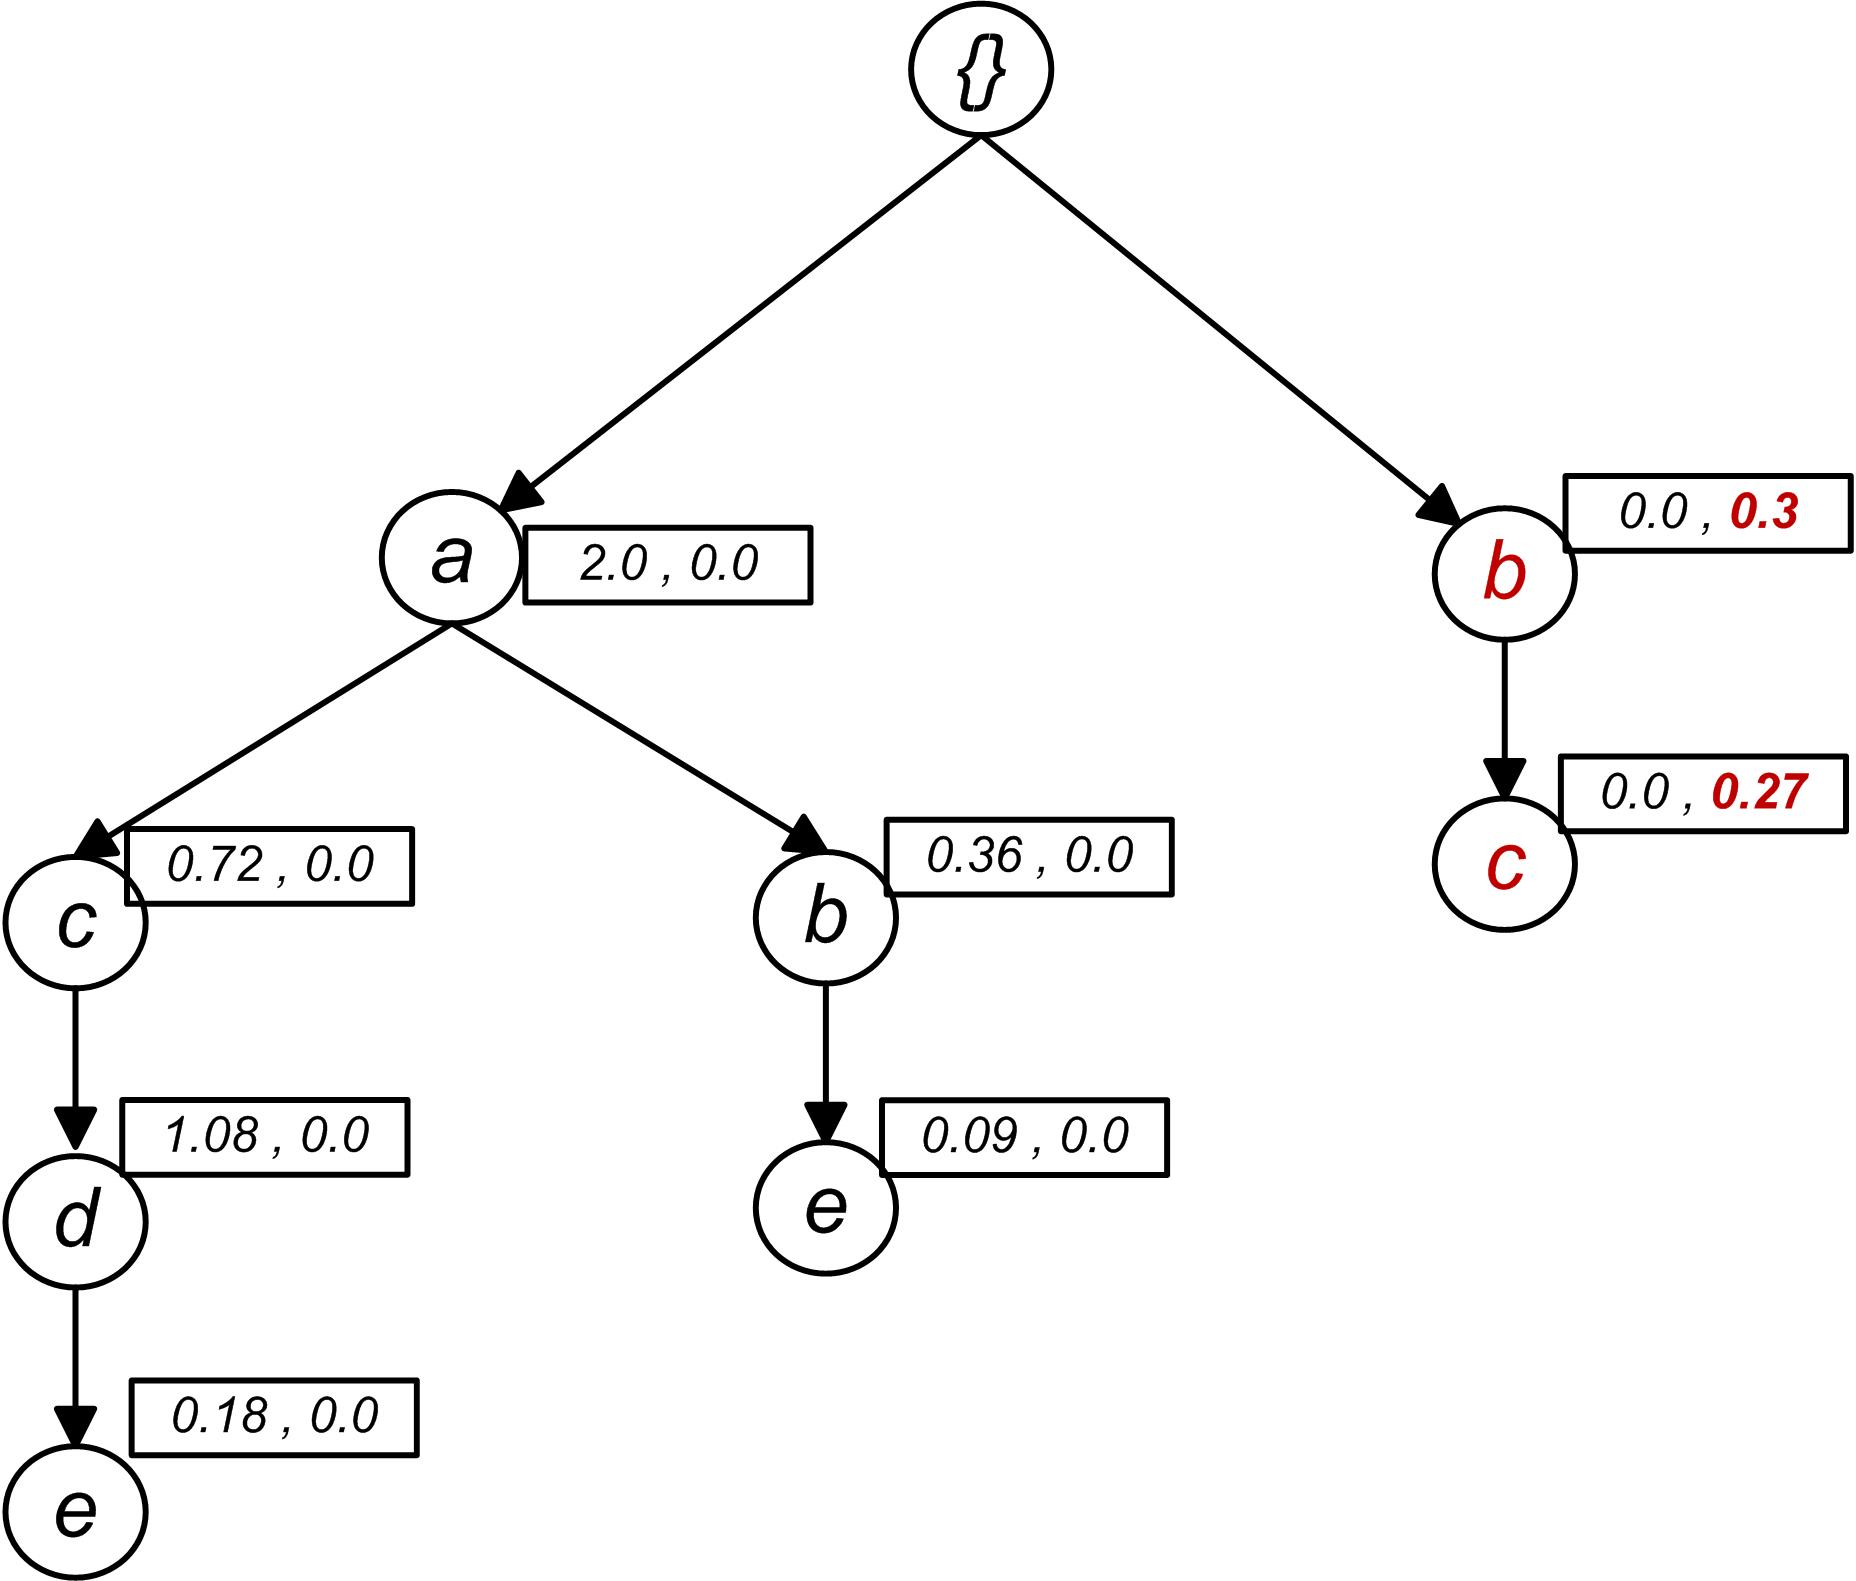
\includegraphics[width=\textwidth]{images/sim_04.jpg}
\end{minipage}
\hfill
\begin{minipage}{0.25\textwidth}
  \centering
  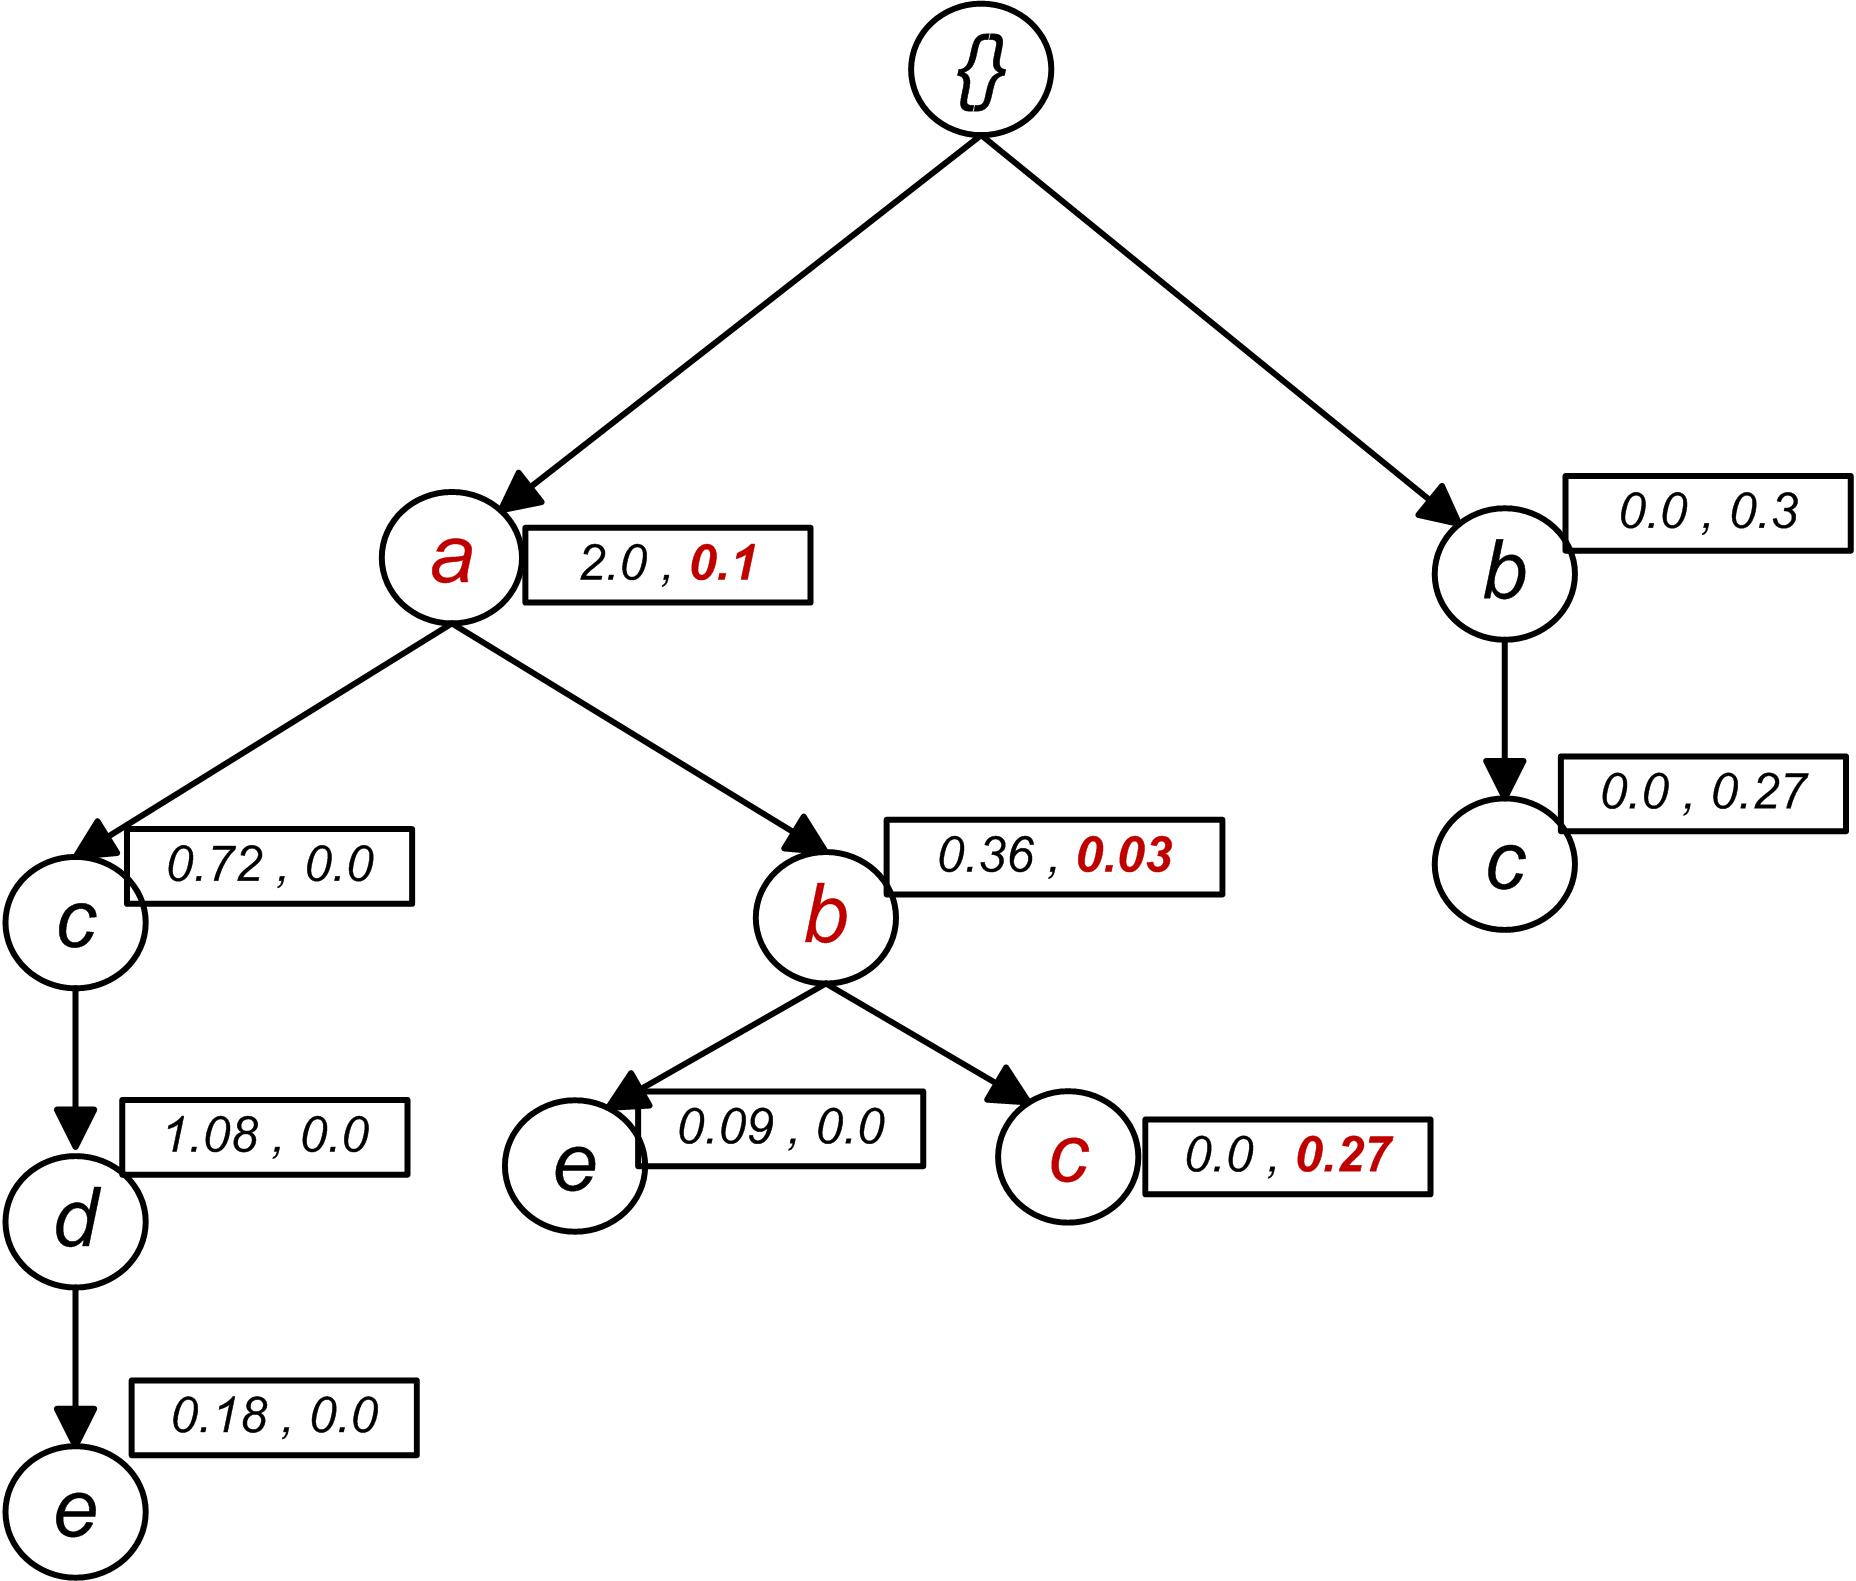
\includegraphics[width=\textwidth]{images/sim_05.jpg}
\end{minipage}
\caption{Inserting $T_4$ and $T_5$ in US-tree}
 \label{figure:t456}
\end{figure}


\begin{figure}
  \centering
	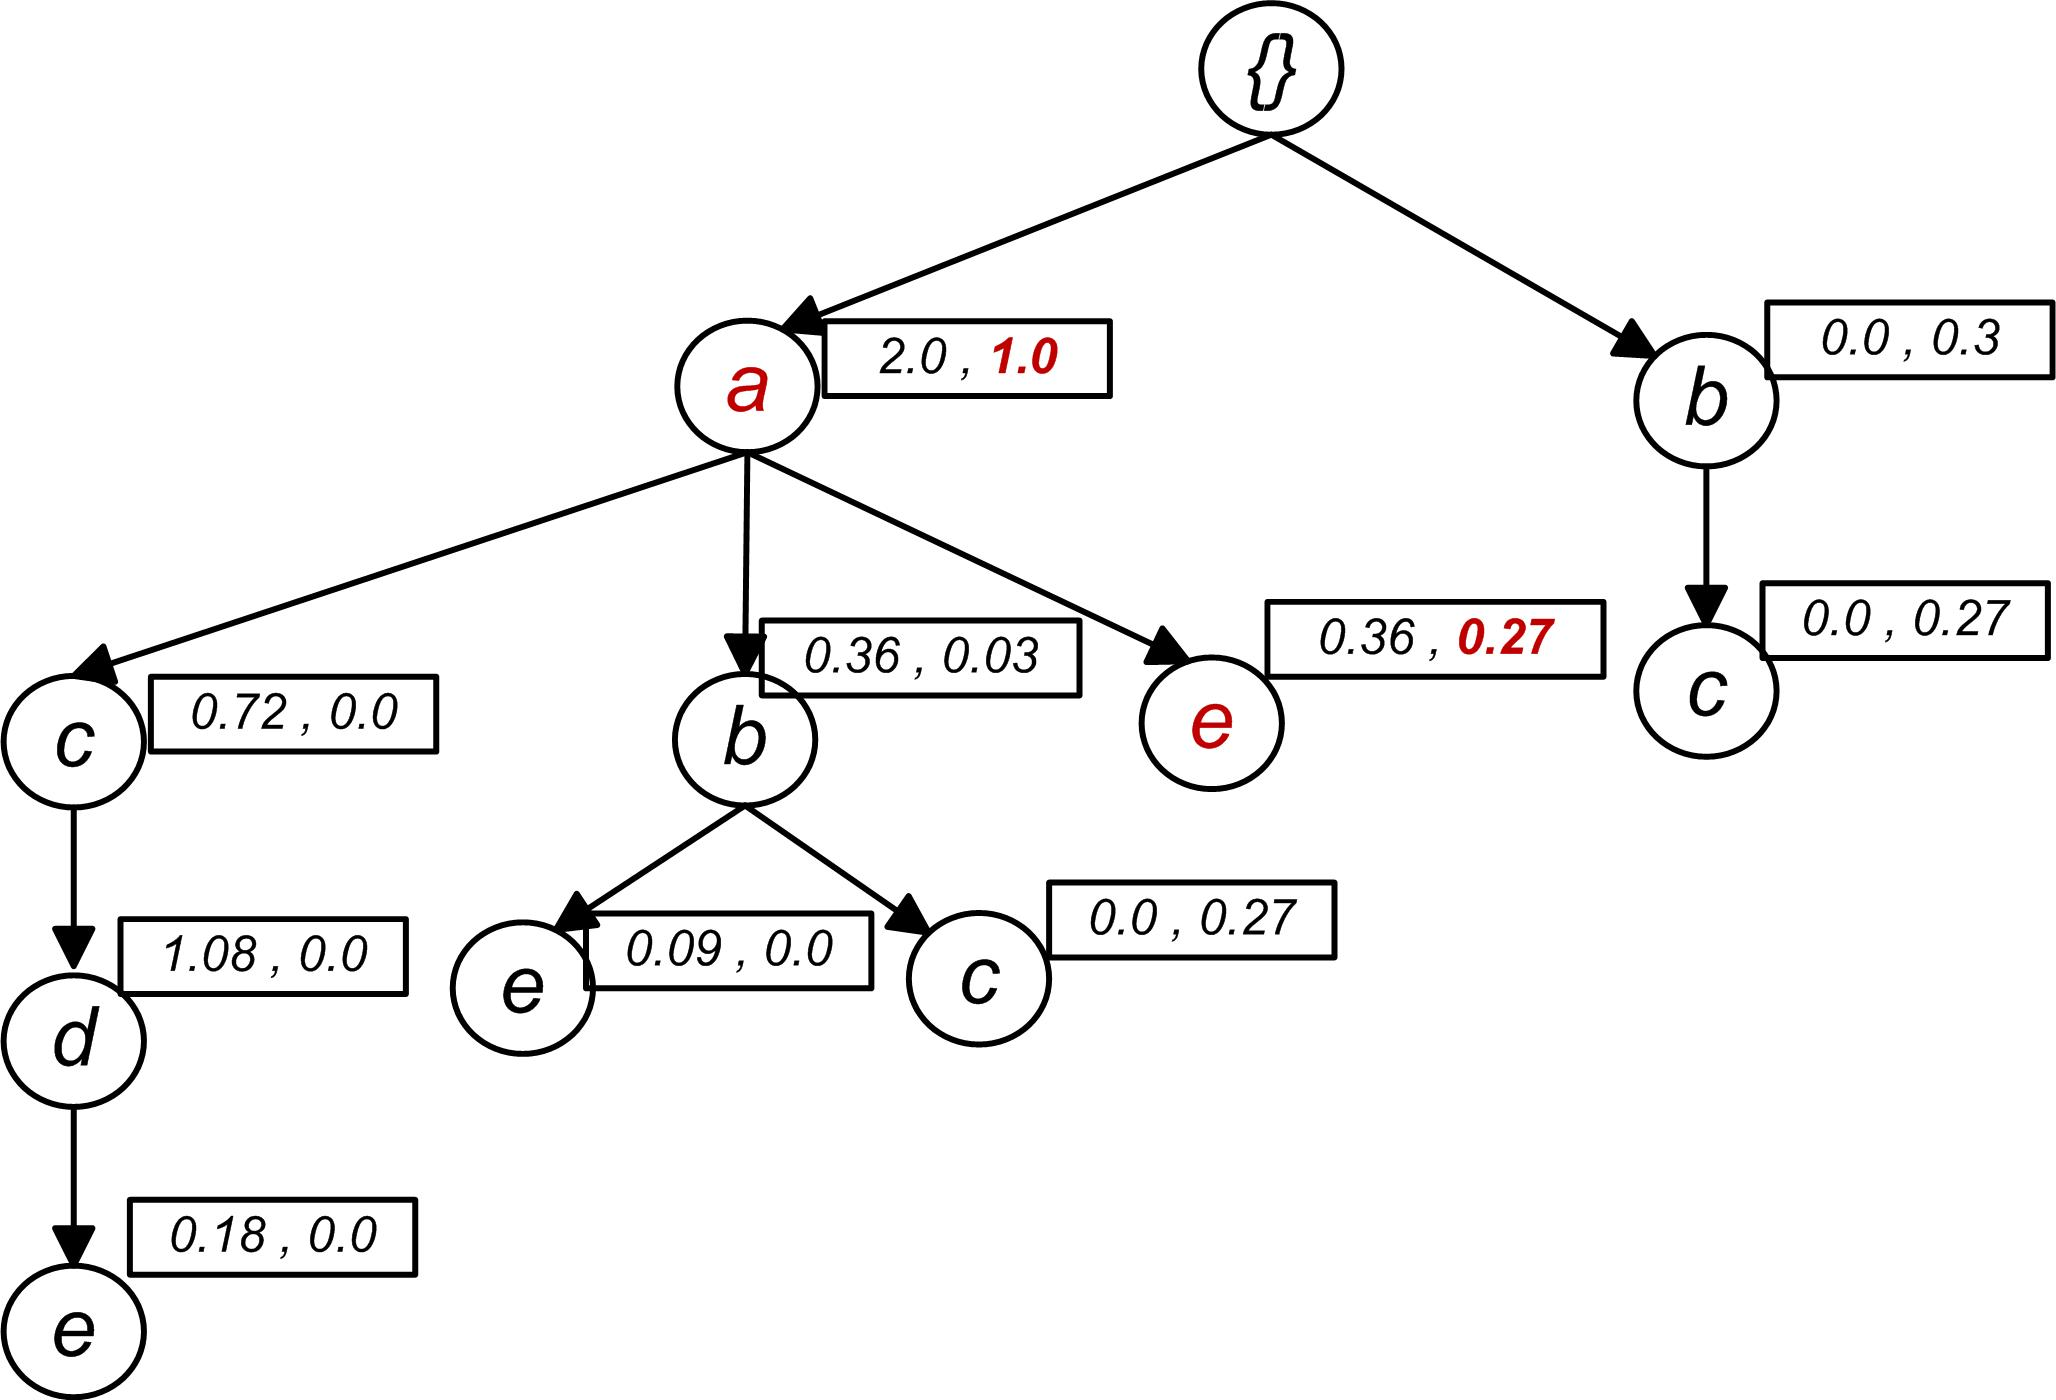
\includegraphics[width=.3\textwidth]{images/sim_06.jpg}  
	\caption{Inserting $T_6$ into US-tree}
	\label{figure:t6}
\end{figure}

%\begin{figure}
%\begin{minipage}{0.50\textwidth}
%  \centering
%  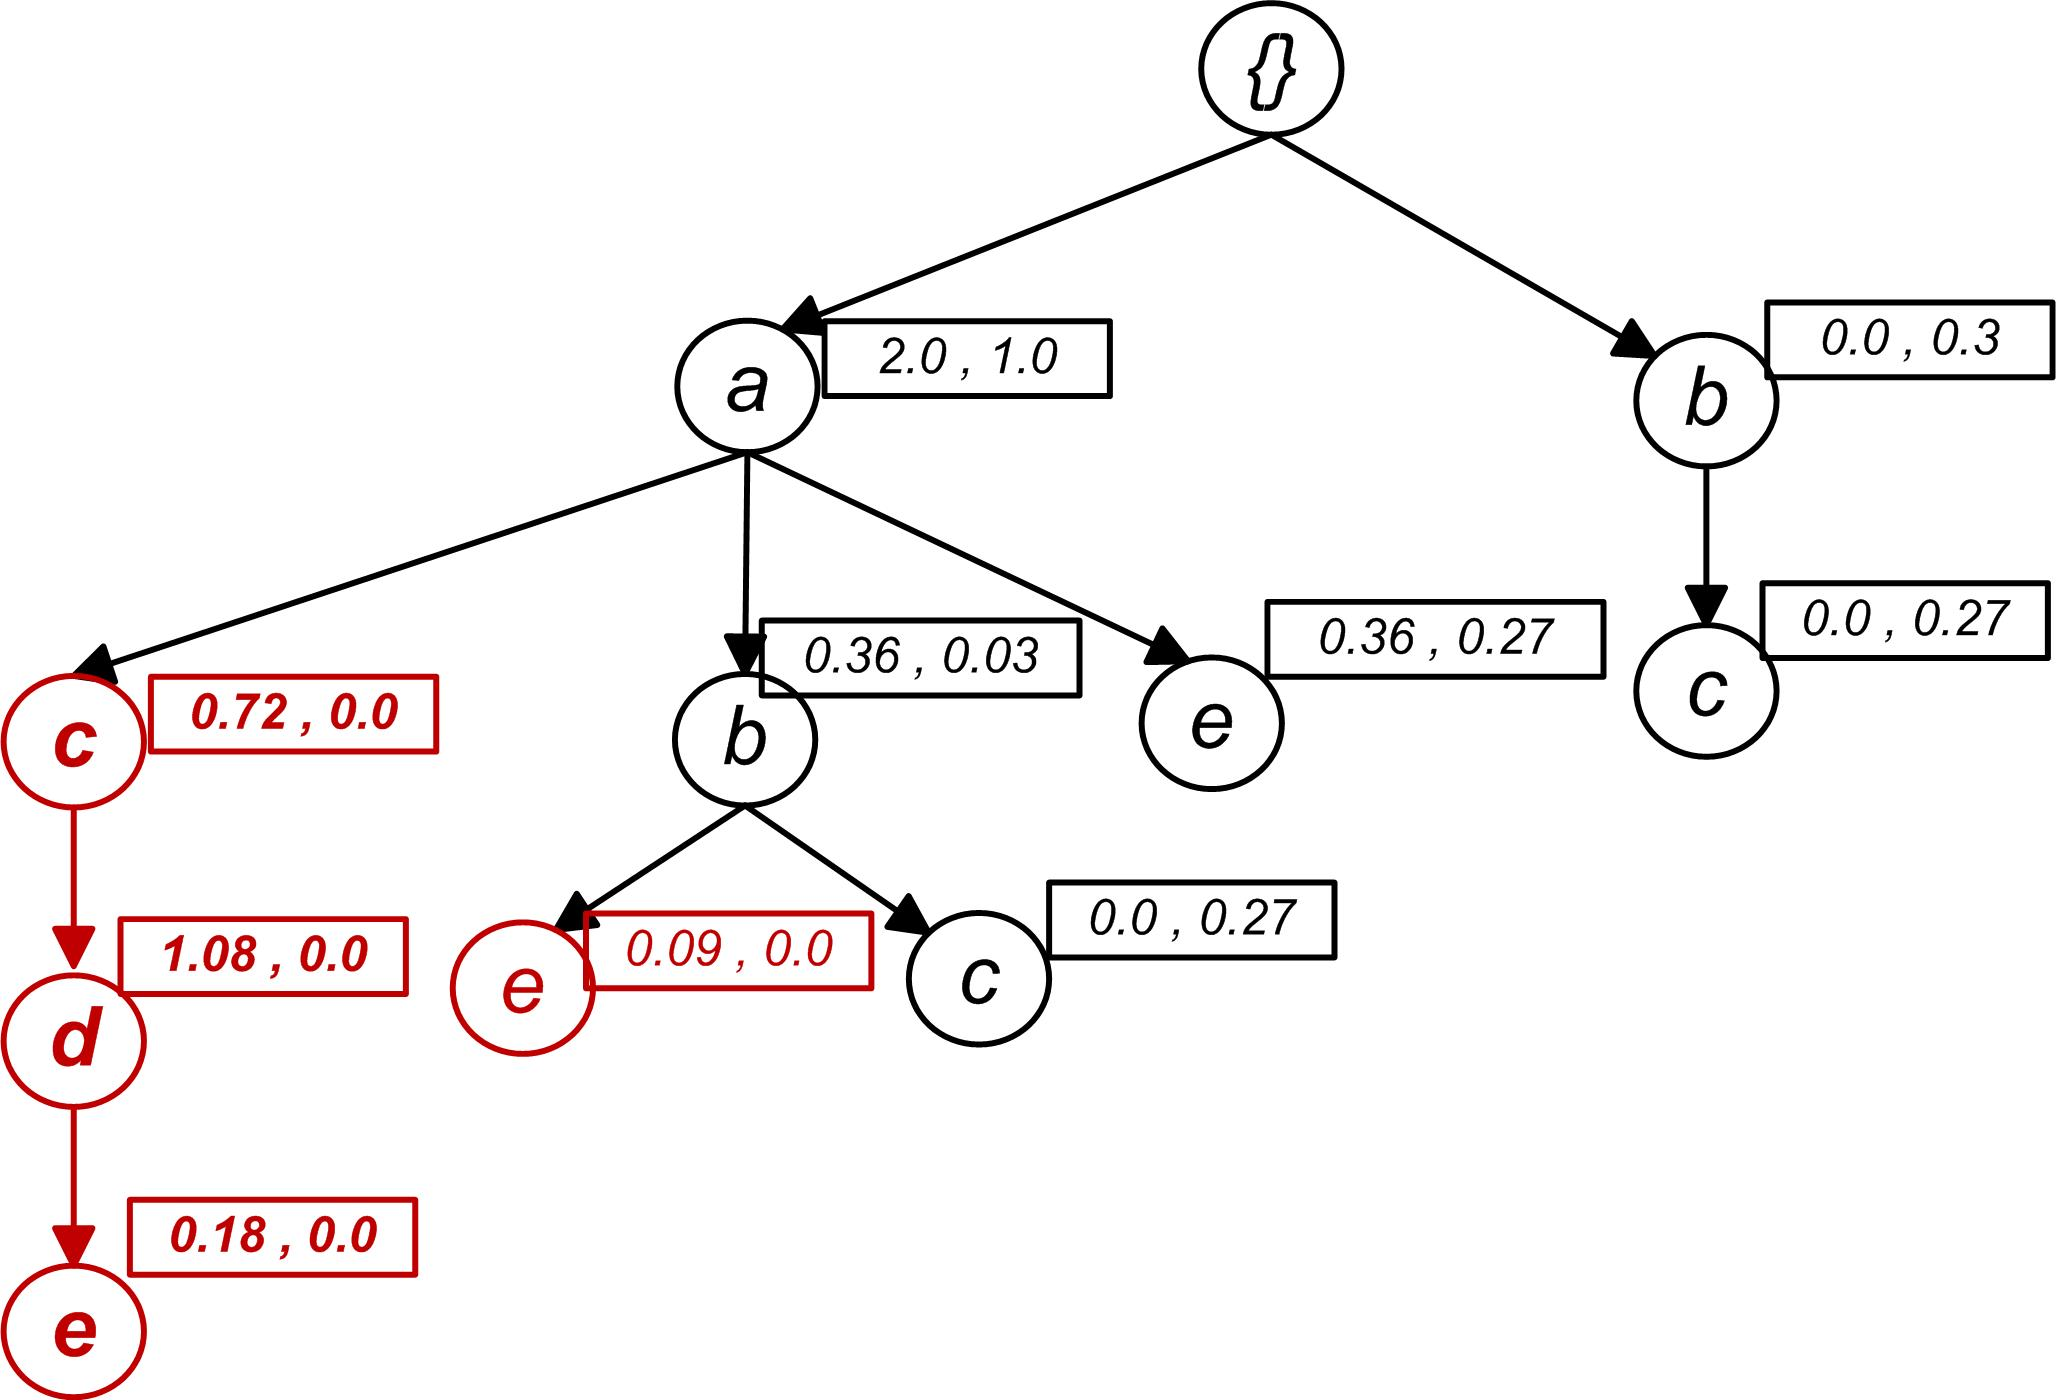
\includegraphics[width=\textwidth]{images/sim_06_slide.jpg}
%\end{minipage}
%\hfill
%\begin{minipage}{0.50\textwidth}
%  \centering
%  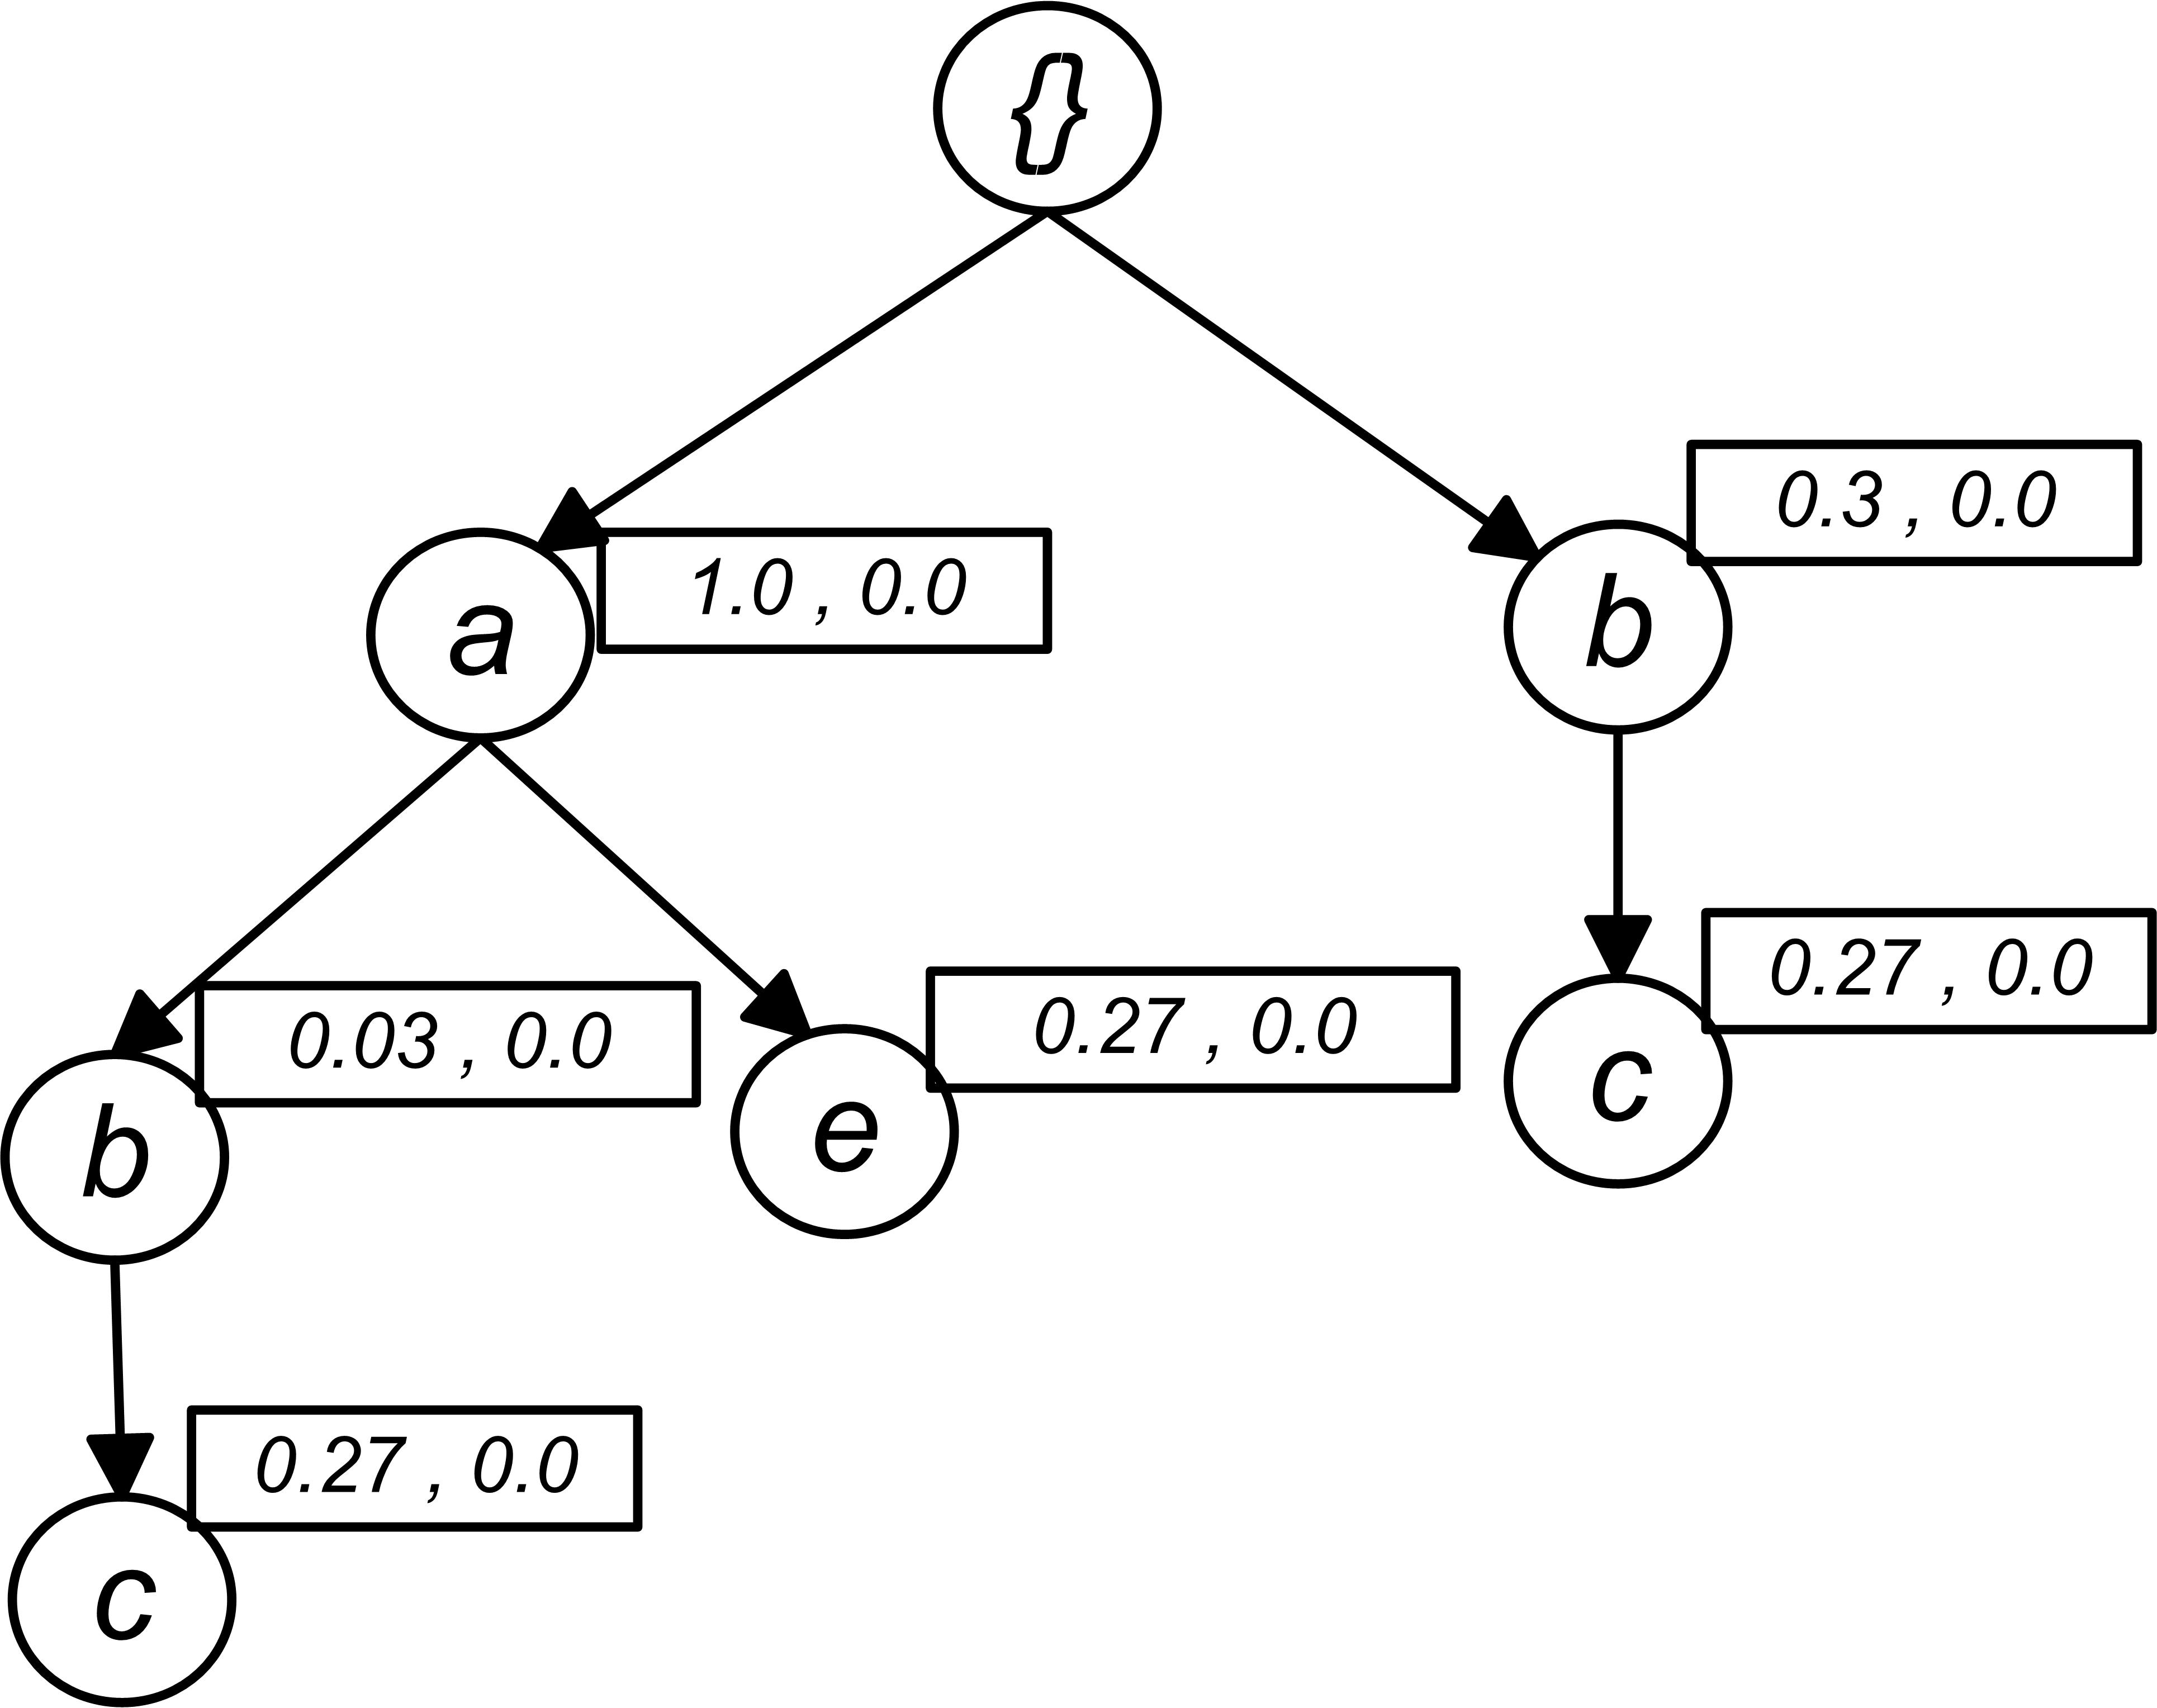
\includegraphics[width=\textwidth]{images/sim_06_slide_2.jpg}
%\end{minipage}
%\caption{Slide Window}
%\label{figure:frequent_patterns_final}
%\end{figure}
%\end{document}
    Let construct tree for Table-\ref{table:prefix_assigned}. First we insert \emph{Batch-1 (T\textsubscript{1}, T\textsubscript{2}, T\textsubscript{3})} in the window 1. First when inserting the \emph{T\textsubscript{1} - a(0.9), c(0.54), d(0.45), e(0.18)} we insert item \emph{a(0.9)} as a child of root \emph{\{\}} (Figure-\ref{figure:t1}). Update a's prefix value as $0.9$. Then we add \emph{c(0.54)} as a's child update c's prefix value as $0.54$. Aad \emph{d(0.45)} as c's child update d's prefix value as $0.45$. Add \emph{e(0.18)} as d's child update e's prefix value as $0.18$. Thus \emph{T1} is inserted into the tree (Figure-\ref{figure:t1}). For \emph{T\textsubscript{2} - a(0.9), b(0.36), e(0.09)} first we insert \emph{a(0.9)}. Here we found \emph{a} is already inserted so we just update existing node a's prefix value $0.9 + 0.9 = 1.8$ (Figure-\ref{figure:t23}). Then we insert \emph{b(0.36)}. As \emph{a} has no child \emph{b} we insert a new child b and update its prefix value $0.36$. Then insert new e(0.09) as the child of \emph{b}. For \emph{T\textsubscript{3} - a(0.2), c(0.18), d(0.63)} we follow the existing path \emph{a(1.8), c(0.54), d(0.45)} and update corresponding prefix value as $1.8 + 0.2 = 2.0$, $0.54 + 0.18 = 0.72$ and $0.45 + 0.63 = 1.08$ (Figure-\ref{figure:t23}). After inserting the This \emph{T\textsubscript{3}} window 1 is completed. Then we will go for inserting next batch \emph{Batch-2 (T\textsubscript{4}, T\textsubscript{5}, T\textsubscript{6})} in the tree. For \emph{Batch-2} we shall put prefix value in the window's newest place. And thus the latest batch becomes the most recent information. For inserting \emph{T\textsubscript{4} - b(0.3), c(0.27)} we insert new node \emph{b} as there is no child b of root node \emph{\{\}}. So we insert \emph{b} as a child of root \emph{\{\}}. Update its prefix value as $0.3$. Then insert \emph{c(0.27)} as child of \emph{b} and update prefix value $0.27$. Here as this \emph{T\textsubscript{4}} is inserting in \emph{Batch-4} we update prefix value for recent batch's information. Next we insert \emph{T\textsubscript{5} - a(0.1), b(0.03), c(0.27)}. We merge \emph{a(0.1), b(0.03)} with previous \emph{a, b } nodes and update prefix value $0.1$ and $0.03$ in the second batch's portion and insert new node \emph{b} as a child of \emph{b} and update its prefix value as $0.27$ (Figure-\ref{figure:t456}).
    \begin{figure}
\begin{minipage}{0.27\textwidth}
  \centering
  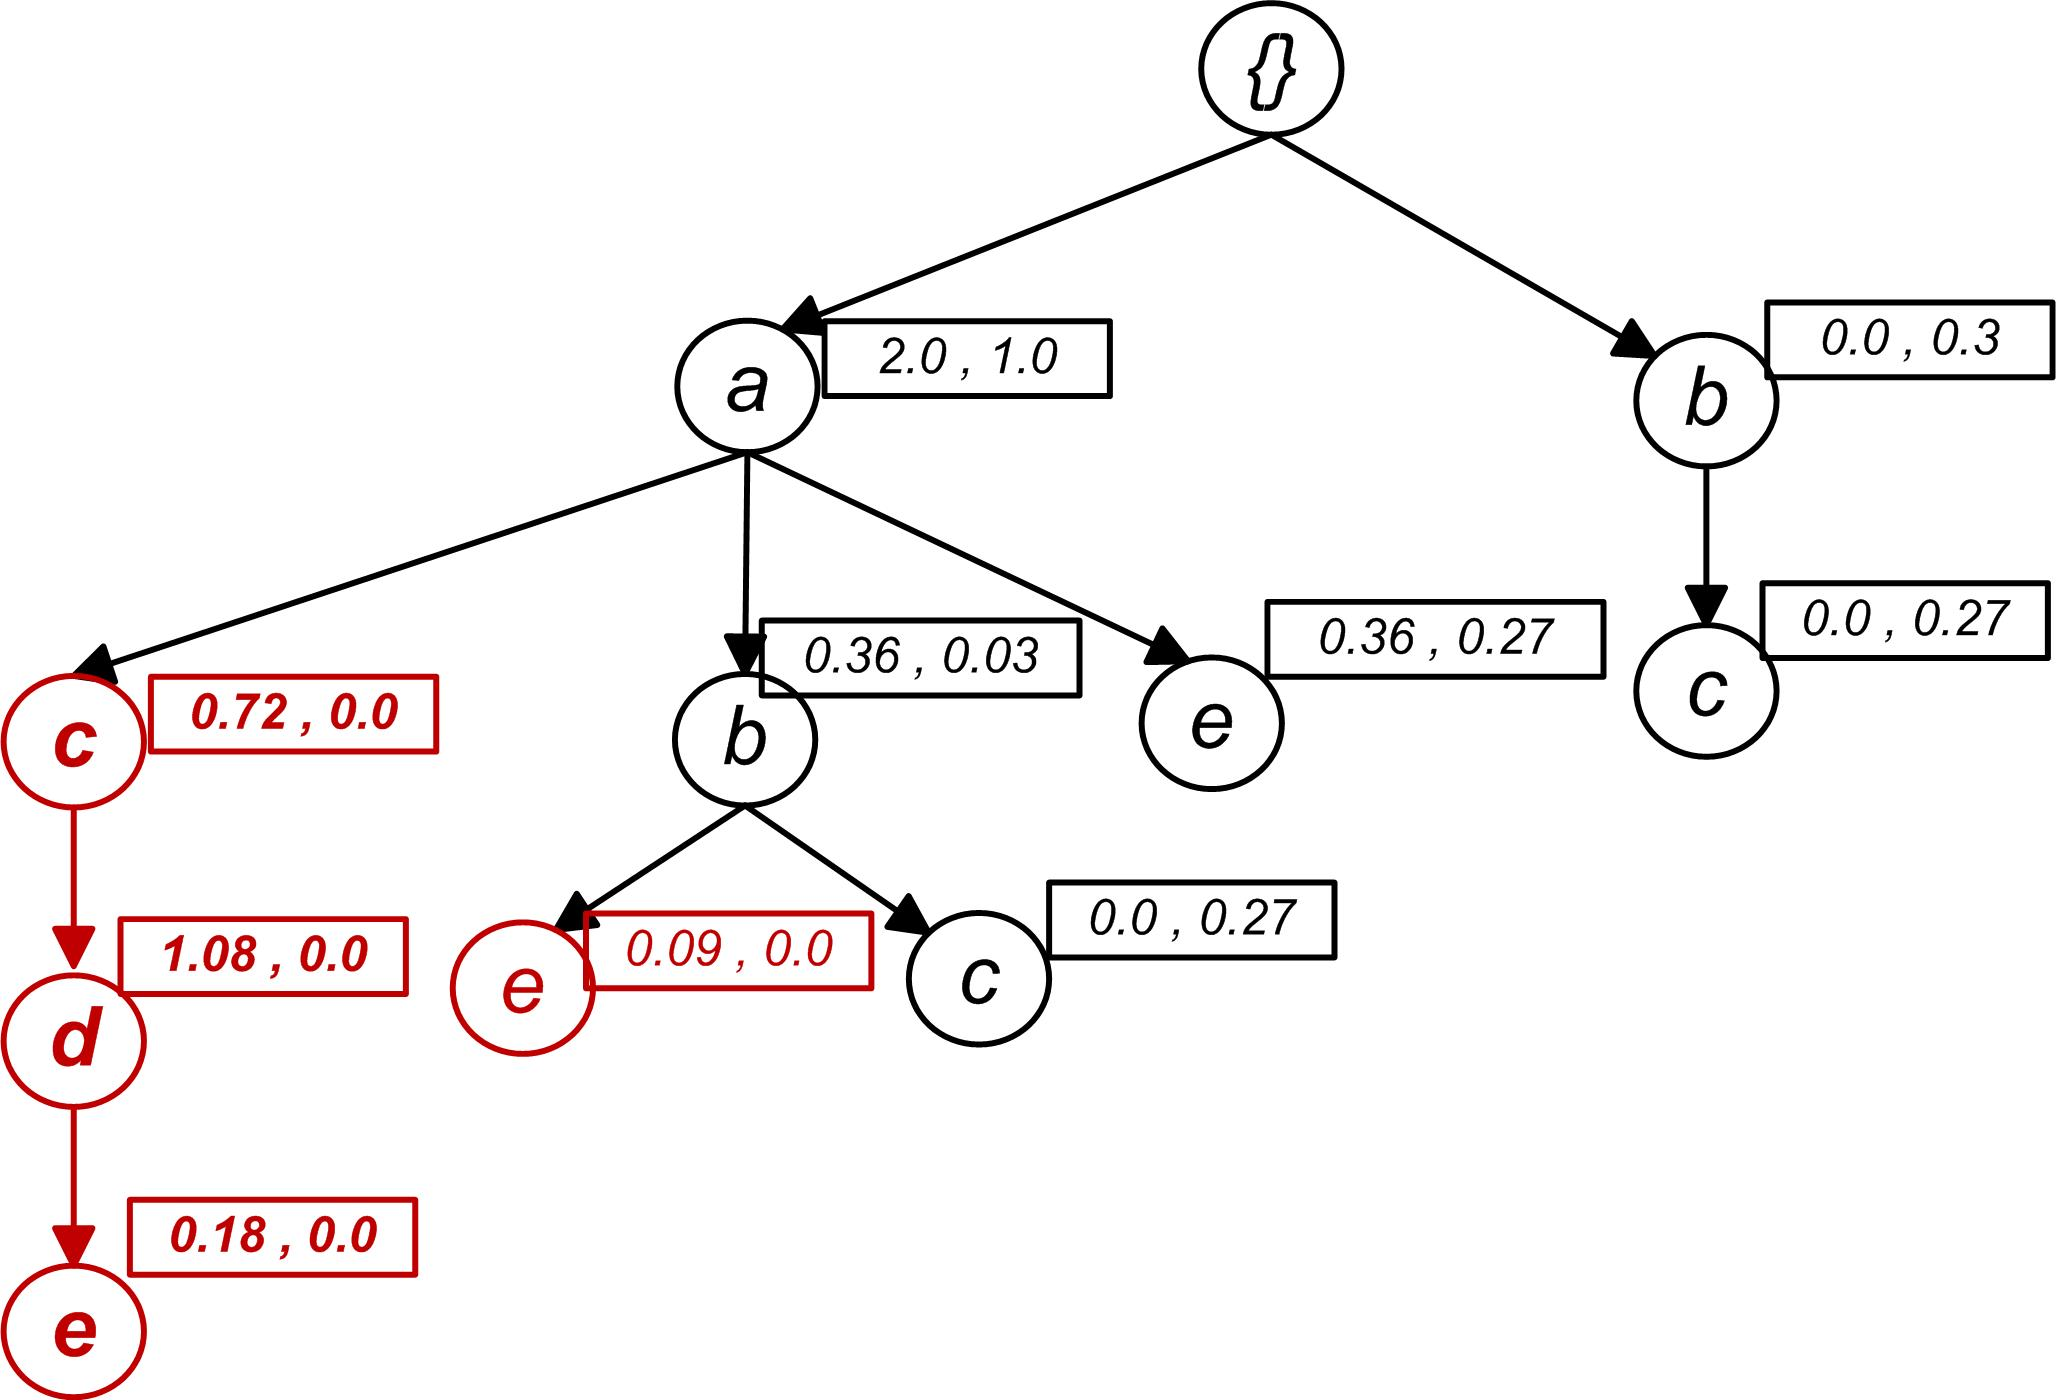
\includegraphics[width=\textwidth]{images/sim_06_slide.jpg}
\end{minipage}
\hfill
\begin{minipage}{0.20\textwidth}
  \centering
  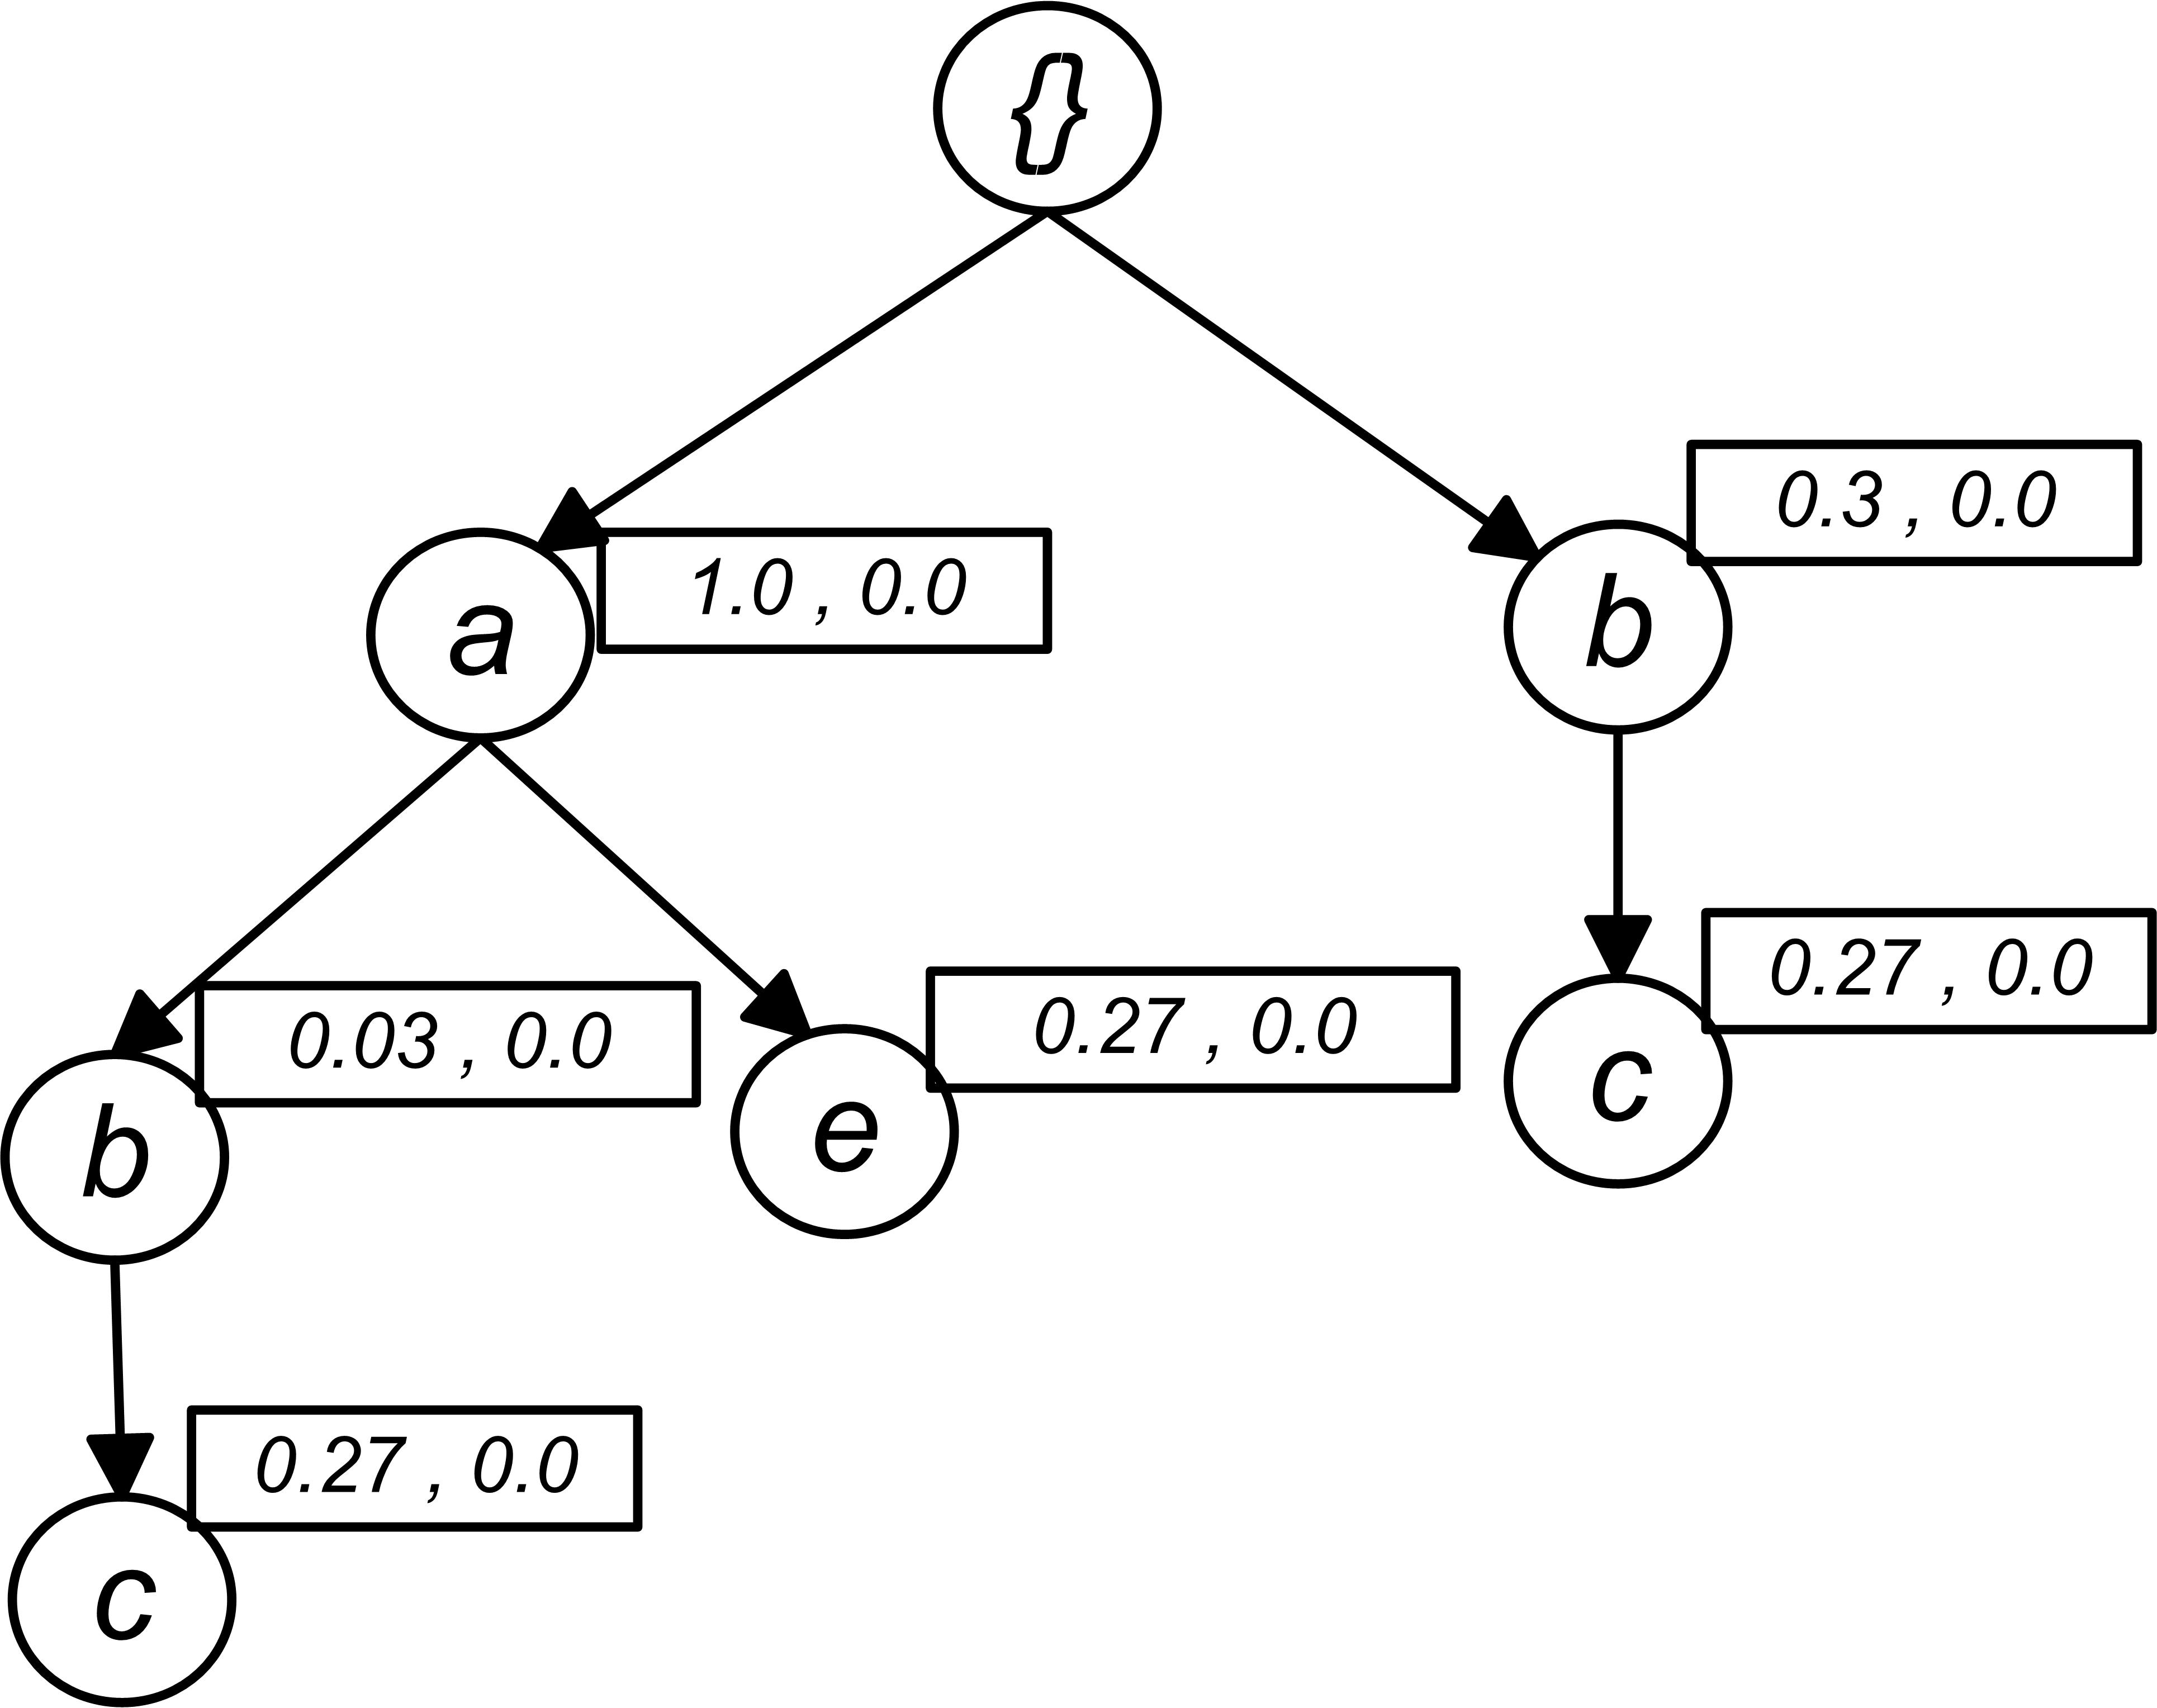
\includegraphics[width=\textwidth]{images/sim_06_slide_2.jpg}
\end{minipage}
\caption{Slide Window}
\label{figure:slide}
\end{figure}
    Now our window is completed and can our \emph{USFP-growth} mine \emph {US-tree}. When new transaction batch comes like \emph{Batch-3 (T\textsubscript{7}, T\textsubscript{8}, T\textsubscript{9})} comes to be inserted into the tree then first we have to slide the window. For this when we construct the tree we maintain a header table which contains the information for the oldest data. Thus pointer points to the oldest data can be found easily and slide the whole tree. Figure-\ref{figure:slide} shows the sliding and getting the old data removed tree and ready to insert next batch \emph{Batch-3}. After inserting \emph{Batch-3} we get the tree like Figure-\ref{figure:w2}. 
    %\documentclass{article}
%\usepackage{graphicx}
%\usepackage{caption}
%\usepackage{subcaption}
%
%\begin{document}
\begin{figure}
  \centering
	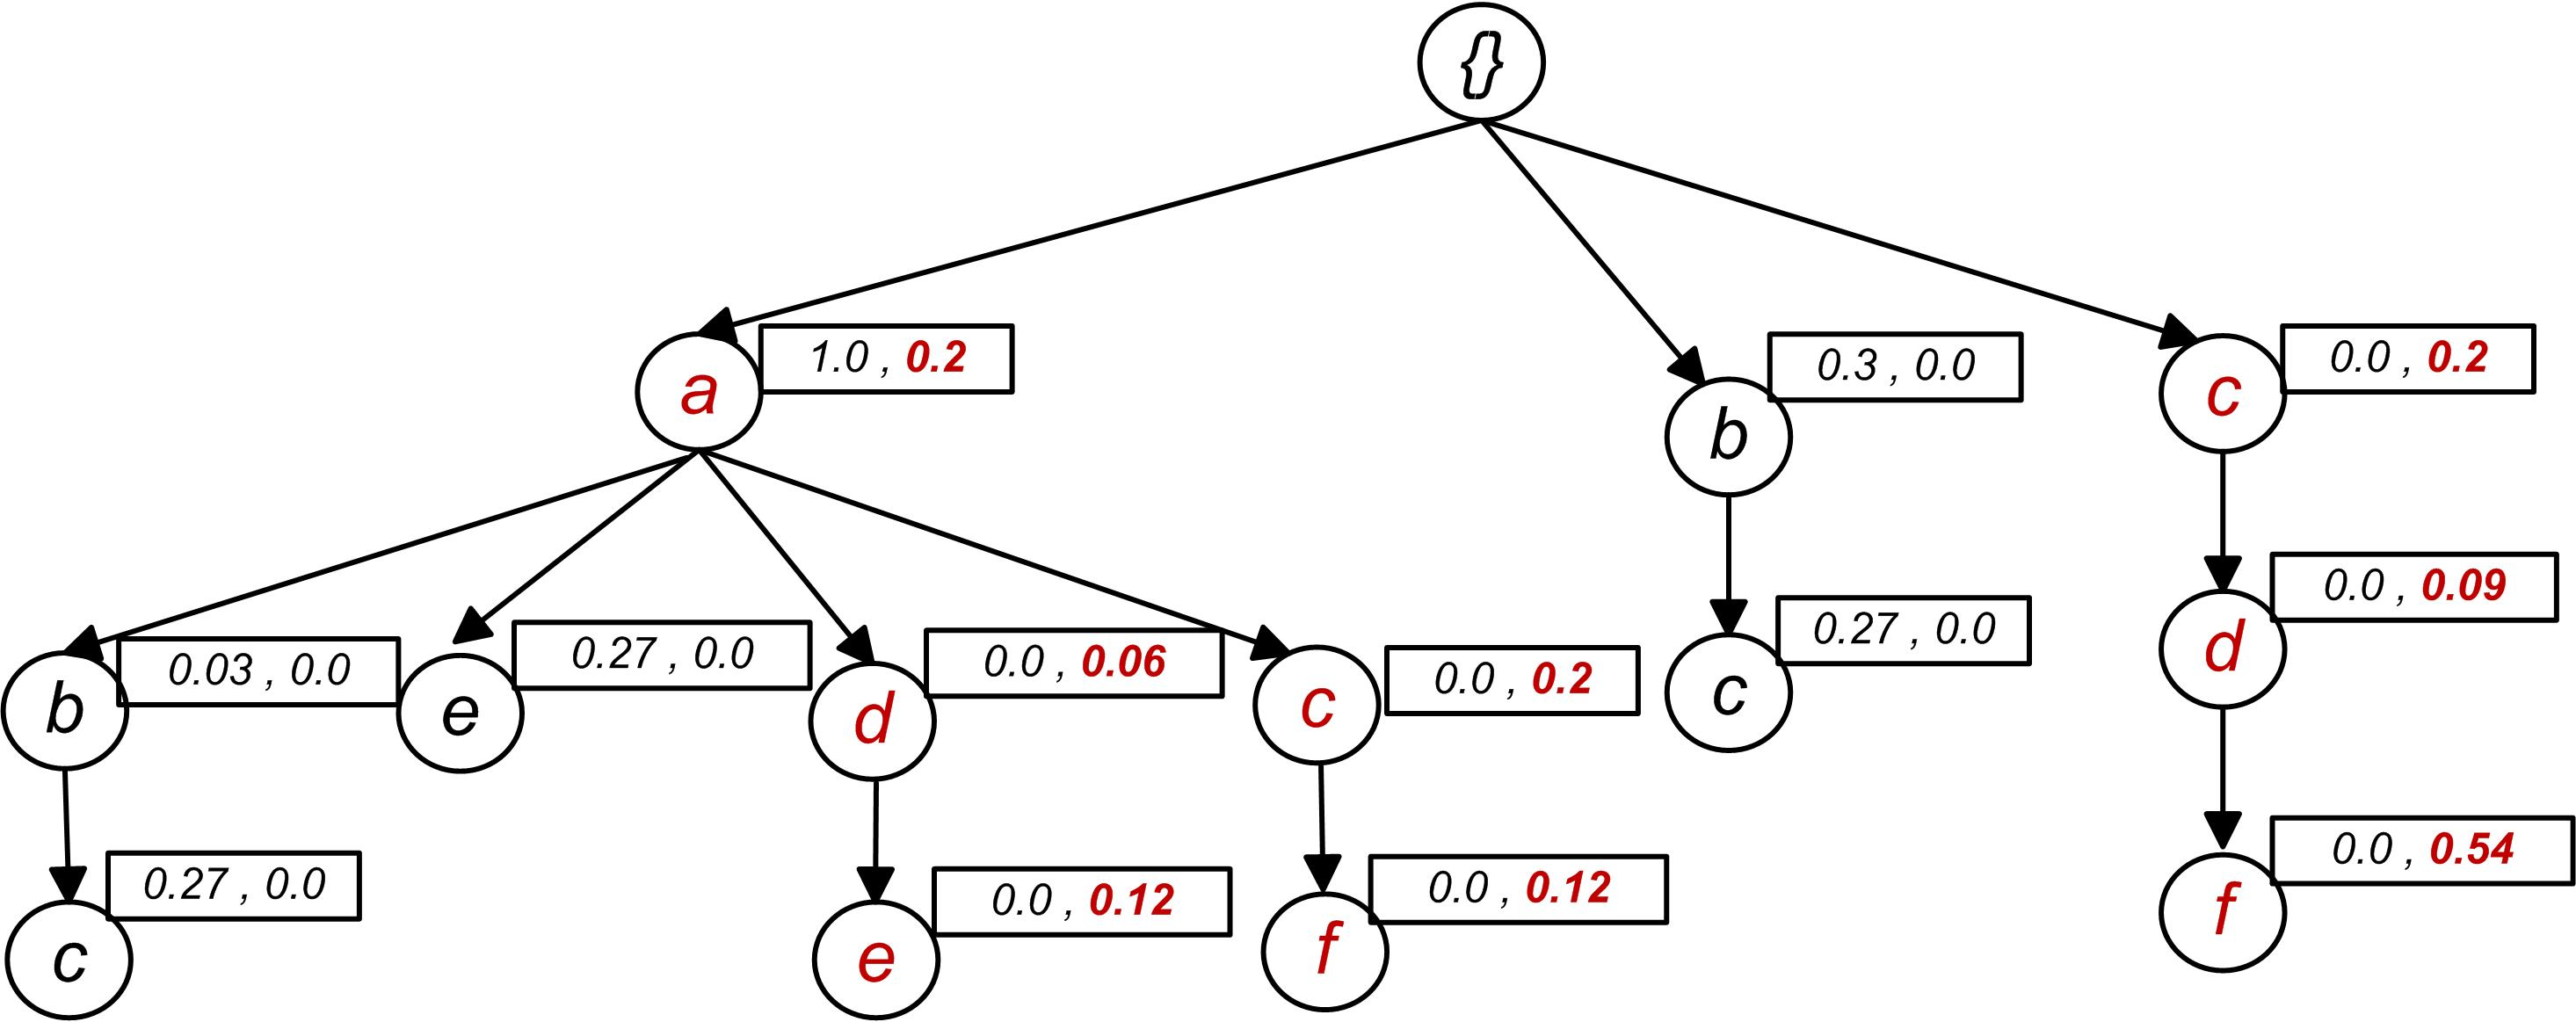
\includegraphics[width=.4\textwidth]{images/sim_789.jpg}  
	\caption{Inserting $T_7$, $T_8$, $T_9$ into US-tree after Sliding}
	\label{figure:w2}
\end{figure}
%\end{document}
    In the described \emph{US-tree} construction process we see that tree sharing is very much common and regular. That makes our tree very compact and memory needed to hold items becomes less. Moreover, the tree construction time improves surprisingly. When to mine this \emph{US-tree} we can gain a lot time when mining. As the tree size is small, conditional tree will be much more less when mining. We will gain a lot time when trying to mine the conditional trees. In the experimental result section we will provide necessary graphs for our simulations.
\subsubsection{FPUS-growth Mining Approach}
In this section we will discuss about our mining approach \emph{USFP-growth} That will find frequent patterns. For mining we used \emph{FP-growth} like approach. Generally, we can remove all the nodes having support less than \emph{minimum support}. From header table we get such information that which nodes is less than \emph{minimum support}. We told earlier that for \emph{U\textsuperscript{cap}} value we took the upper limit, we also can we can remove all the nodes having prefix value less than \emph{minimum support}. In this process we can eliminate most of the infrequent nodes from tree. For this purpose we used header table that was created when creating the \emph{US-tree}. Then we construct conditional tree starting from the lowest support holding node. From header table we also get the position of all nodes containing same item in the tree.

Let’s mine the tree we constructed earlier. Figure-\ref{figure:min_before} is \emph{US-Tree} for mining and corresponding header table before starting mining. From the header table, we get that support of \emph{a} is $3.00$, \emph{b} is $1.00$, \emph{c} is $3.30$, \emph{d} is $1.20$, \emph{e} is $0.60$. So, \emph{e} is not frequent for one item set frequent pattern. So it is sure that no item set contains \emph{e} will be frequent. That is the basic upward closure property of frequent item set. So we remove all the nodes of \emph{e} and get the new mining tree Figure-\ref{figure:min_ready} and its header table. Here we find all one item sets that are frequent and that is \emph{\{a\}, \{b\}, \{c\} \{d\}} Now we will construct conditional tree for the found frequent one item and mine the conditional tree. But items having total \emph{U\textsuperscript{cap}} less than \emph{minimum support} is not needed to construct conditional tree because this \emph{U\textsuperscript{cap}} value has been take as the upper bound. So total \emph{U\textsuperscript{cap}} value less than \emph{minimum support} indicates that item must not be exists in the $2$ or more frequent item set. So we do not construct conditional tree for these items.

We construct conditional tree from items having lowest total \emph{U\textsuperscript{cap}} value greater than \emph{minimum support}. As \emph{b} having total \emph{U\textsuperscript{cap}} is $.69$ \emph{b}, is ignored for constructing conditional tree. Then the next candidate is \emph{d}. From header table pointer we find that there is only one path item \emph{d} exists in the mining tree Figure-\ref{figure:min_ready}. That is \{\emph{a, c, d}\}:$1.08$. So we create conditional tree and update all nodes mining probability with \emph{d's} \emph{U\textsuperscript{cap}} $1.08$. For this conditional tree Figure-\ref{figure:d_cond} the header tables says all the nodes in the tree are having \emph{U\textsuperscript{cap}} greater than \emph{minimum support} $.9$. So, all the items are ready to be constructed as conditional tree. As here is only one branch so we do not further construct conditional tree and take all the combinations as frequent items Figure-\ref{figure:d_cond} Table. So we find \emph{\{dc\}, \{da\}, \{dca\}} as frequent pattern. Next we create conditional tree for \emph{c}. Here c exists in the tree for three path those are \emph{\{a, c\} : $0.72$ , \{a , b, c\} : $.027$ and \{b, c\} : $0.27$}. So we create conditional tree (Figure-\ref{figure:c_cond}). Total mining value of \emph{c} is the sum of item caps in each respective path of \emph{c}. From the header we see that \emph{b} has total cap having less than \emph{minimum support} so we remove \emph{b} and create two item set \emph{\{ca\}}. Next we construct \emph{ca} conditional tree that contains only root (\emph{\{\}}). So no further tree is needed to be constructed and minned. Than we create conditional tree for \emph{a}. And find only root \emph{\{\}}. Thus we get all the frequent patterns. All the patterns are \emph{\{a\}, \{b\}, \{c\} \{d\}, \{dc\}, \{da\}, \{dca\} and \{ca\}}. As we have found all patterns from upper bound, so that it is guaranteed that there will be no false negative. But some false positive can be exists in the found frequent item set as there may be some value less than max value we assumed. So in the next section we will show an approach that eliminates the all false positives (if exists) in the data set.
    %\documentclass{article}
%\usepackage{caption}
%\usepackage{graphicx}
%\begin{document}

\begin{figure}
\begin{minipage}{0.20\textwidth}
  \centering
  
	\begin{center}
	\begin{tabular}{ |c|c|c| } 
 	\hline
 		Item&\emph{U\textsuperscript{cap}}&Support\\ \hline\hline
 		a &  3.00  & 3.00	\\ \hline
 		c &  1.26  & 3.30	\\ \hline
 		d &  1.08  & 1.20	\\ \hline
 		e &  0.54  & 0.60	\\ \hline
 		b &  0.69  & 1.00	\\ \hline
\end{tabular}
\end{center}   
  \captionof{table}{Header Table of US-tree}
\end{minipage}
\hfill
\begin{minipage}{0.20\textwidth}
  \centering
  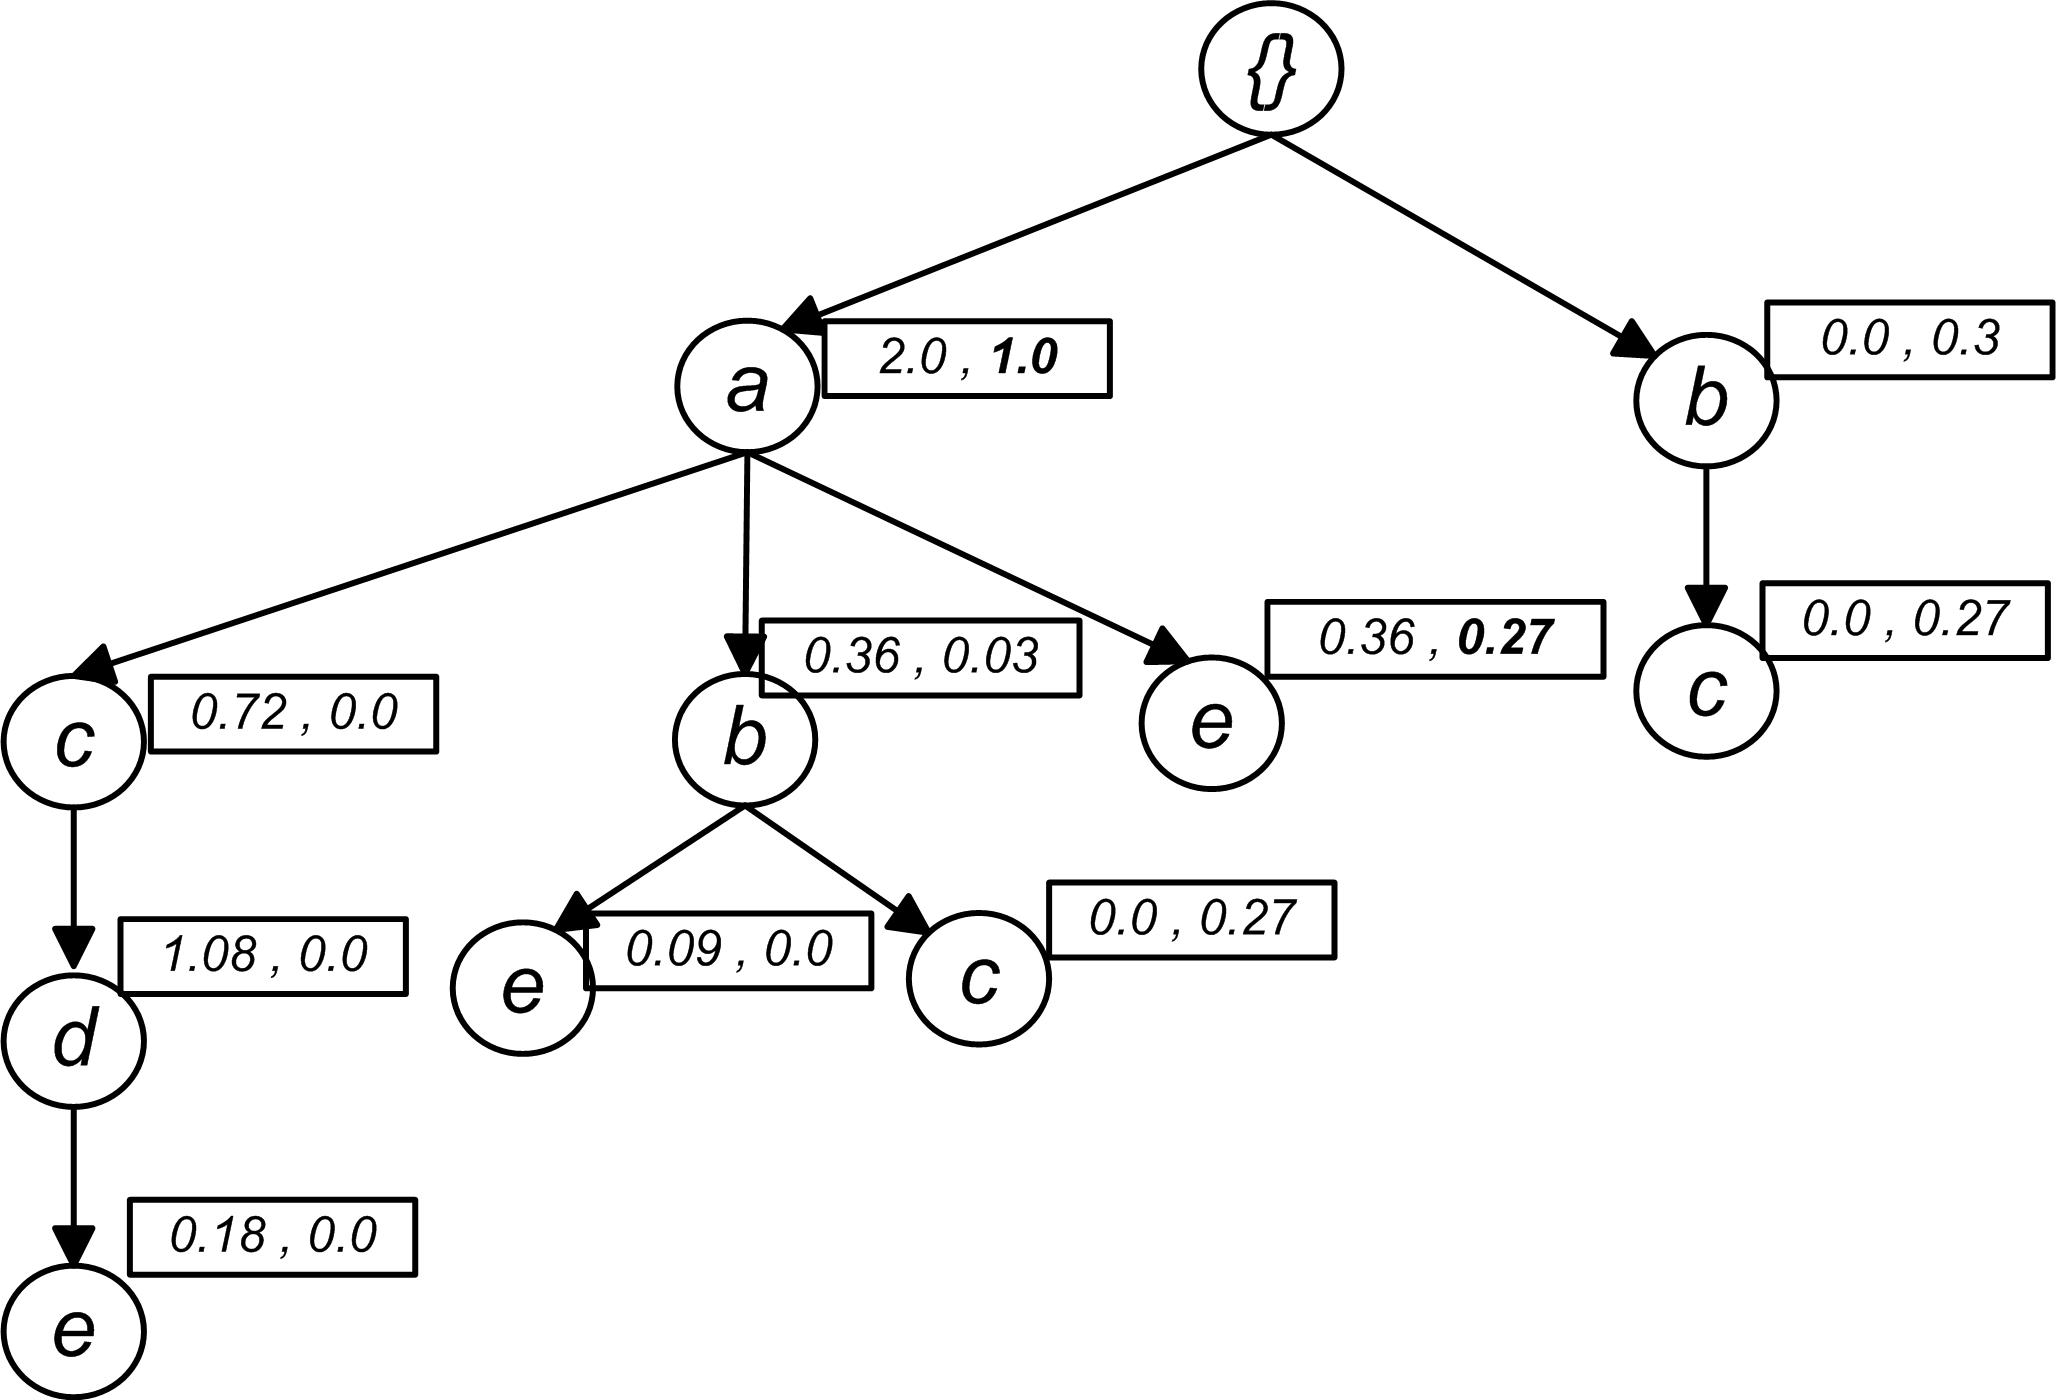
\includegraphics[width=\textwidth]{images/us_tree.jpg}
  \captionof{figure}{US-tree}
\end{minipage}
\caption{US-tree and Header Table}
\label{figure:min_before}
\end{figure}


\begin{figure}
\begin{minipage}{0.20\textwidth}
  \centering
  
	\begin{center}
	\begin{tabular}{ |c|c|c| } 
 	\hline
 		Item&\emph{U\textsuperscript{cap}}&Support\\ \hline\hline
 		a &  3.00  & 3.00\\ \hline
 		c &  1.26  & 3.30\\ \hline
 		d &  1.08  & 1.20\\ \hline
 		b &  0.69  & 1.00\\ \hline
\end{tabular}
\end{center}  
  
  
  \captionof{table}{Header Table for Mining}
\end{minipage}
\hfill
\begin{minipage}{0.20\textwidth}
  \centering
  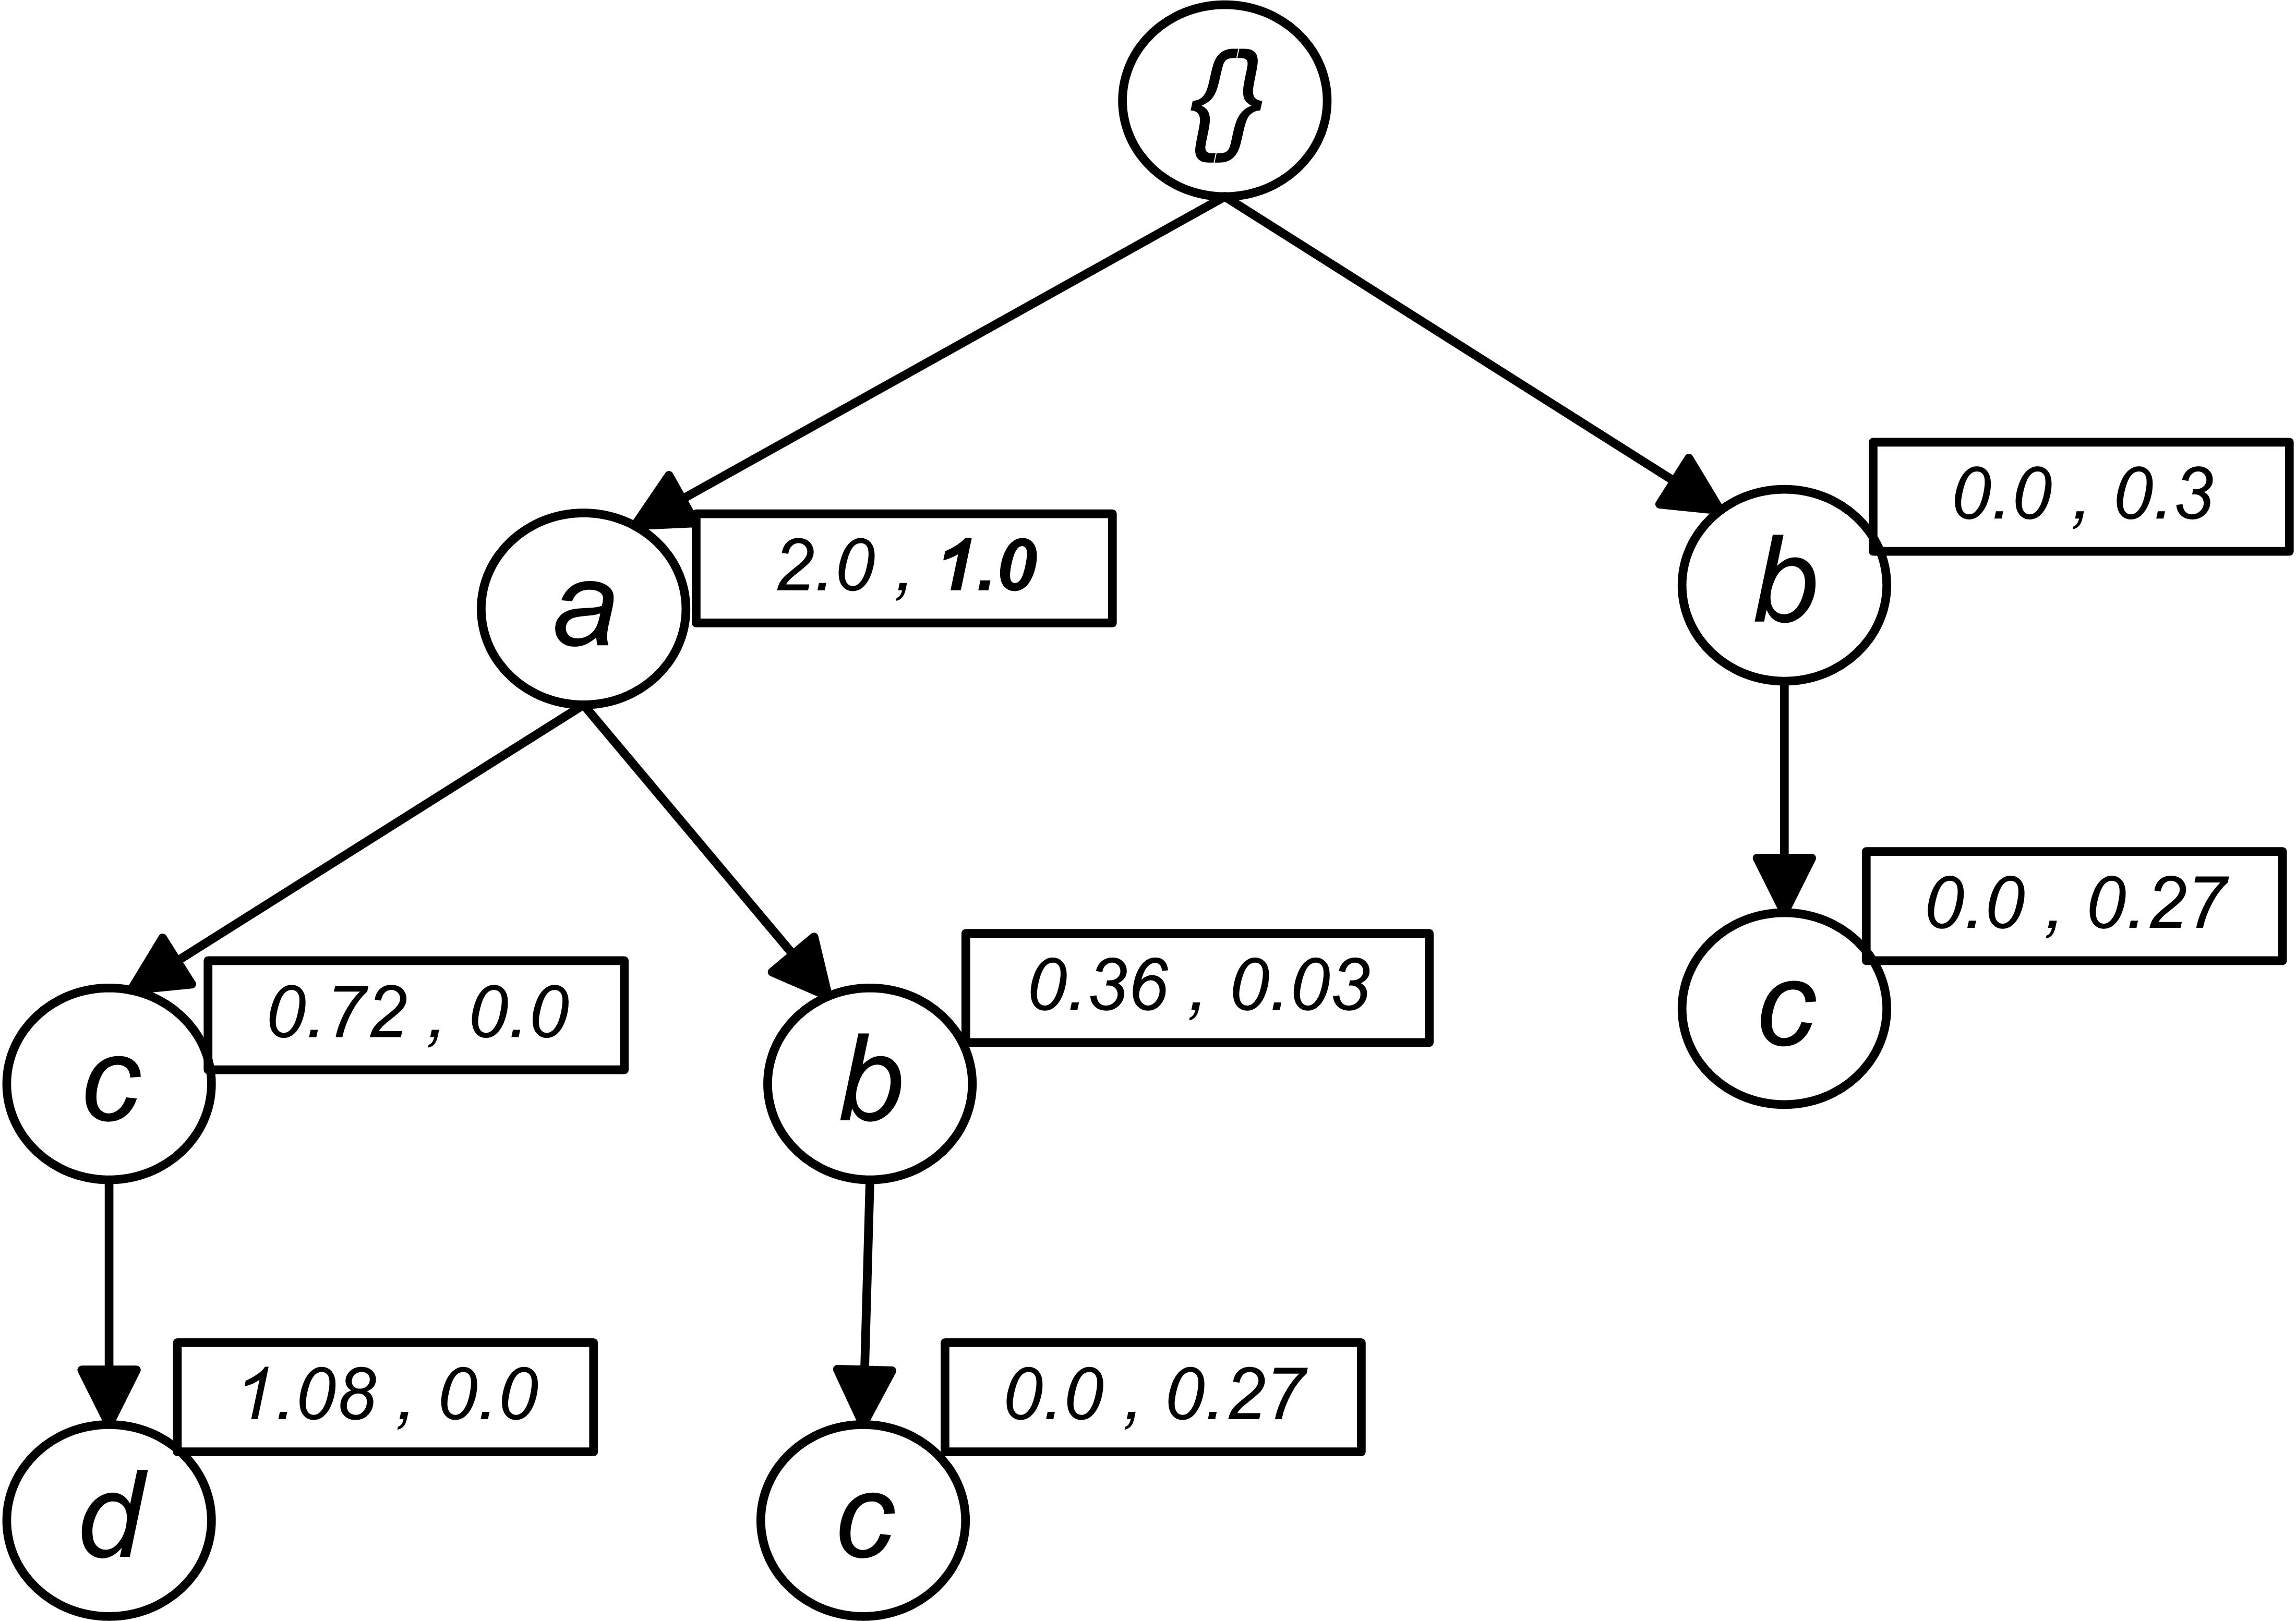
\includegraphics[width=\textwidth]{images/M_TREE.jpg}
  \captionof{figure}{US-tree for Mining}
\end{minipage}
\caption{US-tree and Header Table for Mining}
\label{figure:min_ready}
\end{figure}
%\end{document}
    %\documentclass{article}
%\usepackage{caption}
%\usepackage{graphicx}
%\begin{document}
\begin{figure}
\begin{minipage}{0.20\textwidth}
  \centering
	\begin{center}
	\begin{tabular}{ |c|c| } 
 	\hline
 		Item&Value\\ \hline\hline
 		a &  1.08  	\\ \hline
 		c &  1.08   	\\ \hline
 		
\end{tabular}
\end{center}  
  \captionof{table}{d-cond Tree Header }
\end{minipage}
  \hfill
\hfill
\begin{minipage}{0.10\textwidth}
  \centering
  \hfill
  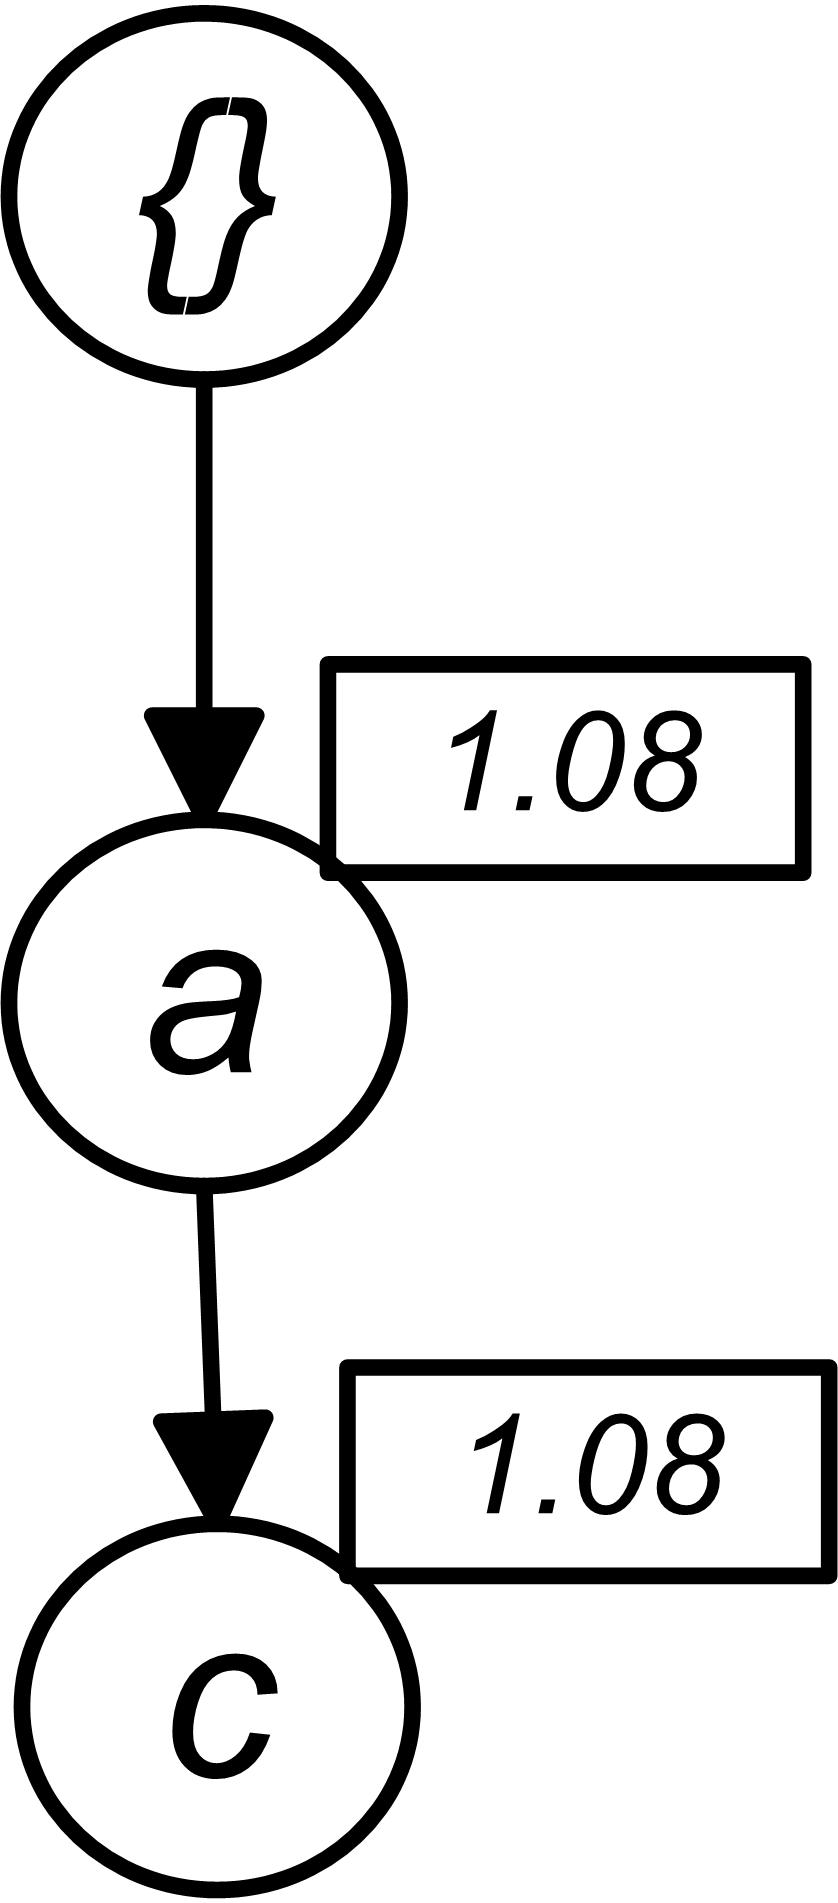
\includegraphics[width=.65\textwidth, height=2.5cm]{images/D_COND.jpg}
  \hfill
\end{minipage}
\hfill
\begin{minipage}{0.15\textwidth}
  \centering
  
	\begin{center}
	\begin{tabular}{ |c| } 
 	\hline
 		FPs \\ \hline\hline
 		dc  	\\ \hline
 		da   	\\ \hline
 		dca   	\\ \hline
 		
\end{tabular}
\end{center}  
  \captionof{table}{FPs for $d$-cond Tree }
\end{minipage}
\caption{$d$-cond Tree and Corresponding Header}
\label{figure:d_cond}
\end{figure}
\begin{figure}
\begin{minipage}{0.15\textwidth}
  \centering
	\begin{center}
	\begin{tabular}{ |c|c| } 
 	\hline
 		Item&Value\\ \hline\hline
 		a &  .99  	\\ \hline
 		b &  .54   	\\ \hline
\end{tabular}
\end{center}  
  \captionof{table}{$c$-cond Tree Header }
\end{minipage}
  \hfill
\begin{minipage}{0.14\textwidth}
  \centering
  \hfill
  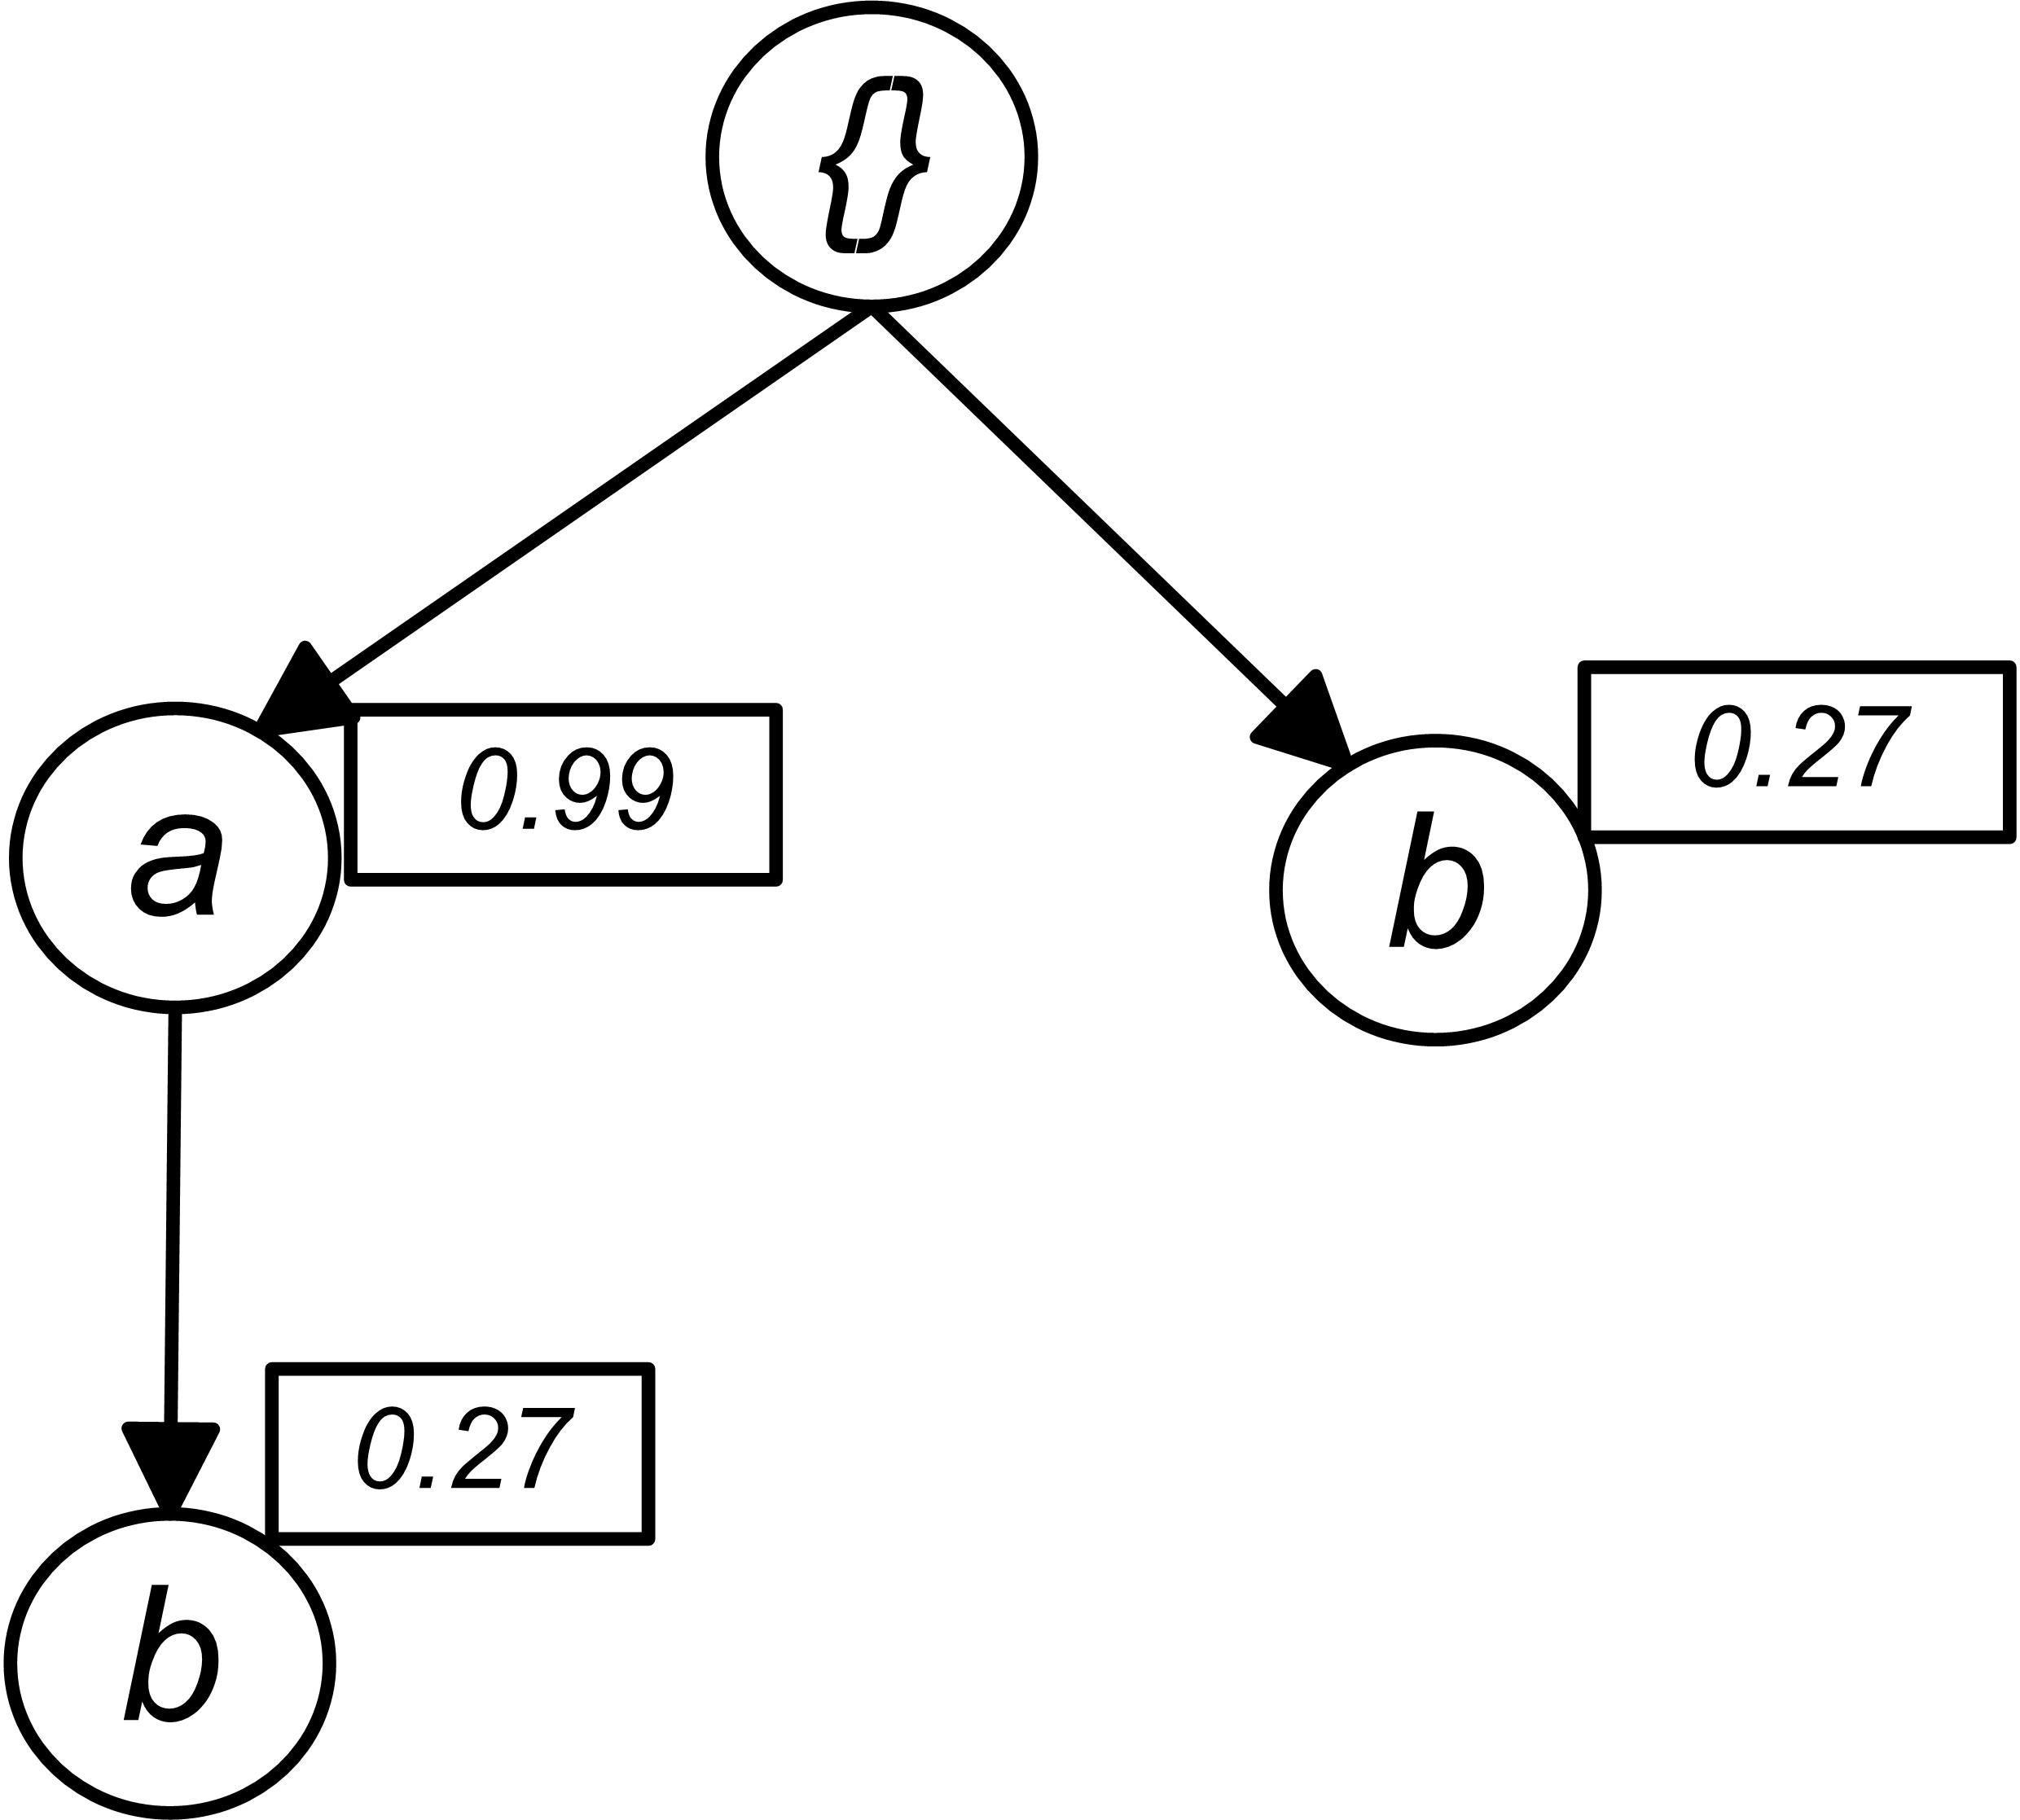
\includegraphics[width=.8\textwidth, height=2.5cm]{images/C_COND.jpg}
  \hfill  
\end{minipage}
\hfill
\begin{minipage}{0.15\textwidth}
  \centering  
	\begin{center}
	\begin{tabular}{ |c| } 
 	\hline
 		FPs \\ \hline\hline
 		ca  	\\ \hline
 		
\end{tabular}
\end{center}   
  \captionof{table}{FPs for $c$-cond Tree}
\end{minipage}
\caption{$c$-cond Tree and Corresponding Header}
\label{figure:c_cond}
\end{figure}







\begin{figure}
\centering
  
\includegraphics[width=.05\textwidth]{images/A_COND.jpg}
\caption{$a$-cond Tree}
\label{figure:a_cond}
\end{figure}

%\end{document}

\subsubsection{False positive reduction}
    False positives are such patterns those are exist in the frequent pattern list but not actually frequent. False negatives are such patterns those does not exist in the frequent pattern list but actually frequent. As our whole process of \emph{U\textsuperscript{cap}} assignment, construction of \emph{US-tree} and \emph{USFP-growth} mining algorithm, all are process are based on taking upper value of two item set supports, our process may create some false positives but no false negatives. In this section we will discuss about finding and eliminating all the false positives from found patterns from \emph{USFP-growth} mining result. For this elimination process we just use two scans of transactions. In the first scan we eliminate the infrequent one item set. In the second scan we update \emph{frequent tree} exact support that makes easily to find infrequent items if exists in our frequent item found. The process is given below.

In the previous sections we described about tree construction and mining approach. Mining transaction table-\ref{table:transaction_batch} we found \emph{\{a\}, \{b\}, \{c\} \{d\}, \{dc\}, \{da\}, \{dca\}} and \emph{\{ca\}} as frequent patterns. From the patterns we first construct a pattern tree from the patterns. This tree is very much easier to construct. For tree construction we first create root node \emph{\{\}}. Then take each frequent item and insert into the root node as a child. for \emph{a}, \emph{b}, \emph{c}, \emph{d} we just insert as child as it does not exists in the tree. For \emph{dc} do not create new node for \emph{d} but create a new node \emph{c} as child of \emph{d} as there is no \emph{c} exists in the child of \emph{d}. Thus we construct the whole frequent pattern tree for further identification of infrequent patterns.

Next, in the first scan of inserted transactions, we remove one item infrequent all items from transactions. Figure-\ref{figure:frequent_patterns_final} table shows the transaction table after eliminating all nodes accepts one item frequent. As for one item frequent checking we did not take any upper bound limit we get exact one item frequent patterns. From our \emph{Frequent Item Tree} all the children of \emph{root \{\}} are frequent and there is no false positive. So we can get \emph{\{a\}, \{b\}, \{c\} \{d\}} one item frequent set and without these all other items are infrequent.  Then in the second scan we take each transaction and update each nodes support. In the tree we update value with the equation-\ref{equation:exp_sup}. After scanning second time our \emph{Frequent Item Tree} becomes full fill with all information to find infrequent exists in our patterns. For this we need to traverse the \emph{Frequent Item Tree}. As the tree contains all nodes with its own support we get the true infrequent. For example, for \emph{\{d, a\}} path \emph{a : 0.89} as the actual support for {da : 0.89} pattern. We find this in frequent, so we can easily eliminate. Figure-\ref{figure:frequent_patterns_final} shows the identifying all the frequent item set infrequent. So we can eliminate all the false positives.    And find the exact frequent patterns. From the tree we find the patterns \emph{\{a\}, \{b\}, \{c\} \{d\} and \{dc\}}.
      \begin{figure}[]
        \centering
            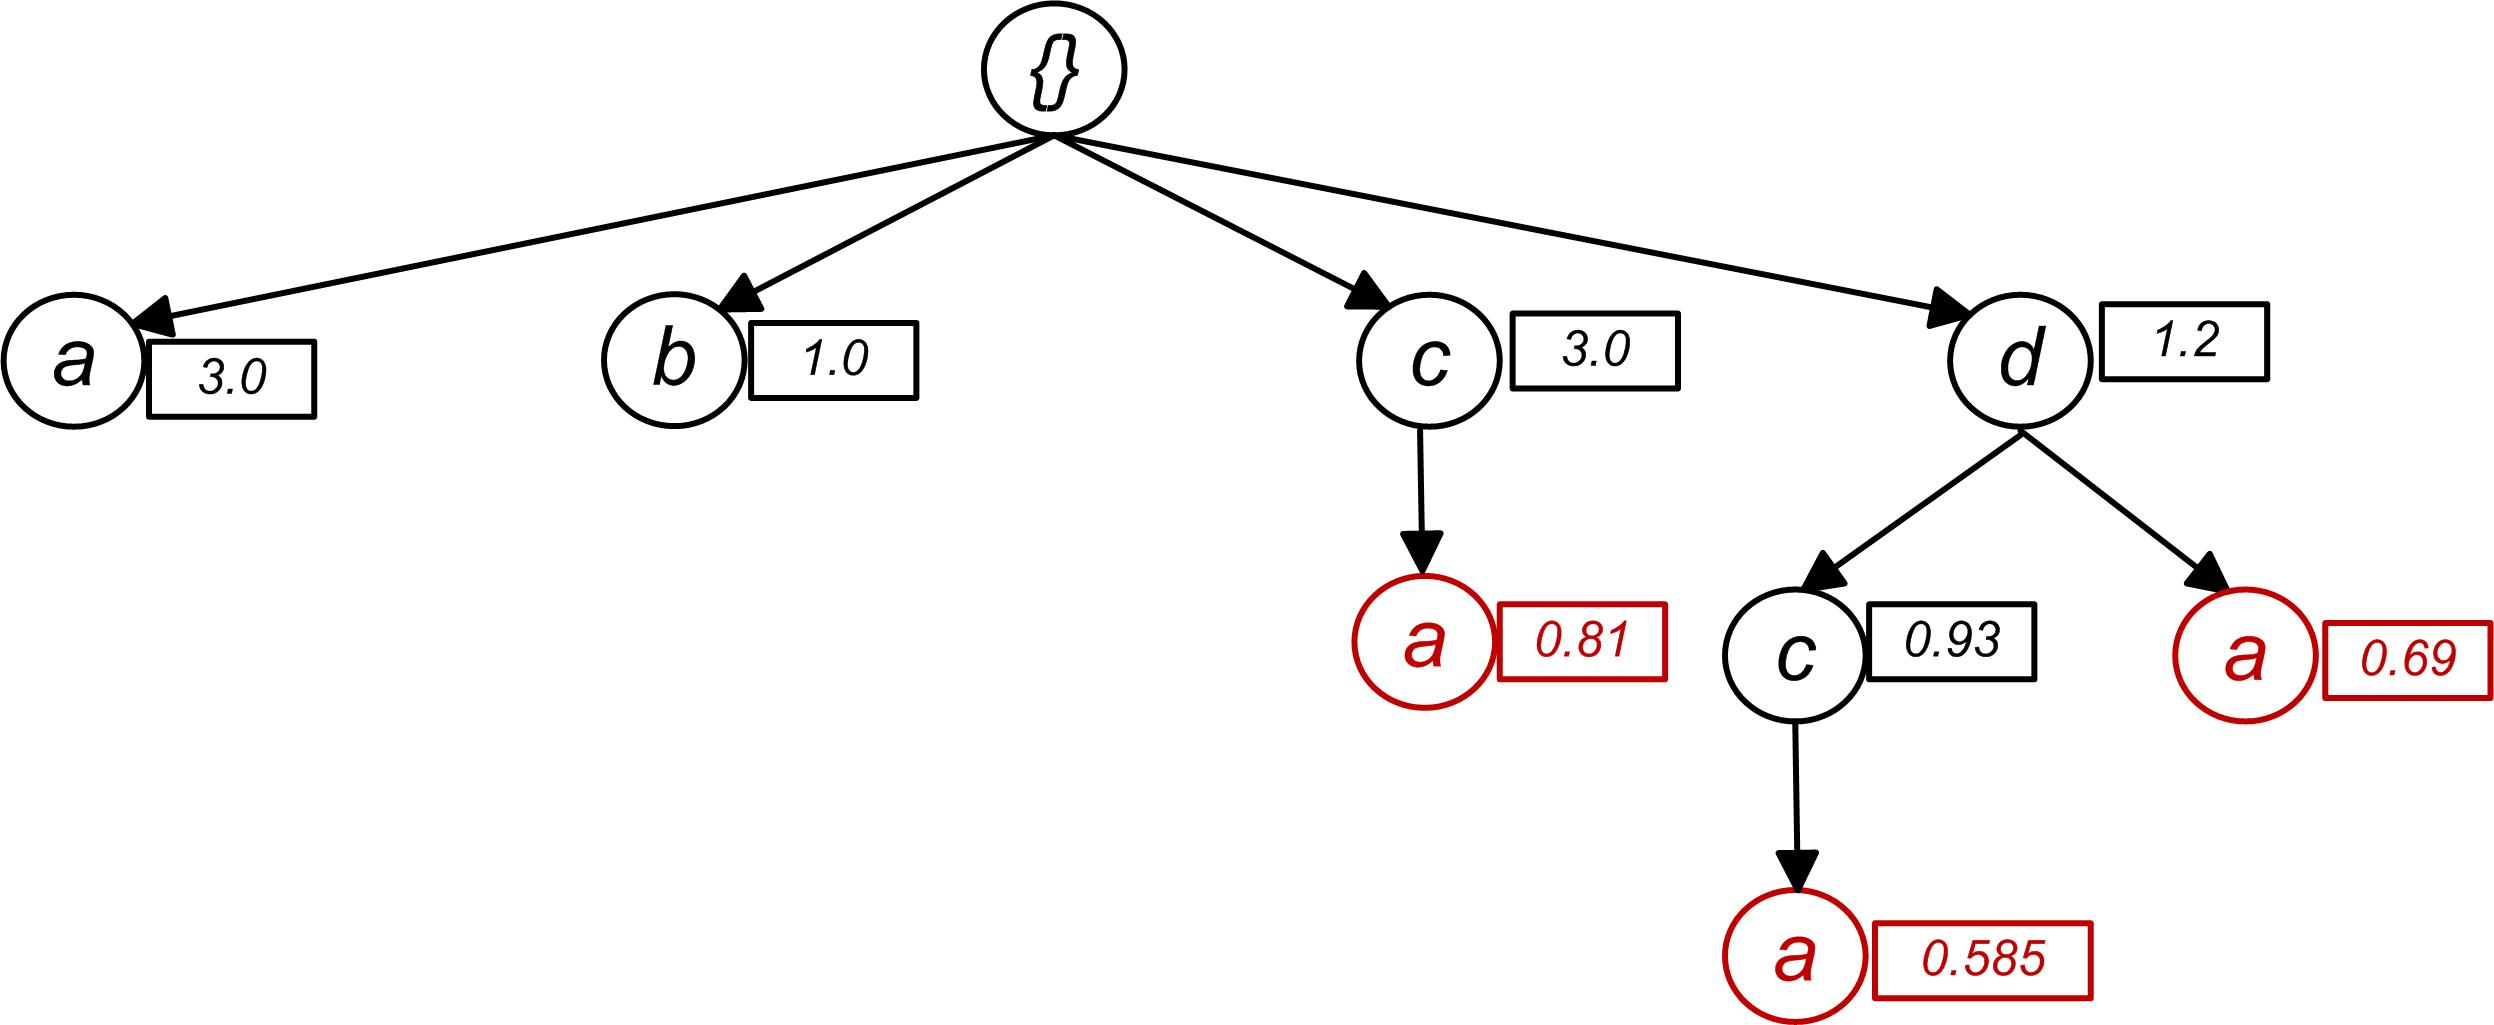
\includegraphics[width=.45\textwidth]{images/frequent_tree_final}
        \caption{Pattern Tree Identifying False Positives}
        \label{figure:frequent_patterns_final}
  \end{figure}



\begin{figure}
\begin{minipage}{0.15\textwidth}
  \centering
  
	\begin{center}
	\begin{tabular}{ |c| } 
 	\hline
 		FPs\\ \hline\hline
 		a \\ \hline
 		b \\ \hline
 		c \\ \hline
 		d \\ \hline
 		dc \\ \hline
 		da \\ \hline
 		dca \\ \hline
 		ca \\ \hline
\end{tabular}
\end{center}  


  \captionof{table}{Frequent Patterns}
\end{minipage}
\hfill
\begin{minipage}{0.30\textwidth}
  \centering
  
  \begin{center}
  \begin{tabular}{ |c|c| } 
  \hline
    No & Items \\ \hline\hline
    T\textsubscript{1} & \emph{a(0.9),c(0.6),d(0.5)}\\ \hline
    T\textsubscript{2}& \emph{a(0.9),b(0.4),e(0.1)}\\ \hline
    T\textsubscript{3}& \emph{a(0.2),c(0.9),d(0.7)}\\ \hline
    T\textsubscript{4}& \emph{b(0.3),c(0.9)}\\ \hline
    T\textsubscript{5}& \emph{a(0.1),b(0.3),c(0.9)} \\ \hline
    T\textsubscript{6} & \emph{a(0.9),e(0.3)
}\\ \hline
\end{tabular}
\end{center}  
  \captionof{table}{Transaction Table after Removing Infrequent}


\end{minipage}
\label{figure:frequent_patterns}
\end{figure}







\section{Experimental Results}







We have performed a number of simulations in our experiment on both synthetic database and real-world database. The data are taken from dataset repository ~\cite{dataset}. Our experiment shows that \emph{US-tree} (Uncertain Stream tree) is very much compact. This tree construction technique can make the items share one single node. This compactness of \emph{US-tree} surprisingly helps the mining, \emph{USFP-growth} (Uncertain Stream Frequent Pattern growth) process to gain a lot in run-time and memory. Pattern tree can be used to find max pattern and closed pattern. Performance tests from our experiment show that \emph{US-tree} tree construction technique and \emph{USFP-growth} mining algorithm can run on any uncertain stream database with any support threshold, window size, and batch size. Our experimental result shows that these techniques are much faster and scalable frequent pattern mining technique. As we have proposed a new approach for finding frequent patterns over uncertain data we have compared performance with itself for comparing correctness of our approach. Then we have compared with \emph{SUF-growth}. We have tried to compare in all aspects to prove our approach's correctness, run-time efficiency, and memory efficiency. We have collected the real-life and synthetic datasets from the frequent item-set mining repository ~\cite{dataset}, those were collected for certain databases. Then we have used our own probabilistic tool and technique to generate the existential probability of each item of the each transaction of the database. Real life data set actually follows gaussian distribution that is normal distribution. It actually says that in real world extreme cases are minimum and average cases are maximum. We have used \emph{Java pseudo random} generate the existential probability for each item of all the transaction of the database with gaussian distribution. By assigning these probability value to each item, we have generated the uncertain database for both real life database and synthetic database found from dataset repository ~\cite{dataset}. However, one can give existential probability by any distribution according to need. We have set several properties for this evaluation from experimental result. Batch size vs running time, window size vs running time, transactions in a window vs false positive count for correctness; tree construction time per window and total database vs minimum support, mining time per window and total database vs minimum support, total time to complete per window and total database vs minimum support, total tree node in tree per window vs minimum support, total memory needed by mining process vs minimum support for comparison with existing approaches.

In this section, we have provided experiment analysis. In the experiment, we have focused on (1) correctness of our proposed algorithm and (2) the comparison with existing algorithm SUF-growth ~\cite{suf_growth}. For the extensive experiment, we have chosen the mushroom dataset  and T40I10D100K database. The reason we have chosen these two datasets is, the mushroom  is real life dataset and dense dataset whereas T40I10D100K  is synthetic and sparse dataset generated by a generator from the IBM Almaden Quest. Table \ref{table:dataset} shows the details the properties for dataset . Later we have also taken chess  for comparison with the algorithm. The experimental results have been given in the following subsections.
\subsection{Algorithm Performance Analysis}

\paragraph{Total Database Size Change Effect}Our experiment shows clearly that our proposed tree construction algorithm \emph{US-tree}, tree mining algorithm \emph{USFP-growth} works nicely with any size of window, batch or transaction size. For the different size of the database (transaction count in a tree), this algorithm works extensively. Figure-\ref{result:g_m_const_tran} shows the total runtime (includes tree construction, mining, and false positive reduction) change with the growth of the size of the mushroom dataset. Figure-\ref{result:g_t10_const_tran} the same characteristic for T40I10D100K dataset. Figure-\ref{result:g_m_const_tran_mem} and figure-\ref{result:g_t10_const_tran_mem} shows the total nodes change in a tree while the size of database grows for databases corresponding to mushroom and T40I10D100K database. The growth of the graphs is very much regular. From these graphs, it is clearly visible that, with the growth of total transaction the time increases and this certainly proves the scalability of our algorithm. 

        \begin{figure}[h]
        \centering
            %mark = star, diamond, square, otimes
%\documentclass{article}
%\usepackage{pgfplots}
%\usepackage[justification=centering]{caption}
%\pgfplotsset{compat=newest}
%\begin{document}
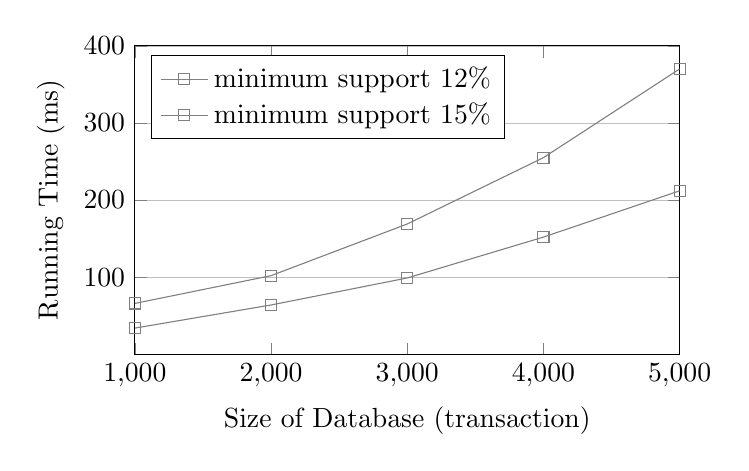
\begin{tikzpicture}
\begin{axis}[
	width=8.5cm,
	height=5.5cm,
    xlabel={Size of Database (transaction)},
    ylabel={Running Time (ms)},
    xmin=1000, xmax=5000,
    ymin=0, ymax=400,
    xtick={1000,2000,3000,4000,5000},
    ytick={100,200,300,400},
    legend pos=north west,
    ymajorgrids=true,
    grid style={line width=.2pt,draw=gray!50},
]
 
\addplot[
    solid,color=gray, every mark/.append style={solid, fill=gray}, mark=square
    ]
    coordinates {
		(1000,34)
		(2000,64)
		(3000,99)
		(4000,152)
		(5000,212)

	};
    \addlegendentry{minimum support 12\%}
	
\addplot[
    solid,color=gray, every mark/.append style={solid, fill=gray}, mark=square
    ]
    coordinates {
		(1000,66)
		(2000,102)
		(3000,169)
		(4000,255)
		(5000,370)

	};
    \addlegendentry{minimum support 15\%}

\end{axis}
\end{tikzpicture}
%\end{document}
        \caption{Size of Database vs Runtime for Mushroom ~\cite{dataset} Dataset }
        \label{result:g_m_const_tran}
        \end{figure}
        \begin{figure}[h]
        \centering
            %mark = star, diamond, square, otimes
%\documentclass{article}
%\usepackage{pgfplots}
%\usepackage[justification=centering]{caption}
%\pgfplotsset{compat=newest}
%\begin{document}
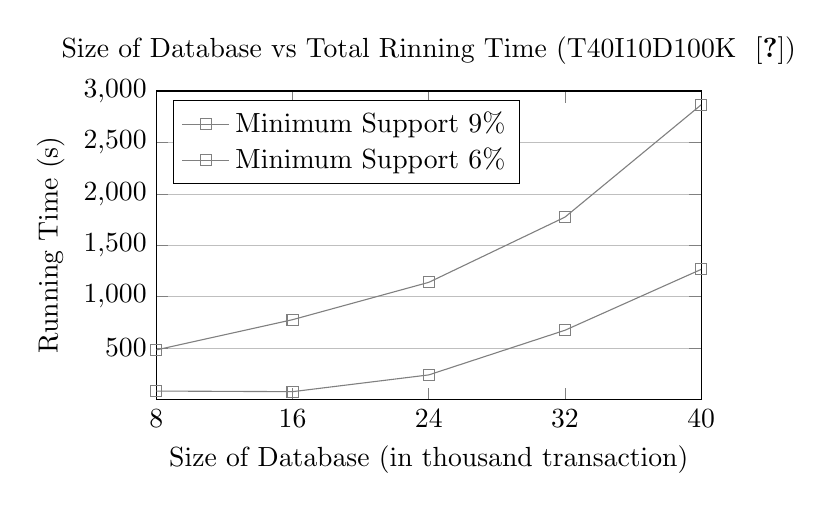
\begin{tikzpicture}
\begin{axis}[
	title={Size of Database vs Total Rinning Time (T40I10D100K ~\cite{dataset})},
    width=8.5cm,
    height=5.5cm,
    xlabel={Size of Database (in thousand transaction)},
    ylabel={Running Time (s)},
    xmin=8, xmax=40,
    ymin=0, ymax=3000,
    xtick={8,16,24,32,40},
    ytick={500,1000,1500,2000,2500,3000},
    legend pos=north west,
    ymajorgrids=true,
    grid style={line width=.2pt,draw=gray!50},
]
 
\addplot[
    solid,color=gray, every mark/.append style={solid, fill=gray}, mark=square
    ]
    coordinates {
			(8,482)
			(16,776)
			(24,1139)
			(32,1773)
			(40,2865)

	};
    \addlegendentry{Minimum Support 9\%}

\addplot[
    solid,color=gray, every mark/.append style={solid, fill=gray}, mark=square
    ]
    coordinates {
			(8,82)
			(16,76)
			(24,239)
			(32,673)
			(40,1265)

	};
    \addlegendentry{Minimum Support 6\%}

\end{axis}
\end{tikzpicture}
%\end{document}
        \caption{Size of Database vs Runtime for T40I10D100K ~\cite{dataset} Dataset }
        \label{result:g_t10_const_tran}
        \end{figure}
    
    \begin{table}[h]
        \centering
        \begin{tabular}{|c|c|}
        \hline 
       Size of Database        &    Memory (in MB)\\    \hline\hline
        
        1000&0.473\\\hline
        2000&0.795\\\hline
        3000&1.135\\\hline
        4000&1.442\\\hline
        5000&1.762\\\hline
    
            \end{tabular}
        \caption{ Total Memory (in MB) in Tree for Mushroom ~\cite{dataset} Dataset}
        \label{result:g_m_const_tran_mem}
        \end{table}
    
    \begin{table}[h]
        \centering
        \begin{tabular}{|c|c|}
        \hline 
       Size of Database       &    Memory (in MB)\\    \hline\hline
        
        8000 &23.504\\\hline
        10000&46.736\\\hline
        24000&69.861\\\hline
        32000&92.903\\\hline
        40000&115.888\\\hline
    
            \end{tabular}
        \caption{ Total Memory (in MB) in Tree for T40I10D100K ~\cite{dataset} Dataset}
        \label{result:g_t10_const_tran_mem}
        \end{table}

\paragraph{Window Size Change Effect}For window size change effect we have experimented our algorithm in the different angle. The experiment shows the window size change effect do not hamper performance and it is consistent. Figure-\ref{result:g_m_const_batch} and figure-\ref{result:g_t10_const_batch} shows effect of window size change effect on mushroom and T40I10D100K dataset.

        \begin{figure}[h]
        \centering
            %mark = star, diamond, square, otimes
%\documentclass{article}
%\usepackage{pgfplots}
%\usepackage[justification=centering]{caption}
%\pgfplotsset{compat=newest}
%\begin{document}
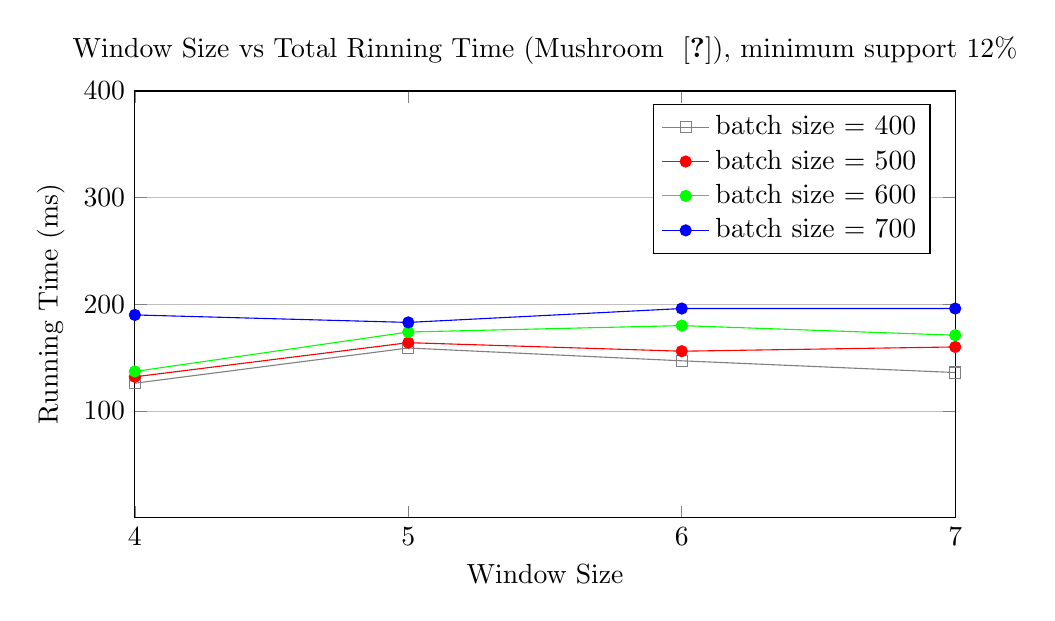
\begin{tikzpicture}
\begin{axis}[
 title={Window Size vs Total Rinning Time (Mushroom ~\cite{dataset}), minimum support 12\%},
 width=12cm,
   height=7cm,
    xlabel={Window Size},
	    ylabel={Running Time (ms)},
    xmin=4, xmax=7,
    ymin=0, ymax=400,
    xtick={4,5,6,7},
    ytick={100,200,300,400},
    legend pos=north east,
    ymajorgrids=true,
    grid style={line width=.2pt,draw=gray!50},
]
 
\addplot[
    solid,color=gray, every mark/.append style={solid, fill=gray}, mark=square
    ]
    coordinates {
			(4,126)			
			(5,159)			
			(6,147)			
			(7,136)
	};
    \addlegendentry{batch size $=$ 400}

	\addplot[
    solid,color=red, every mark/.append style={solid, fill=red}, mark=*
    ]
    coordinates {
			(4,132)			
			(5,164)			
			(6,156)			
			(7,160)
};
    \addlegendentry{batch size $=$ 500}
	

\addplot[
    solid,color=green, every mark/.append style={solid, fill=green}, mark=*
    ]
    coordinates {
			(4,137)			
			(5,174)			
			(6,180)			
			(7,171)
};
    \addlegendentry{batch size $=$ 600}
	
	
\addplot[
    solid,color=blue, every mark/.append style={solid, fill=blue}, mark=*
    ]
    coordinates {
			(4,190)			
			(5,183)			
			(6,196)			
			(7,196)
};
    \addlegendentry{batch size = 700}
\end{axis}
\end{tikzpicture}
%\end{document}
        \caption{Batch Size vs Runtime for Mushroom ~\cite{dataset} Dataset }
        \label{result:g_m_const_batch}
        \end{figure}
        \begin{figure}[h]
        \centering
            %mark = star, diamond, square, otimes
%\documentclass{article}
%\usepackage{pgfplots}
%\usepackage[justification=centering]{caption}
%\pgfplotsset{compat=newest}
%\begin{document}
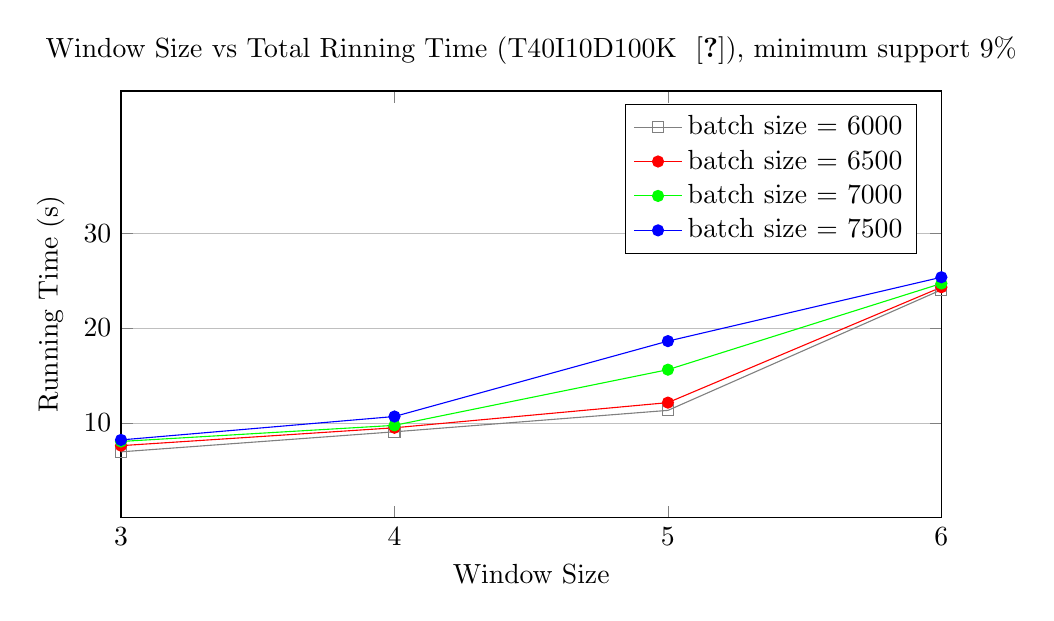
\begin{tikzpicture}
\begin{axis}[
 title={Window Size vs Total Rinning Time (T40I10D100K ~\cite{dataset}), minimum support 9\%},
 width=12cm,
   height=7cm,
    xlabel={Window Size},
    ylabel={Running Time (s)},
    xmin=3, xmax=6,
    ymin=0, ymax=45,
    xtick={3,4,5,6},
    ytick={10,20,30},
    legend pos=north east,
    ymajorgrids=true,
    grid style={line width=.2pt,draw=gray!50},
]
 
\addplot[
    solid,color=gray, every mark/.append style={solid, fill=gray}, mark=square
    ]
    coordinates {
		(3,6.935 )
		(4,9.048 )
		(5,11.308)
		(6,24.026)

	};
    \addlegendentry{batch size $=$ 6000}

	\addplot[
    solid,color=red, every mark/.append style={solid, fill=red}, mark=*
    ]
    coordinates {
		(3,7.587)
		(4,9.473)
		(5,12.126)
		(6,24.299)
};
    \addlegendentry{batch size $=$ 6500}
	

\addplot[
    solid,color=green, every mark/.append style={solid, fill=green}, mark=*
    ]
    coordinates {
		(3,8.030)
		(4,9.729)
		(5,15.602)
		(6,24.690)

};
    \addlegendentry{batch size $=$ 7000}
	
	
\addplot[
    solid,color=blue, every mark/.append style={solid, fill=blue}, mark=*
    ]
    coordinates {
		(3,8.192)
		(4,10.662)
		(5,18.613)
		(6,25.351)
};
    \addlegendentry{batch size $=$ 7500}
\end{axis}
\end{tikzpicture}
%\end{document}
        \caption{Batch Size vs Runtime for T40I10D100K ~\cite{dataset} Dataset }
        \label{result:g_t10_const_batch}
        \end{figure}
        % \begin{figure}[h]
        % \centering
        %     %mark = star, diamond, square, otimes
%\documentclass{article}
%\usepackage{pgfplots}
%\usepackage[justification=centering]{caption}
%\pgfplotsset{compat=newest}
%\begin{document}
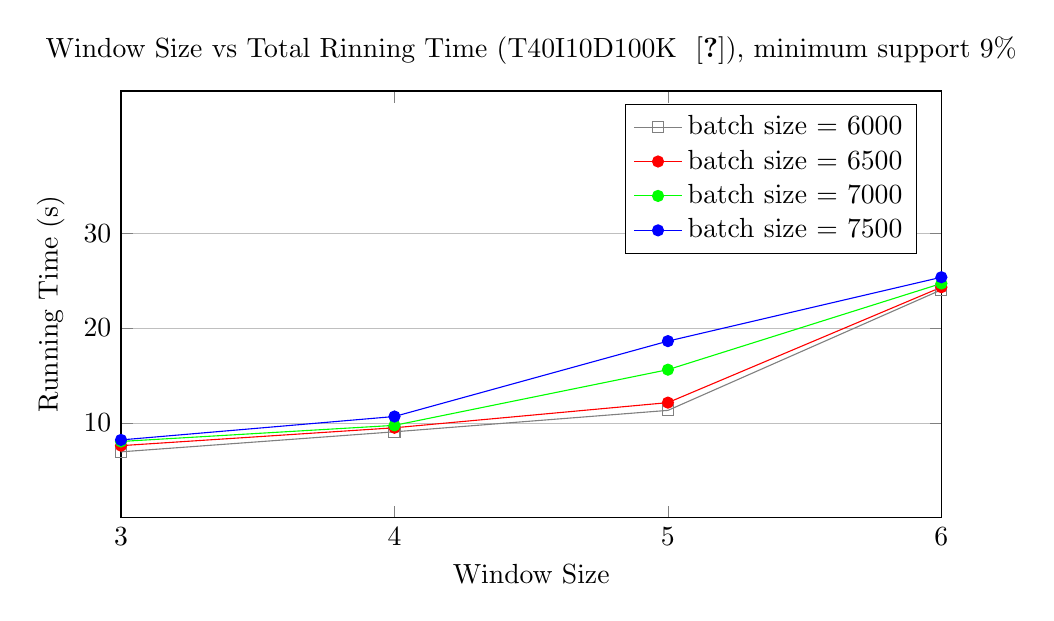
\begin{tikzpicture}
\begin{axis}[
 title={Window Size vs Total Rinning Time (T40I10D100K ~\cite{dataset}), minimum support 9\%},
 width=12cm,
   height=7cm,
    xlabel={Window Size},
    ylabel={Running Time (s)},
    xmin=3, xmax=6,
    ymin=0, ymax=45,
    xtick={3,4,5,6},
    ytick={10,20,30},
    legend pos=north east,
    ymajorgrids=true,
    grid style={line width=.2pt,draw=gray!50},
]
 
\addplot[
    solid,color=gray, every mark/.append style={solid, fill=gray}, mark=square
    ]
    coordinates {
		(3,6.935 )
		(4,9.048 )
		(5,11.308)
		(6,24.026)

	};
    \addlegendentry{batch size $=$ 6000}

	\addplot[
    solid,color=red, every mark/.append style={solid, fill=red}, mark=*
    ]
    coordinates {
		(3,7.587)
		(4,9.473)
		(5,12.126)
		(6,24.299)
};
    \addlegendentry{batch size $=$ 6500}
	

\addplot[
    solid,color=green, every mark/.append style={solid, fill=green}, mark=*
    ]
    coordinates {
		(3,8.030)
		(4,9.729)
		(5,15.602)
		(6,24.690)

};
    \addlegendentry{batch size $=$ 7000}
	
	
\addplot[
    solid,color=blue, every mark/.append style={solid, fill=blue}, mark=*
    ]
    coordinates {
		(3,8.192)
		(4,10.662)
		(5,18.613)
		(6,25.351)
};
    \addlegendentry{batch size $=$ 7500}
\end{axis}
\end{tikzpicture}
%\end{document}
        % \caption{Batch Size vs Runtime for T40I10D100K Dataset }
        % \label{result:g_t10_const_batch}
        % \end{figure}
         
\paragraph{Batch Size Change Effect}Like batch change effect we also experimented for batch size change effect.For changing batch size in different volume the result we find is consistent. For constant window and variable batches we have simulated our proposed algorithms. Figure-\ref{result:g_m_const_batch} and figure-\ref{result:g_t10_const_batch} shows effect of batch size change effect on mushroom and T40I10D100K dataset.
        \begin{figure}[h]
        \centering
            %mark = star, diamond, square, otimes
%\documentclass{article}
%\usepackage{pgfplots}
%\usepackage[justification=centering]{caption}
%\pgfplotsset{compat=newest}
%\begin{document}
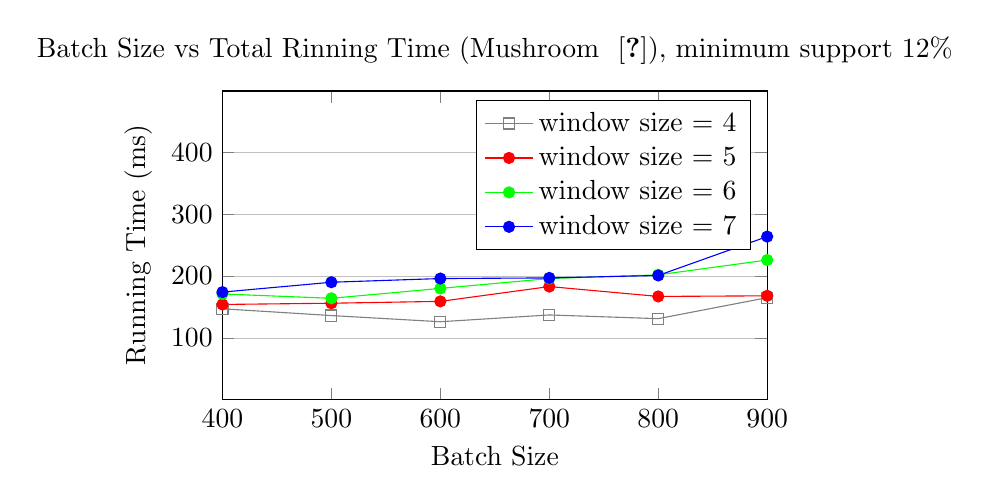
\begin{tikzpicture}
\begin{axis}[
 title={Batch Size vs Total Rinning Time (Mushroom ~\cite{dataset}), minimum support 12\%},
    width=8.5cm,
    height=5.5cm,
    xlabel={Batch Size},
    ylabel={Running Time (ms)},
    xmin=400, xmax=900,
    ymin=0, ymax=500,
    xtick={400,500,600,700,800,900},
    ytick={100,200,300,400},
    legend pos=north east,
    ymajorgrids=true,
    grid style={line width=.2pt,draw=gray!50},
]
 
\addplot[
    solid,color=gray, every mark/.append style={solid, fill=gray}, mark=square
    ]
    coordinates {
			(400,147)
			(500,136)
			(600,126)
			(700,137)
			(800,131)
			(900,165)
	};
    \addlegendentry{window size $=$ 4}

	\addplot[
    solid,color=red, every mark/.append style={solid, fill=red}, mark=*
    ]
    coordinates {
			(400,154)
			(500,156)
			(600,159)
			(700,183)
			(800,167)
			(900,168)
};
    \addlegendentry{window size $=$ 5}
	

\addplot[
    solid,color=green, every mark/.append style={solid, fill=green}, mark=*
    ]
    coordinates {
			(400,171)
			(500,164)
			(600,180)
			(700,196)
			(800,202)
			(900,226)
};
    \addlegendentry{window size $=$ 6}
	
	
\addplot[
    solid,color=blue, every mark/.append style={solid, fill=blue}, mark=*
    ]
    coordinates {
			(400,174)
			(500,190)
			(600,196)
			(700,197)
			(800,201)
			(900,264)
};
    \addlegendentry{window size = 7}
\end{axis}
\end{tikzpicture}
%\end{document}
        \caption{Window Size vs Runtime for Mushroom ~\cite{dataset} Dataset }
        \label{result:g_m_const_win}
        \end{figure}
        \begin{figure}[h]
        \centering
            %mark = star, diamond, square, otimes
%\documentclass{article}
%\usepackage{pgfplots}
%\usepackage[justification=centering]{caption}
%\pgfplotsset{compat=newest}
%\begin{document}
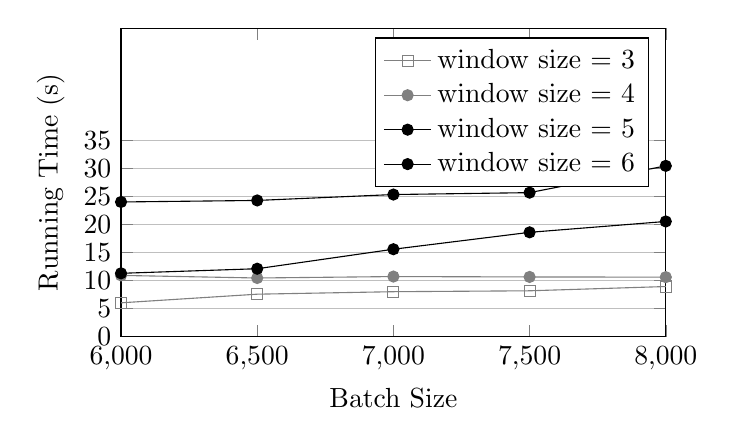
\begin{tikzpicture}
\begin{axis}[
    width=8.5cm,
    height=5.5cm,
    xlabel={Batch Size},
    ylabel={Running Time (s)},
    xmin=6000, xmax=8000,
    ymin=0, ymax=55,
    xtick={6000,6500,7000,7500,8000},
    ytick={0,5,10,15,20,25,30,35},
    legend pos=north east,
    ymajorgrids=true,
    grid style={line width=.2pt,draw=gray!50},
]
 
\addplot[
    solid,color=gray, every mark/.append style={solid, fill=gray}, mark=square
    ]
    coordinates {
		(6000,6.048)
		(6500,7.587 )
		(7000,8.030 )
		(7500,8.192 )
		(8000,8.951 )
	};
    \addlegendentry{window size $=$ 3}

	\addplot[
    solid,color=gray, every mark/.append style={solid, fill=gray}, mark=*
    ]
    coordinates {
		(6000,10.935)
		(6500,10.473)
		(7000,10.729)
		(7500,10.662)
		(8000,10.625)

};
    \addlegendentry{window size $=$ 4}
	

\addplot[
    solid,color=black, every mark/.append style={solid, fill=black}, mark=*
    ]
    coordinates {
		(6000,11.308)
		(6500,12.126)
		(7000,15.602)
		(7500,18.613)
		(8000,20.552)

};
    \addlegendentry{window size $=$ 5}
	
	
\addplot[
    solid,color=black, every mark/.append style={solid, fill=black}, mark=*
    ]
    coordinates {
		(6000,24.026)
		(6500,24.299)
		(7000,25.351)
		(7500,25.690)
		(8000,30.460)

};
    \addlegendentry{window size $=$ 6}
\end{axis}
\end{tikzpicture}
%\end{document}
        \caption{Window Size vs Runtime for T40I10D100K ~\cite{dataset} Dataset }
        \label{result:g_t10_const_win}
        \end{figure}
        
\subsection{Comparison With Existing Approaches}
Here now we have compared our proposed approach with existing system. We have choose SUF-growth ~\cite{suf_growth}  for comparison. This algorithm is perfectly fit for uncertain stream data mining. UF-streaming also designed for mining frequent patterns from uncertain stream but in ~\cite{suf_growth} it has been proved that in all criteria (runtime, memory and correctness) SUF-growth ~\cite{suf_growth} is better than UF-streaming ~\cite{suf_growth}. We have experimented for both runtime performance and memory efficiency. The result has described below:

\subsubsection{Runtime Comparison}
    Runtime comparison has been experimented and the in the result we found is consistent and we have gained runtime efficiency for both dense and sparse dataset. For mushroom dataset our approach's total tree construction time , total mining time and total time has been compared with SUF-growth ~\cite{suf_growth}'s tree construction time and mining time and total time. Figure-\ref{result:g_m_tree_construction_total}, figure-\ref{result:g_m_mining_total} and figure-\ref{result:g_m_total} shows the result graph. As mushroom is a dense database we gain much more in run time. For dense characteristic the constructed \emph{US-tree} is very much compact and moreover when mining compact tree the mining time surprisingly decreases that affect the total time. Figure-\ref{result:g_t10_tree_construction_total}, figure-\ref{result:g_t10_mining_total} and figure-\ref{result:g_t10_total} shows same comparison for T40I10D100K dataset . The graphs shows that our algorithm works correctly for sparse dataset too. Figure-\ref{result:g_chess_tree_construction_total}, figure-\ref{result:g_chess_mining_total} and figure-\ref{result:g_chess_total} shows tree construction time, mining time and total time for chess dataset. Kosarak is very large and real-life data set. This is web click database. This database is sparse and very much large. \ref{result:g_k_tree_construction_total}, figure-\ref{result:g_k_mining_total} and figure-\ref{result:g_k_total} shows the effect of changing minimum support effect corresponding to tree construction time, mining time and total time. This one is dense dataset and the result is consistent, efficient and also scalable.
            \begin{figure}[h]
            \centering
                %%mark = star, diamond, square, otimes
%\documentclass{article}
%\usepackage{pgfplots}
%\usepackage[justification=centering]{caption}
%\pgfplotsset{compat=newest}
%\begin{document} 
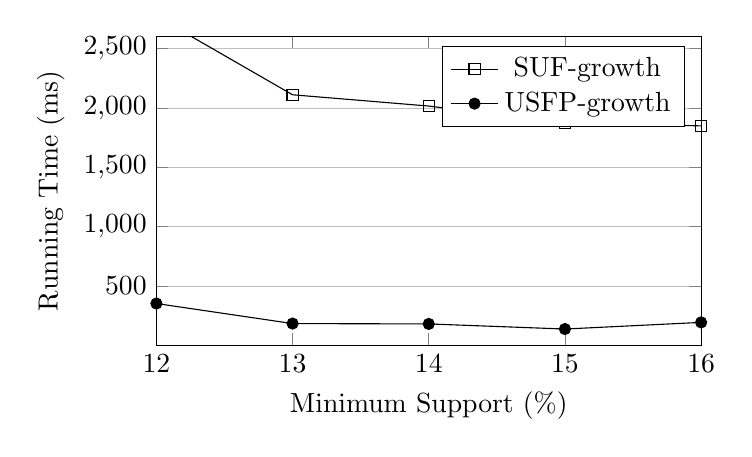
\begin{tikzpicture}
\begin{axis}[
    width=8.5cm,
    height=5.5cm,
    xlabel={Minimum Support (\%) },
    ylabel={Running Time (ms)},
    xmin=12, xmax=16,
    ymin=0, ymax=2600,
    xtick={12,13,14,15,16},
    ytick={500,1000,1500,2000,2500},
    legend pos=north east,
    ymajorgrids=true,
    grid style={line width=.2pt,draw=gray!50},
]
 
\addplot[
    solid, every mark/.append style={solid, fill=gray}, mark=square
    ]
    coordinates {
	(12,2771)
	(13,2110)
	(14,2015)
	(15,1873)
	(16,1848)

	};
    \addlegendentry{SUF-growth}
\addplot[
    solid, every mark/.append style={solid, fill=black}, mark=*
    ]
    coordinates {
	(12,351)
	(13,182)
	(14,179)
	(15,136)
	(16,192)

};
    \addlegendentry{USFP-growth}
 
\end{axis}
\end{tikzpicture}
%\end{document}
            \caption{Total Tree Construction Time vs Minimum Support(\%) for Mushroom ~\cite{dataset} Dataset }
            \label{result:g_m_tree_construction_total}
            \end{figure}
            
            \begin{figure}[h]
            \centering
                %%mark = star, diamond, square, otimes
%\documentclass{article}
%\usepackage{pgfplots}
%\usepackage[justification=centering]{caption}
%\pgfplotsset{compat=newest}
%\begin{document}
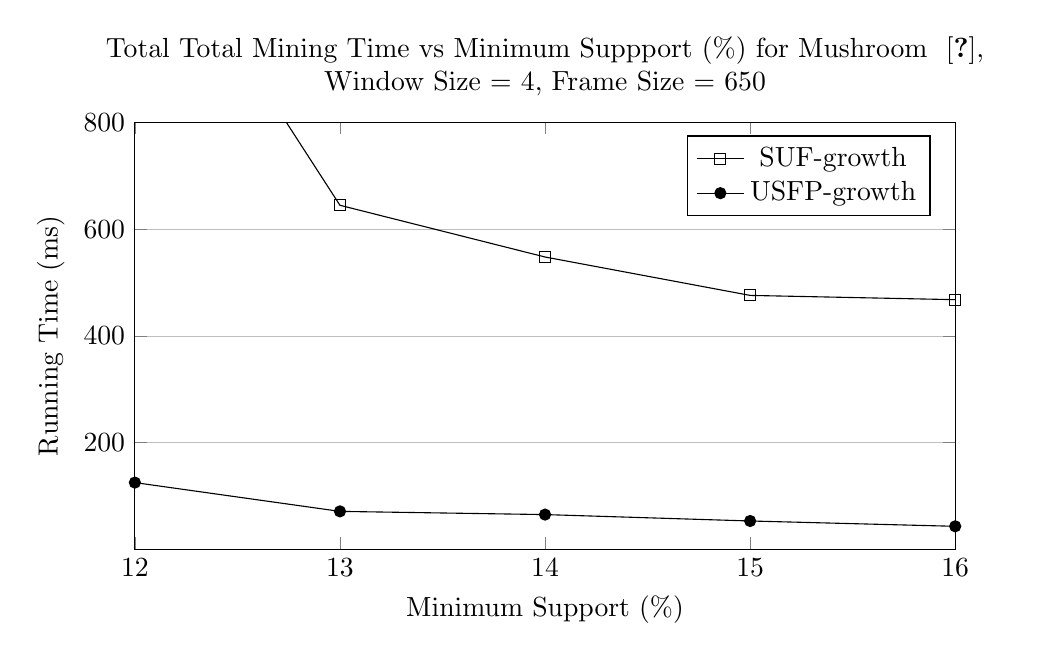
\begin{tikzpicture}
\begin{axis}[
	title={\parbox{\linewidth}{\centering Total Total Mining Time vs Minimum Suppport (\%) for Mushroom ~\cite{dataset}, Window Size = 4, Frame Size = 650}},
	width=12cm,
	height=7cm,
    xlabel={Minimum Support (\%) },
    ylabel={Running Time (ms)},
    xmin=12, xmax=16,
    ymin=0, ymax=800,
    xtick={12,13,14,15,16},
    ytick={200,400,600,800},
    legend pos=north east,
    ymajorgrids=true,
    grid style={line width=.2pt,draw=gray!50},
]
 
\addplot[
    solid, every mark/.append style={solid, fill=gray}, mark=square
    ]
    coordinates {
	(12,1240)
	(13,645)
	(14,548)
	(15,476)
	(16,468)

};
    \addlegendentry{SUF-growth}
\addplot[
    solid, every mark/.append style={solid, fill=black}, mark=*
    ]
    coordinates {
	(12,125)
	(13,71 )
	(14,65 )
	(15,53 )
	(16,43 )

};
    \addlegendentry{USFP-growth}
 
\end{axis}
\end{tikzpicture}
%\end{document}
            \caption{Total Tree Mining Time vs Minimum Support(\%) for Mushroom ~\cite{dataset} Dataset }
            \label{result:g_m_mining_total}
            \end{figure}
            \begin{figure}[h]
            \centering
                %%mark = star, diamond, square, otimes
%\documentclass{article}
%\usepackage{pgfplots}
%\usepackage[justification=centering]{caption}
%\pgfplotsset{compat=newest}
%\begin{document}
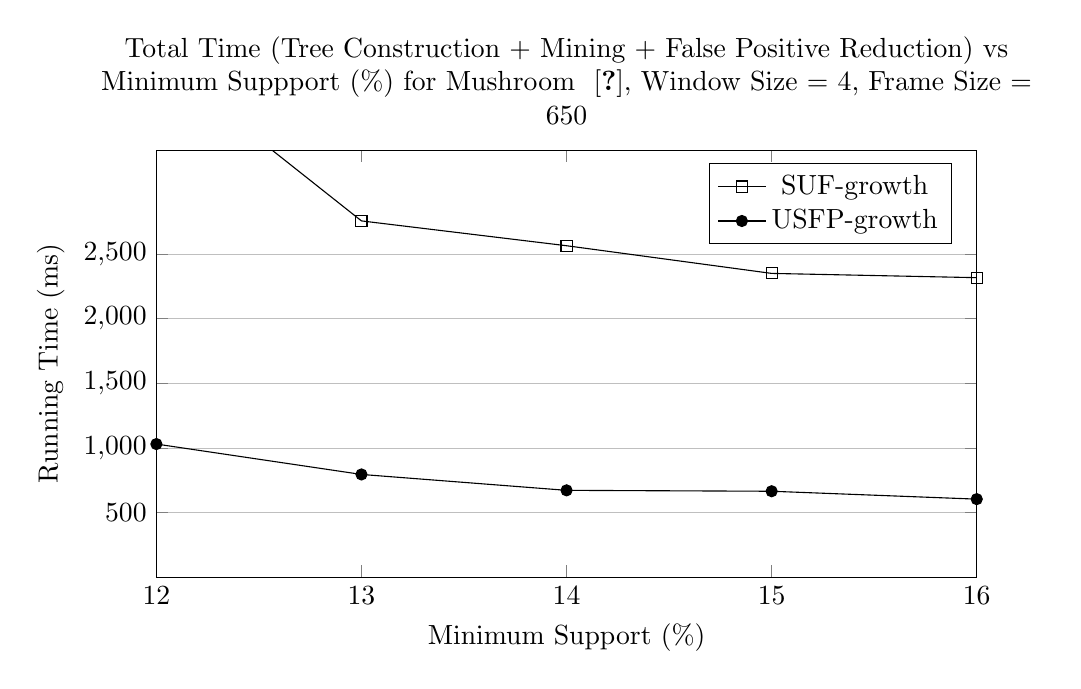
\begin{tikzpicture}
\begin{axis}[
	title={\parbox{\linewidth}{\centering Total Time (Tree Construction + Mining + False Positive Reduction) vs Minimum Suppport (\%) for Mushroom ~\cite{dataset}, Window Size = 4, Frame Size = 650}},
	width=12cm,
	height=7cm,
    xlabel={Minimum Support (\%) },
    ylabel={Running Time (ms)},
    xmin=12, xmax=16,
    ymin=0, ymax=3300,
    xtick={12,13,14,15,16},
    ytick={500,1000,1500,2000,2500},
    legend pos=north east,
    ymajorgrids=true,
    grid style={line width=.2pt,draw=gray!50},
]
 
\addplot[
    solid, every mark/.append style={solid, fill=gray}, mark=square
    ]
    coordinates {
	(12,4011)
	(13,2755)
	(14,2563)
	(15,2349)
	(16,2316)

};
    \addlegendentry{SUF-growth}
\addplot[
    solid, every mark/.append style={solid, fill=black}, mark=*
    ]
    coordinates {
	(12,1029)
	(13,794)
	(14,671)
	(15,664)
	(16,603)

};
    \addlegendentry{USFP-growth}
 
\end{axis}
\end{tikzpicture}
%\end{document}
            \caption{Runtime vs Minimum Support(\%) for Mushroom ~\cite{dataset} Dataset }
            \label{result:g_m_total}
            \end{figure}
            \begin{figure}[h]
            \centering
                %%mark = star, diamond, square, otimes
%\documentclass{article}
%\usepackage{pgfplots}
%\usepackage[justification=centering]{caption}
%\pgfplotsset{compat=newest} 	title={\parbox{\linewidth}{\centering Total Tree Construction Time vs Minimum Suppport (\%) for T40I10D100K ~\cite{dataset}, Window Size = 5, Frame Size = 7000}},
%\begin{document}
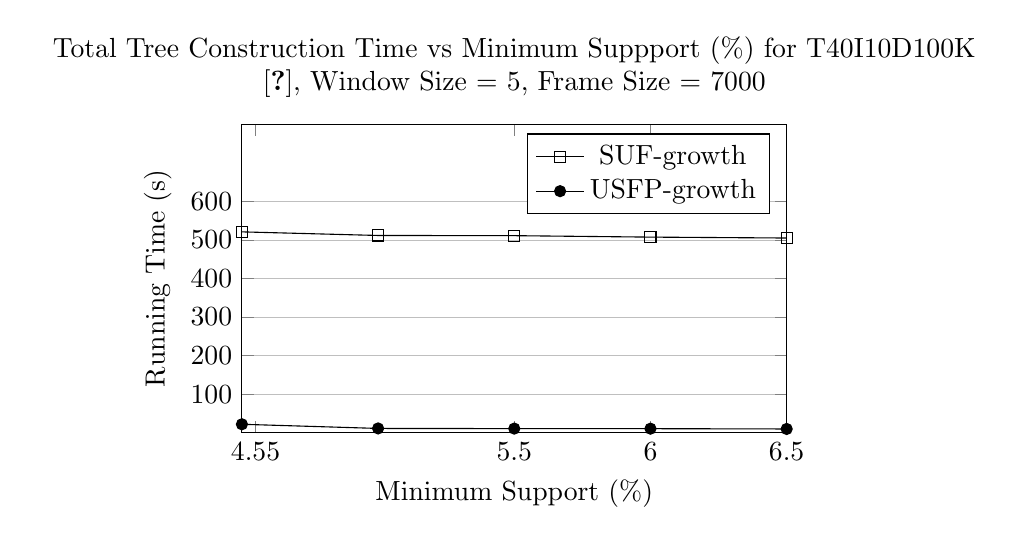
\begin{tikzpicture}
	\begin{axis}[
	title={\parbox{\linewidth}{\centering Total Tree Construction Time vs Minimum Suppport (\%) for T40I10D100K ~\cite{dataset}, Window Size = 5, Frame Size = 7000}},
    width=8.5cm,
    height=5.5cm,
    xlabel={Minimum Support (\%) },
    ylabel={Running Time (s)},
    xmin=4.5, xmax=6.5,
    ymin=0, ymax=800,
    xtick={4.55,5.5,6,6.5},
    ytick={100,200,300,400,500,600},
    legend pos=north east,
    ymajorgrids=true,
    grid style={line width=.2pt,draw=gray!50},
]
 
\addplot[
    solid, every mark/.append style={solid, fill=gray}, mark=square
    ]
    coordinates {
			(4.5,520.723)
			(5  ,511.365)
			(5.5,510.854)
			(6  ,507.12 )
			(6.5,504.767)


	};
    \addlegendentry{SUF-growth}
\addplot[
    solid, every mark/.append style={solid, fill=black}, mark=*
    ]
    coordinates {
		(4.5,21.814)
		(5  ,11.035)
		(5.5,10.601)
		(6  ,10.423)
		(6.5,9.646 )


};
    \addlegendentry{USFP-growth}
 
\end{axis}
\end{tikzpicture}
%\end{document}
            \caption{Total Tree Construction Time vs Minimum Support(\%) for T40I10D100K ~\cite{dataset} Dataset }
            \label{result:g_t10_tree_construction_total}
            \end{figure}
            
            \begin{figure}[h]
            \centering
                %%%mark = star, diamond, square, otimes
%\documentclass{article}
%\usepackage{pgfplots}
%\usepackage[justification=centering]{caption}
%\pgfplotsset{compat=newest}
%\begin{document}
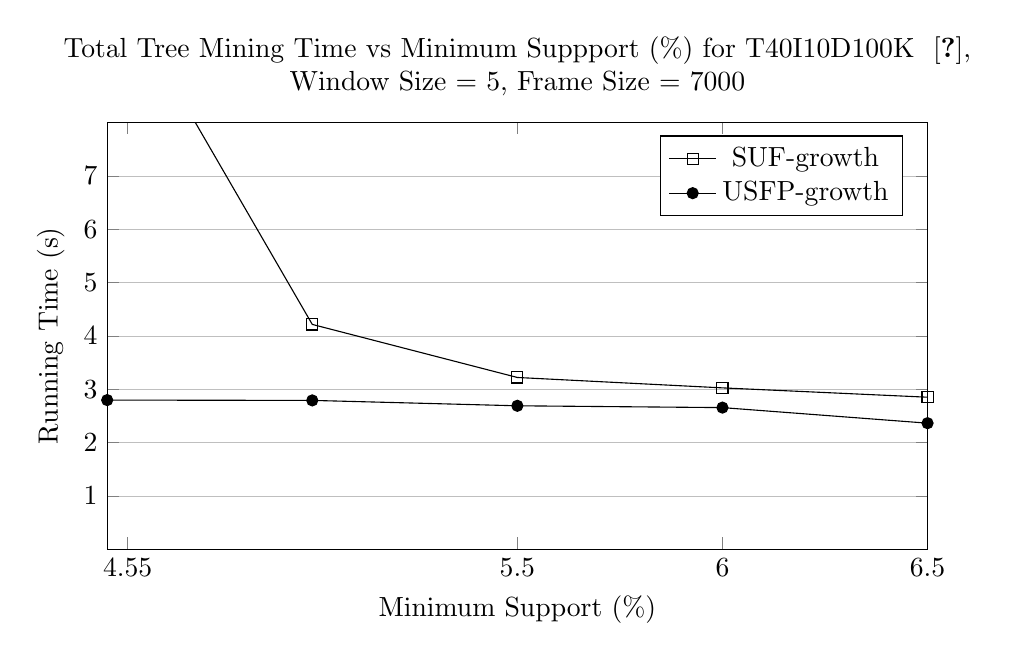
\begin{tikzpicture}
\begin{axis}[
	title={\parbox{\linewidth}{\centering Total Tree Mining Time vs Minimum Suppport (\%) for T40I10D100K ~\cite{dataset}, Window Size = 5, Frame Size = 7000}},
	width=12cm,
	height=7cm,
    xlabel={Minimum Support (\%) },
    ylabel={Running Time (s)},
    xmin=4.5, xmax=6.5,
    ymin=0, ymax=8,
    xtick={4.55,5.5,6,6.5},
    ytick={1,2,3,4,5,6,7},
    legend pos=north east,
    ymajorgrids=true,
    grid style={line width=.2pt,draw=gray!50},
]
 
\addplot[
    solid, every mark/.append style={solid, fill=gray}, mark=square
    ]
    coordinates {
			(4.5,10.856)
			(5  ,4.216 )
			(5.5,3.221 )
			(6  ,3.026 )
			(6.5,2.851 )


};
    \addlegendentry{SUF-growth}
\addplot[
    solid, every mark/.append style={solid, fill=black}, mark=*
    ]
    coordinates {
			(4.5,  2.797)
			(5  , 2.791)
			(5.5,2.69 )
			(6  ,2.656 )
			(6.5,2.364 )


};
    \addlegendentry{USFP-growth}
 
\end{axis}
\end{tikzpicture}
%\end{document}
            \caption{Total Tree Mining Time vs Minimum Support(\%) for T40I10D100K ~\cite{dataset} Dataset }
            \label{result:g_t10_mining_total}
            \end{figure}
            
            \begin{figure}[h]
            \centering
                %%%mark = star, diamond, square, otimes
%\documentclass{article}
%\usepackage{pgfplots}
%\usepackage[justification=centering]{caption}
%\pgfplotsset{compat=newest}
%\begin{document}
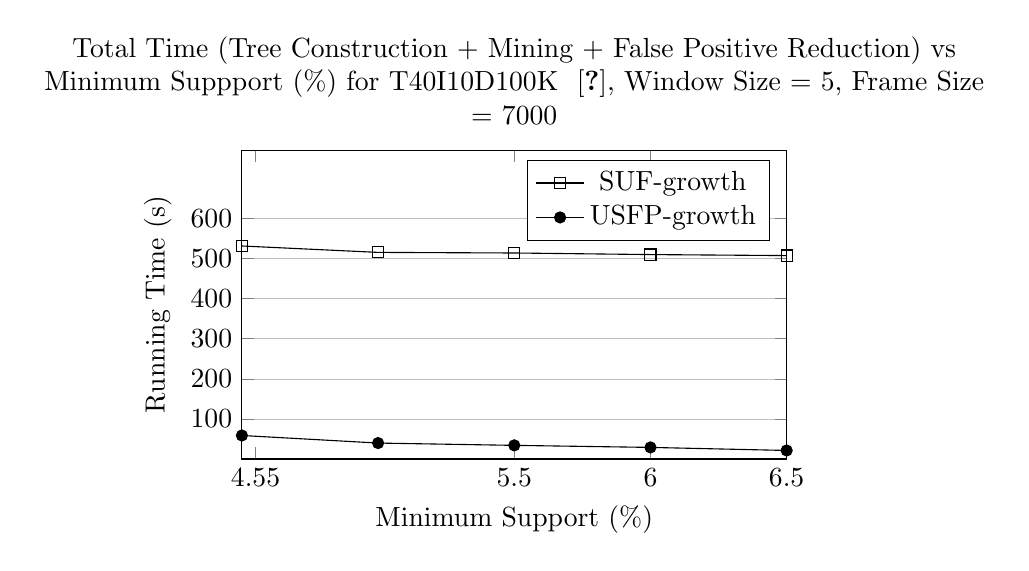
\begin{tikzpicture}
\begin{axis}[
	title={\parbox{\linewidth}{\centering  Total Time (Tree Construction + Mining + False Positive Reduction) vs Minimum Suppport (\%) for T40I10D100K ~\cite{dataset}, Window Size = 5, Frame Size = 7000}},
    width=8.5cm,
    height=5.5cm,
    xlabel={Minimum Support (\%) },
    ylabel={Running Time (s)},
    xmin=4.5, xmax=6.5,
    ymin=0, ymax=770,
    xtick={4.55,5.5,6,6.5},
    ytick={100,200,300,400,500,600},
    legend pos=north east,
    ymajorgrids=true,
    grid style={line width=.2pt,draw=gray!50},
]
 
\addplot[
    solid, every mark/.append style={solid, fill=gray}, mark=square
    ]
    coordinates {
			(4.5,531.579)
			(5  ,515.581)
			(5.5,514.075)
			(6  ,510.146)
			(6.5,507.618)

};
    \addlegendentry{SUF-growth}
\addplot[
    solid, every mark/.append style={solid, fill=black}, mark=*
    ]
    coordinates {
			(4.5,58.652)
			(5  ,39.735)
			(5.5,33.993)
			(6  ,28.892)
			(6.5,21.262)


};
    \addlegendentry{USFP-growth}
 
\end{axis}
\end{tikzpicture}
%\end{document}
            \caption{Runtime vs Minimum Support(\%) for T40I10D100K ~\cite{dataset} Dataset }
            \label{result:g_t10_total}
            \end{figure}
    
            \begin{figure}[h]
            \centering
                %%mark = star, diamond, square, otimes
%\documentclass{article}
%\usepackage{pgfplots}
%\usepackage[justification=centering]{caption}
%\pgfplotsset{compat=newest}
%\begin{document} 
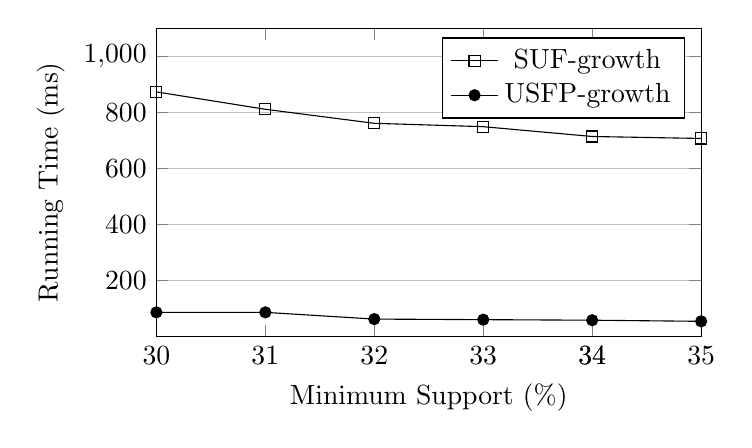
\begin{tikzpicture}
\begin{axis}[
    width=8.5cm,
    height=5.5cm,
    xlabel={Minimum Support (\%) },
    ylabel={Running Time (ms)},
    xmin=30, xmax=35,
    ymin=0, ymax=1100,
    xtick={30,31,32,33,34,34,35},
    ytick={200,400,600,800,1000},
    legend pos=north east,
    ymajorgrids=true,
    grid style={line width=.2pt,draw=gray!50},
]
 
\addplot[
    solid, every mark/.append style={solid, fill=gray}, mark=square
    ]
    coordinates {
			(30,873)
			(31,811)
			(32,761)
			(33,749)
			(34,714)
			(35,707)

	};
    \addlegendentry{SUF-growth}
\addplot[
    solid, every mark/.append style={solid, fill=black}, mark=*
    ]
    coordinates {
			(30,87)
			(31,87)
			(32,63)
			(33,61)
			(34,59)
			(35,55)

};
    \addlegendentry{USFP-growth}
 
\end{axis}
\end{tikzpicture}
%\end{document}
            \caption{Total Tree Construction Time vs Minimum Support(\%) for Chess ~\cite{dataset} Dataset }
            \label{result:g_chess_tree_construction_total}
            \end{figure}
            
            \begin{figure}[h]
            \centering
                %%mark = star, diamond, square, otimes
%\documentclass{article}
%\usepackage{pgfplots}
%\usepackage[justification=centering]{caption}
%\pgfplotsset{compat=newest}
%\begin{document}
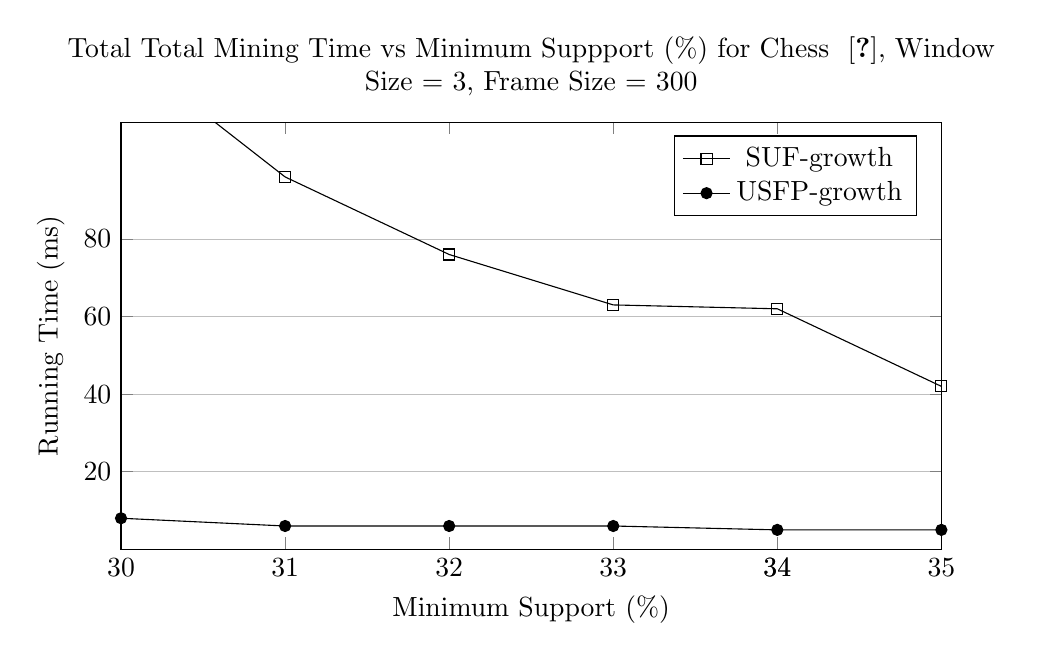
\begin{tikzpicture}
\begin{axis}[
	title={\parbox{\linewidth}{\centering Total Total Mining Time vs Minimum Suppport (\%) for Chess ~\cite{dataset}, Window Size = 3, Frame Size = 300}},
	width=12cm,
	height=7cm,
    xlabel={Minimum Support (\%) },
    ylabel={Running Time (ms)},
    xmin=30, xmax=35,
    ymin=0, ymax=110,
    xtick={30,31,32,33,34,34,35},
    ytick={20,40,60,80},
    legend pos=north east,
    ymajorgrids=true,
    grid style={line width=.2pt,draw=gray!50},
]
 
\addplot[
    solid, every mark/.append style={solid, fill=gray}, mark=square
    ]
    coordinates {
			(30,129)
			(31,96)
			(32,76)
			(33,63)
			(34,62)
			(35,42)

};
    \addlegendentry{SUF-growth}
\addplot[
    solid, every mark/.append style={solid, fill=black}, mark=*
    ]
    coordinates {
			(30,8)
			(31,6)
			(32,6)
			(33,6)
			(34,5)
			(35,5)

};
    \addlegendentry{USFP-growth}
 
\end{axis}
\end{tikzpicture}
%\end{document}
            \caption{Total Tree Mining Time vs Minimum Support(\%) for Chess ~\cite{dataset} Dataset }
            \label{result:g_chess_mining_total}
            \end{figure}
            
            \begin{figure}[h]
            \centering
                %%mark = star, diamond, square, otimes
%\documentclass{article}
%\usepackage{pgfplots}
%\usepackage[justification=centering]{caption}
%\pgfplotsset{compat=newest}
%\begin{document}
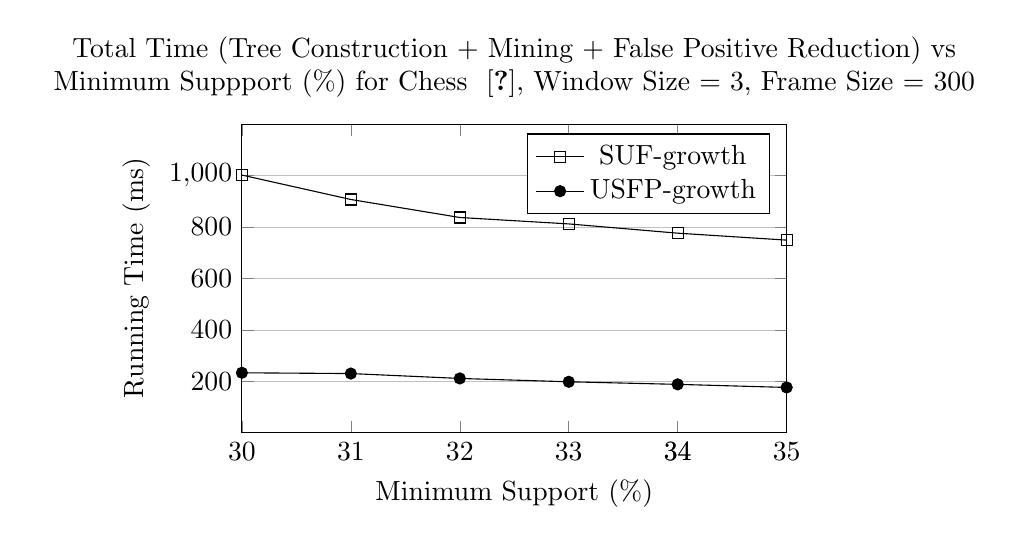
\begin{tikzpicture}
\begin{axis}[
	title={\parbox{\linewidth}{\centering Total Time (Tree Construction + Mining + False Positive Reduction) vs Minimum Suppport (\%) for Chess ~\cite{dataset}, Window Size = 3, Frame Size = 300}},
    width=8.5cm,
    height=5.5cm,
    xlabel={Minimum Support (\%) },
    ylabel={Running Time (ms)},
    xmin=30, xmax=35,
    ymin=0, ymax=1200,
    xtick={30,31,32,33,34,34,35},
    ytick={200,400,600,800,1000},
    legend pos=north east,
    ymajorgrids=true,
    grid style={line width=.2pt,draw=gray!50},
]
 
\addplot[
    solid, every mark/.append style={solid, fill=gray}, mark=square
    ]
    coordinates {
			(30,1002)
			(31,907)
			(32,837)
			(33,812)
			(34,776)
			(35,749)
};
    \addlegendentry{SUF-growth}
\addplot[
    solid, every mark/.append style={solid, fill=black}, mark=*
    ]
    coordinates {
			(30,233)
			(31,230)
			(32,211)
			(33,198)
			(34,188)
			(35,176)

};
    \addlegendentry{USFP-growth}
 
\end{axis}
\end{tikzpicture}
%\end{document}
            \caption{Runtime vs Minimum Support(\%) for Chess ~\cite{dataset} Dataset }
            \label{result:g_chess_total}
            \end{figure}
            \begin{figure}[h]
            \centering
                %%mark = star, diamond, square, otimes
%\documentclass{article}
%\usepackage{pgfplots}
%\usepackage[justification=centering]{caption}
%\pgfplotsset{compat=newest}
%\begin{document} 
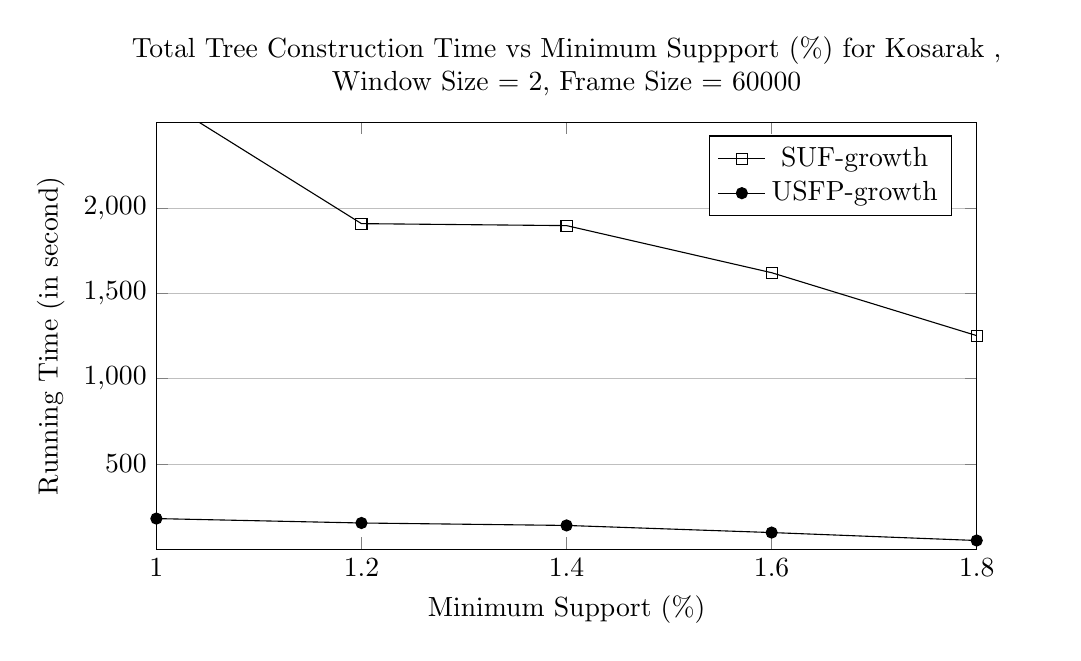
\begin{tikzpicture}
\begin{axis}[
	title={\parbox{\linewidth}{\centering Total Tree Construction Time vs Minimum Suppport (\%) for Kosarak , Window Size = 2, Frame Size = 60000}},
	width=12cm,
	height=7cm,
    xlabel={Minimum Support (\%) },
    ylabel={Running Time (in second)},
    xmin=1.0, xmax=1.8,
    ymin=0, ymax=2500,
    xtick={1.0,1.2,1.4,1.6,1.8},
    ytick={500,1000,1500,2000},
    legend pos=north east,
    ymajorgrids=true,
    grid style={line width=.2pt,draw=gray!50},
]
 
\addplot[
    solid, every mark/.append style={solid, fill=gray}, mark=square
    ]
    coordinates {
		(1.0 ,	2658.345	)
		(1.2,	1908.075	)
		(1.4,	1896.467	)
		(1.6,	1620.51		)
		(1.8,	1251.685	)	
		
	};
    \addlegendentry{SUF-growth}
\addplot[
    solid, every mark/.append style={solid, fill=black}, mark=*
    ]
    coordinates {
		(1.0  ,	179.797	)
		(1.2,	153.960	)
		(1.4,	139.599	)
		(1.6,	97.878	)
		(1.8,	51.297	)

};
    \addlegendentry{USFP-growth}
 
\end{axis}
\end{tikzpicture}
%\end{document}
            \caption{Total Tree Construction Time vs Minimum Support(\%) for Kosarak ~\cite{dataset} Dataset }
            \label{result:g_k_tree_construction_total}
            \end{figure}
            
            \begin{figure}[h]
            \centering
                %%mark = star, diamond, square, otimes
%\documentclass{article}
%\usepackage{pgfplots}
%\usepackage[justification=centering]{caption}
%\pgfplotsset{compat=newest}
%\begin{document}
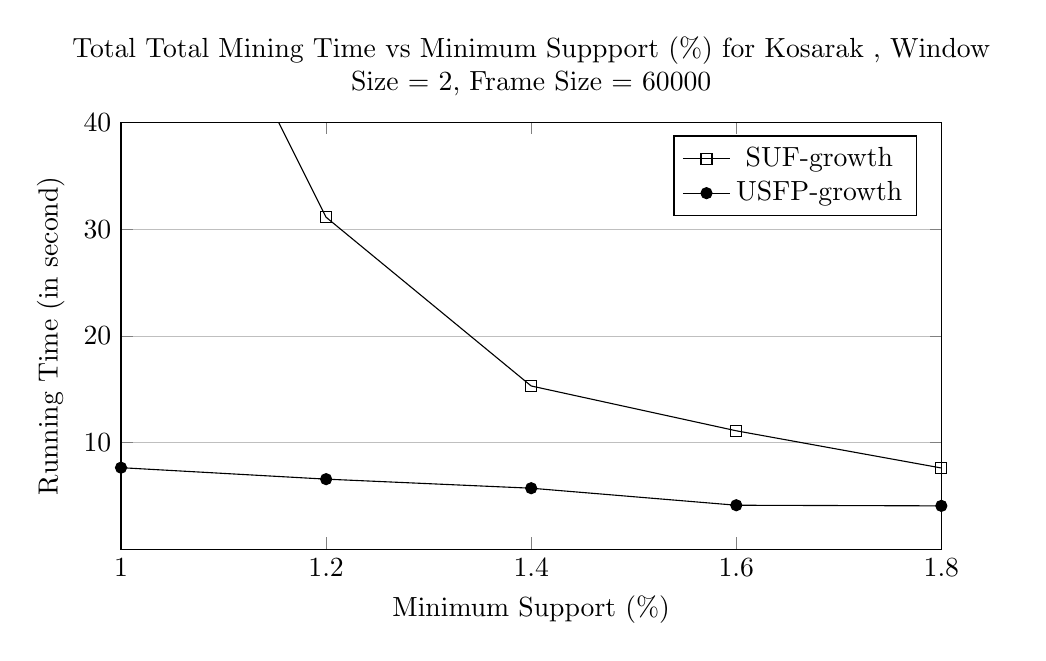
\begin{tikzpicture}
\begin{axis}[
	title={\parbox{\linewidth}{\centering Total Total Mining Time vs Minimum Suppport (\%) for Kosarak , Window Size = 2, Frame Size = 60000}},
	width=12cm,
	height=7cm,
    xlabel={Minimum Support (\%) },
    ylabel={Running Time (in second)},
    xmin=1.0, xmax=1.8,
    ymin=0, ymax=40,
    xtick={1.0,1.2,1.4,1.6,1.8},
    ytick={10,20,30,40},
    legend pos=north east,
    ymajorgrids=true,
    grid style={line width=.2pt,draw=gray!50},
]
 
\addplot[
    solid, every mark/.append style={solid, fill=gray}, mark=square
    ]
    coordinates {
		(1.0  ,	69.55)
		(1.2,	31.13)
		(1.4,	15.310)
		(1.6,	11.108)
		(1.8,	7.620)
};
    \addlegendentry{SUF-growth}
\addplot[
    solid, every mark/.append style={solid, fill=black}, mark=*
    ]
    coordinates {
		(1.0 ,	7.650	)
		(1.2,	6.575	)
		(1.4,	5.725	)
		(1.6,	4.128	)
		(1.8,	4.069	)
};
    \addlegendentry{USFP-growth}
 
\end{axis}
\end{tikzpicture}
%\end{document}
            \caption{Total Tree Mining Time vs Minimum Support(\%) for Kosarak ~\cite{dataset} Dataset }
            \label{result:g_k_mining_total}
            \end{figure}

            \begin{figure}[h]
            \centering
                %%mark = star, diamond, square, otimes
%\documentclass{article}
%\usepackage{pgfplots}
%\usepackage[justification=centering]{caption}
%\pgfplotsset{compat=newest}
%\begin{document}
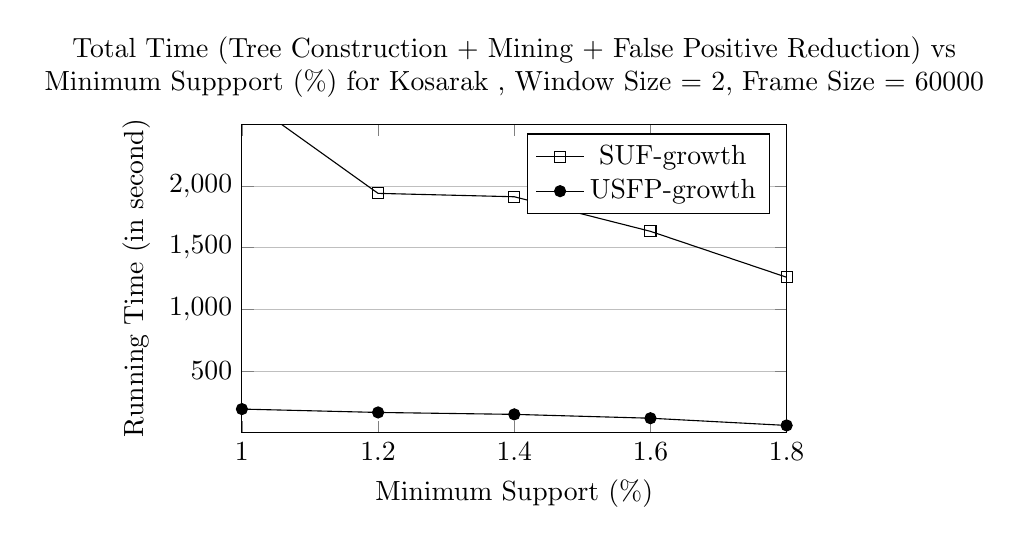
\begin{tikzpicture}
\begin{axis}[
	title={\parbox{\linewidth}{\centering Total Time (Tree Construction + Mining + False Positive Reduction) vs Minimum Suppport (\%) for Kosarak , Window Size = 2, Frame Size = 60000}},
    width=8.5cm,
    height=5.5cm,
    xlabel={Minimum Support (\%) },
    ylabel={Running Time (in second)},
    xmin=1.0, xmax=1.8,
    ymin=0, ymax=2500,
    xtick={1.0,1.2,1.4,1.6,1.8},
    ytick={500,1000,1500,2000},
    legend pos=north east,
    ymajorgrids=true,
    grid style={line width=.2pt,draw=gray!50},
]
 
\addplot[
    solid, every mark/.append style={solid, fill=gray}, mark=square
    ]
    coordinates {
		(1.0  ,	2727.895)
		(1.2,	1939.205)
		(1.4,	1911.777)
		(1.6,	1631.618)
		(1.8,	1259.305)
		
};
    \addlegendentry{SUF-growth}
\addplot[
    solid, every mark/.append style={solid, fill=black}, mark=*
    ]
    coordinates {
		(1.0 ,	191.309	)
		(1.2,	164.057	)
		(1.4,	148.466	)
		(1.6,	117.228	)
		(1.8,	58.768	)
};
    \addlegendentry{USFP-growth}
 
\end{axis}
\end{tikzpicture}
%\end{document}
            \caption{Runtime vs Minimum Support(\%) for Kosarak ~\cite{dataset} Dataset }
            \label{result:g_k_total}
            \end{figure}
            
\subsubsection{Memory Comparison}
As our proposed \emph{US-tree} have the capability to share nodes more than \emph{SUF-growth}, we get much more gain in memory. The experimental result also indicates that very clearly. Figure-\ref{result:g_m_memory_node} shows the memory comparison on mushroom dataset. Mushroom is the dense database so we get  much more gain in memory. The graph clearly shows that with the increase of total transaction in the tree gives the much more gain. For chess dataset the compactness of tree is also very impressive as this dataset is also compact (figure-\ref{result:g_chess_memory_node}) the Dense dataset have more scope to share nodes more. Figure-\ref{result:g_t10_memory_node} also shows that in T40I10D100K database we also gain the memory optimization. Figure-\ref{result:g_k_memory_node} shows memory comparison between \emph{USFP-growth} vs \emph{SUF-growth} ~\cite{suf_growth}. On this sparse database it has been clearly shown that, lot of memory optimization has been possible with our proposed algorithm. As the database is sparse, we get the memory gain less then dense one.
            \begin{figure}[h]
            \centering
                %mark = star, diamond, square, otimes
%\documentclass{article}
%\usepackage{pgfplots}
%\usepackage[justification=centering]{caption}
%\pgfplotsset{compat=newest}
%\begin{document}
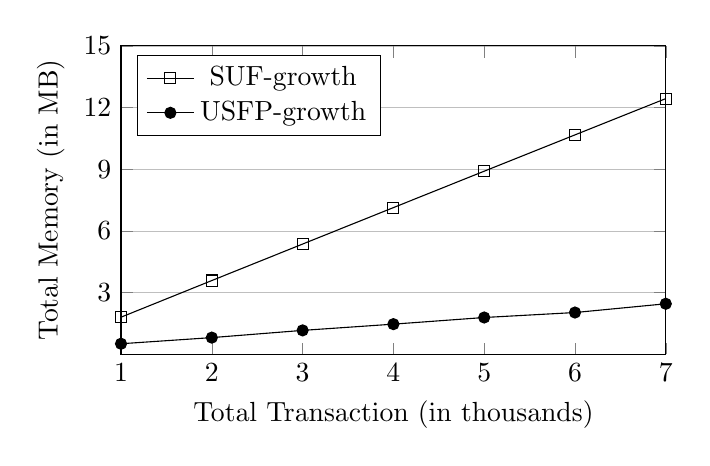
\begin{tikzpicture}
\begin{axis}[
	width=8.5cm,
	height=5.5cm,
    xlabel={Total Transaction (in thousands) },
    ylabel={Total Memory (in MB) },
    xmin=1, xmax=7,
    ymin=0, ymax=15,
    xtick={1,2,3,4,5,6,7},
    ytick={3,6,9,12,15},
    legend pos=north west,
    ymajorgrids=true,
    grid style={line width=.2pt,draw=gray!50},
]
 
\addplot[
    solid, every mark/.append style={solid, fill=gray}, mark=square
    ]
    coordinates {
			(1,1.807  )
			(2,3.588  )
			(3,5.362  )
			(4,7.134     )
			(5,8.905  )
			(6,10.670 )
			(7,12.434  )



	};
    \addlegendentry{SUF-growth}
\addplot[
    solid, every mark/.append style={solid, fill=black}, mark=*
    ]
    coordinates {
			(1,.5152  )
			(2,.814  )
			(3,1.165 )
			(4,1.468 )
			(5,1.791  )
			(6,2.033 )
			(7,2.458 )


};
    \addlegendentry{USFP-growth}
 
\end{axis}
\end{tikzpicture}
%\end{document}
            \caption{Total Memory vs Total Transaction (in thousand) for Mushroom ~\cite{dataset} Dataset }
            \label{result:g_m_memory_node}
            \end{figure}
            
            \begin{figure}[h]
            \centering
                %mark = star, diamond, square, otimes
%\documentclass{article}
%\usepackage{pgfplots}
%\usepackage[justification=centering]{caption}
%\pgfplotsset{compat=newest}
%\begin{document}
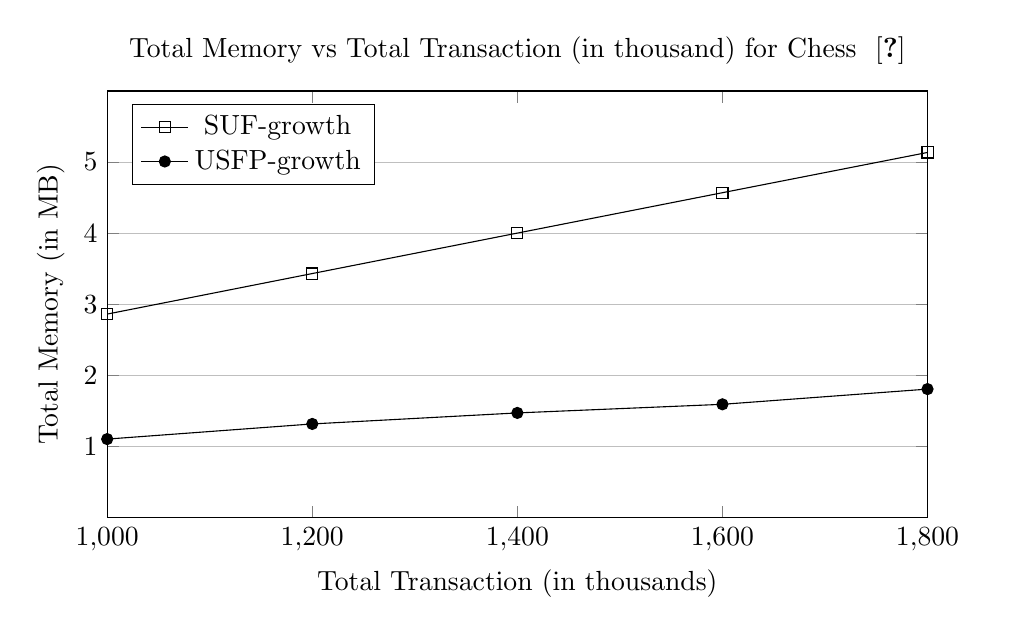
\begin{tikzpicture}
\begin{axis}[
	title={\parbox{\linewidth}{\centering Total Memory vs Total Transaction (in thousand) for Chess ~\cite{dataset}}},
	width=12cm,
	height=7cm,
    xlabel={Total Transaction (in thousands) },
    ylabel={Total Memory (in MB) },
    xmin=1000, xmax=1800,
    ymin=0, ymax=6,
    xtick={600,800,1000,1200,1400,1600,1800},
    ytick={1,2,3,4,5},
    legend pos=north west,
    ymajorgrids=true,
    grid style={line width=.2pt,draw=gray!50},
]
 
\addplot[
    solid, every mark/.append style={solid, fill=gray}, mark=square
    ]
    coordinates {
			(600,	1.720)
			(800,	2.291)
			(1000,	2.862)
			(1200,	3.432)
			(1400,	4.001)
			(1600,	4.569)
            (1800,	5.135)



	};
    \addlegendentry{SUF-growth}
\addplot[
    solid, every mark/.append style={solid, fill=black}, mark=*
    ]
    coordinates {
			(600,	0.681 )
			(800,	0.865 )
			(1000,	1.104 )
			(1200,	1.317 )
			(1400,	1.472 )
			(1600,	1.593 )
            (1800,	1.807 )


};
    \addlegendentry{USFP-growth}
 
\end{axis}
\end{tikzpicture}
%\end{document}
            \caption{Total Memory vs Total Transaction (in thousand) for Chess ~\cite{dataset} Dataset }
            \label{result:g_chess_memory_node}
            \end{figure}
            
            \begin{figure}[h]
                %%%mark = star, diamond, square, otimes
%\documentclass{article}
%\usepackage{pgfplots}
%\usepackage[justification=centering]{caption}
%\pgfplotsset{compat=newest}
%\begin{document}
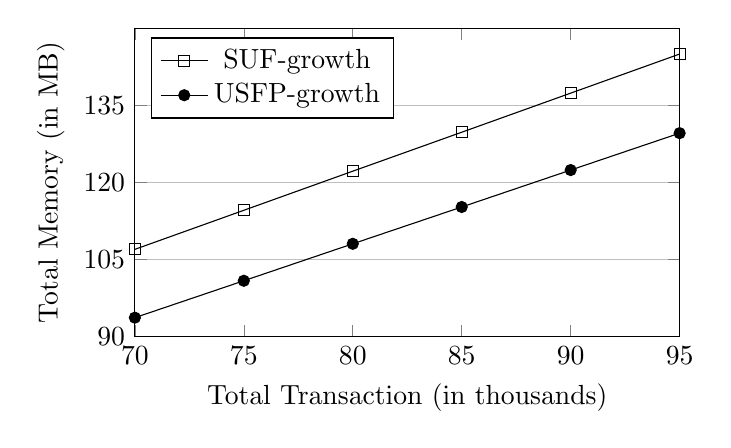
\begin{tikzpicture}
\begin{axis}[
    width=8.5cm,
    height=5.5cm,
    xlabel={Total Transaction (in thousands) },
    ylabel={Total Memory (in MB) },
    xmin=70, xmax=95,
    ymin=90, ymax=150,
    xtick={70,75,80,85,90,95},
    ytick={90,105,120,135},
    legend pos=north west,
    ymajorgrids=true,
    grid style={line width=.2pt,draw=gray!50},
]
 
\addplot[
    solid, every mark/.append style={solid, fill=gray}, mark=square
    ]
    coordinates {
			(70,106.996)
			(75,114.591)
			(80,122.197)
			(85,129.773)
			(90,137.375)
			(95,144.979)

	};
    \addlegendentry{SUF-growth}
\addplot[
    solid, every mark/.append style={solid, fill=black}, mark=*
    ]
    coordinates {
		(70,93.711  )
		(75,100.889 )
		(80,108.076 )
		(85,115.233 )
		(90,122.415 )
		(95,129.591 )

};
    \addlegendentry{USFP-growth}
 
\end{axis}
\end{tikzpicture}
%\end{document}
            \caption{Total Memory vs Total Transaction (in thousand) for T40I10D100K ~\cite{dataset} Dataset }
            \label{result:g_t10_memory_node}
            \end{figure}
        
            \begin{figure}[h]
            \centering
                %mark = star, diamond, square, otimes
%\documentclass{article}
%\usepackage{pgfplots}
%\usepackage[justification=centering]{caption}
%\pgfplotsset{compat=newest}
%\begin{document}
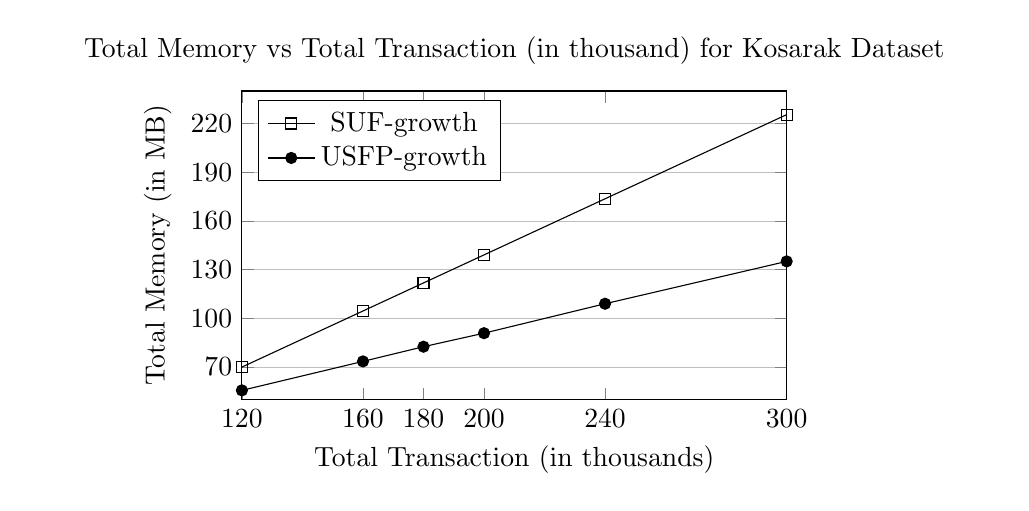
\begin{tikzpicture}
\begin{axis}[
	title={\parbox{\linewidth}{\centering Total Memory vs Total Transaction (in thousand) for Kosarak Dataset}},
    width=8.5cm,
    height=5.5cm,
    xlabel={Total Transaction (in thousands) },
    ylabel={Total Memory (in MB) },
    xmin=120, xmax=300,
    ymin=50	, ymax=240,
    xtick={120,160,180,200,240,300},
    ytick={70,100,130,160,190,220},
    legend pos=north west,
    ymajorgrids=true,
    grid style={line width=.2pt,draw=gray!50},
]
 
\addplot[
    solid, every mark/.append style={solid, fill=gray}, mark=square
    ]
    coordinates {
			(120,	69.945)
			(160,	104.492)
			(180,	121.766)
			(200,	139.039)
			(240,	173.587)
			(300,	225.408)

	};
    \addlegendentry{SUF-growth}
\addplot[
    solid, every mark/.append style={solid, fill=black}, mark=*
    ]
    coordinates {
			(120,	55.607)
			(160,	73.456)
			(180,	82.507)
			(200,	90.835)
			(240,	108.960)
			(300,	135.042)

};
    \addlegendentry{USFP-growth}
 
\end{axis}
\end{tikzpicture}
%\end{document}
            \caption{Total Memory vs Total Transaction (in thousand) for Kosarak ~\cite{dataset} Dataset }
            \label{result:g_k_memory_node}
            \end{figure}

In summary, our proposed \emph{US-tree}, construction \emph{USFP-growth} mining approach is correct, efficient, the scalable, works fine in any configuration (minimum support, window size, batch size). For dense dataset (both real and synthetic) our approach is very efficient. For sparse dataset, this also gives us gain both in memory and running time. The \emph{U\textsuperscript{cap}} value gives much more benefit to share nodes in the \emph{US-tree}. The compactness of \emph{US-tree} is noticeable. Mining compact \emph{US-tree} gives the main surprise in the running time. The \emph{USFP-growth} mining algorithm works nicely without generating no false negatives and a little amount of false positives that can efficiently be removed using the false positive reduction technique.

\section{Conclusion}
In this paper, we have proposed new sliding window based probabilistic strategy for finding frequent patterns from uncertain dynamic data. We have proposed \emph{U\textsuperscript{cap}}, which is the upper bound of existential probability. We have proposed new \emph{US-tree} data-structure that is very compact. For mining, we have introduced \emph{USFP-growth} algorithm that will efficiently and recursively mine frequent patterns from \emph{US-tree}.
For calculating \emph{U\textsuperscript{cap}} value, we have taken upper-bound of existential probability that makes the node sharing possible between same items. For uncertainty property of data, node sharing was very much irregular in existing approaches. In our strategy, node sharing is possible more frequently and this makes the tree more compact and efficient. Our proposed \emph{US-tree} is very compact for possible node sharing much more than existing tree structures (e.g. \emph{SUF-growth} ~\cite{suf_growth}). To handle the stream of data we have proposed to divide the whole transactions into batches and windows that is completely dependent on the system user how much recent data she/he wants to store in the tree. Instead of keeping the support we have kept new meta-information based on \emph{U\textsuperscript{cap}} value that helps further mining. We have developed new algorithm \emph{USFP-growth} mining algorithm that efficiently remove unnecessary patterns from the tree earlier, which helps to improve runtime time efficiency. Conditional candidate tree needed to be mined in our approach, will be less than other approaches. This makes the mining algorithm faster. We have also introduced an efficient strategy to remove the false positives generated by our algorithm. Our comprehensive result study shows that total time (tree construction, tree mining, and false positive reduction) is less than existing approaches (e.g. \emph{SUF-growth} ~\cite{suf_growth}). We also developed a frequent pattern tree which may later be used to mine closed patterns and maximal patterns.
As the frequent pattern mining over the domain of uncertain stream data is a very new, there are some scopes to extend and use our proposed approach as a tool for further research.
\textbf{Firstly,} we have introduced probabilistic model for calculating \emph{U\textsuperscript{cap}} value. This value can be studied and updated to find both upper and lower bound of existential probability.
\textbf{Secondly,} as data-set we have worked on is the stream data, which is dynamic, can be changed dynamically with time. Once an item comes to the top of the \emph{US-tree} stays there at least it becomes oldest data although may be very much infrequent in the recent data. This case may make the tree not compact that was possible. As data stream cannot be read more than once. So no previously assumption can be done to the tree. So some re-construction after new batch inserted into the window will possibly be the one of the major optimization of the tree.


\bibliographystyle{IEEEtran}
%\bibliography{mybib}
\bibliography{Bibliography}

% that's all folks
\end{document}


